\documentclass{beamer}
%
% Choose how your presentation looks.
%
% For more themes, color themes and font themes, see:
% http://deic.uab.es/~iblanes/beamer_gallery/index_by_theme.html
%
\mode<presentation>
{
  \usetheme{default}      % or try Darmstadt, Madrid, Warsaw, ...
  \usecolortheme{default} % or try albatross, beaver, crane, ...
  \usefonttheme{default}  % or try serif, structurebold, ...
  \setbeamertemplate{navigation symbols}{}
  \setbeamertemplate{caption}[numbered]
} 
\usepackage{amsthm}
\usepackage{polski}
\usepackage[utf8x]{inputenc}
\usepackage{enumitem}
\usepackage{epstopdf}
\title[Your Short Title]{Your Presentation}
\author{Andrzej Kokosza}
\date{Oblicze 2016}


\makeatletter
\newenvironment<>{proofs}[1][\proofname]{%
    \par
    \def\insertproofname{#1\@addpunct{.}}%
    \usebeamertemplate{proof begin}#2}
  {\usebeamertemplate{proof end}}
\makeatother


\newtheorem{definicja}{Definicja}
\newtheorem{przyklad}{Przykład}
\newtheorem{twierdzenie}{Twierdzenie}
\newtheorem{lemat}{Lemat}
\newtheorem{wn}{Wniosek}

\begin{document}

\begin{frame}
  \titlepage
\end{frame}

% Uncomment these lines for an automatically generated outline.
%\begin{frame}{Outline}
%  \tableofcontents
%\end{frame}

\section{Aksjomaty}

\begin{frame}{Aksjomaty}

\begin{figure}[!htb]
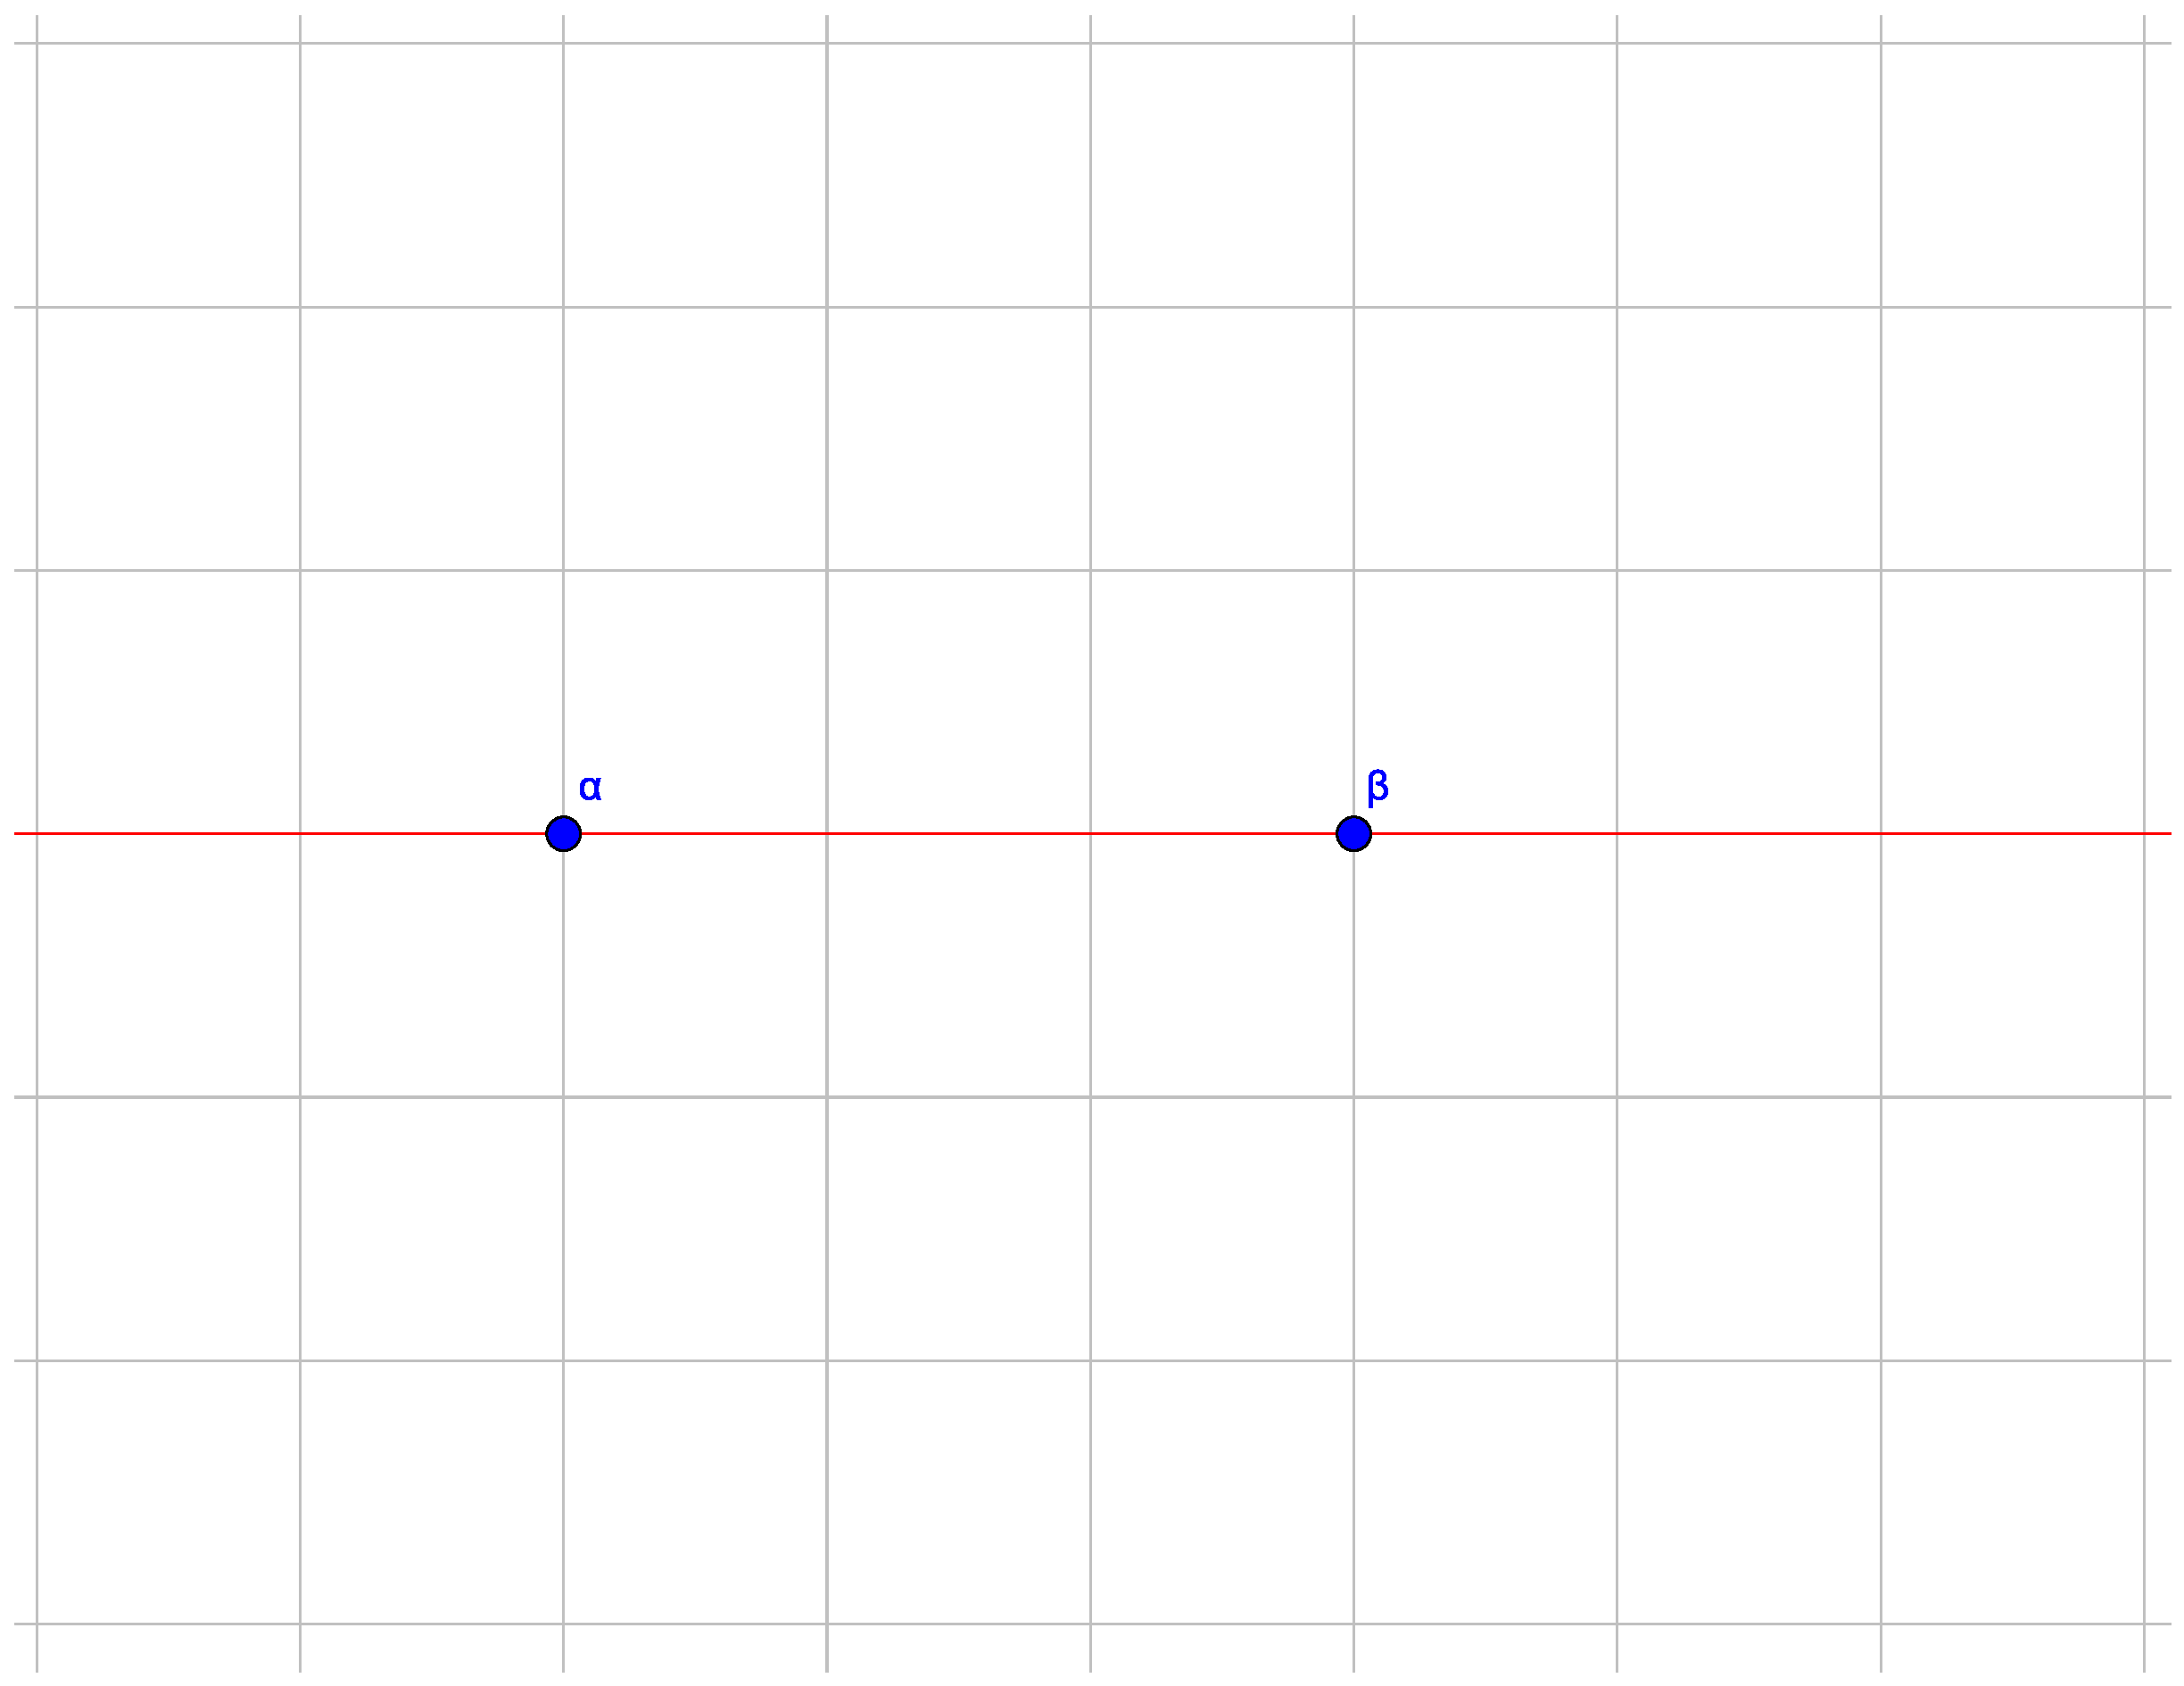
\includegraphics[scale=0.2]{C1.eps}
\label{fig:C1}
\end{figure}

\begin{block}{}
\centering
(C1)  Dwa punkty $\alpha\not=\beta$ można połączyć prostą.
\end{block}

\end{frame}


\begin{frame}{Aksjomaty}

\begin{figure}[!htb]
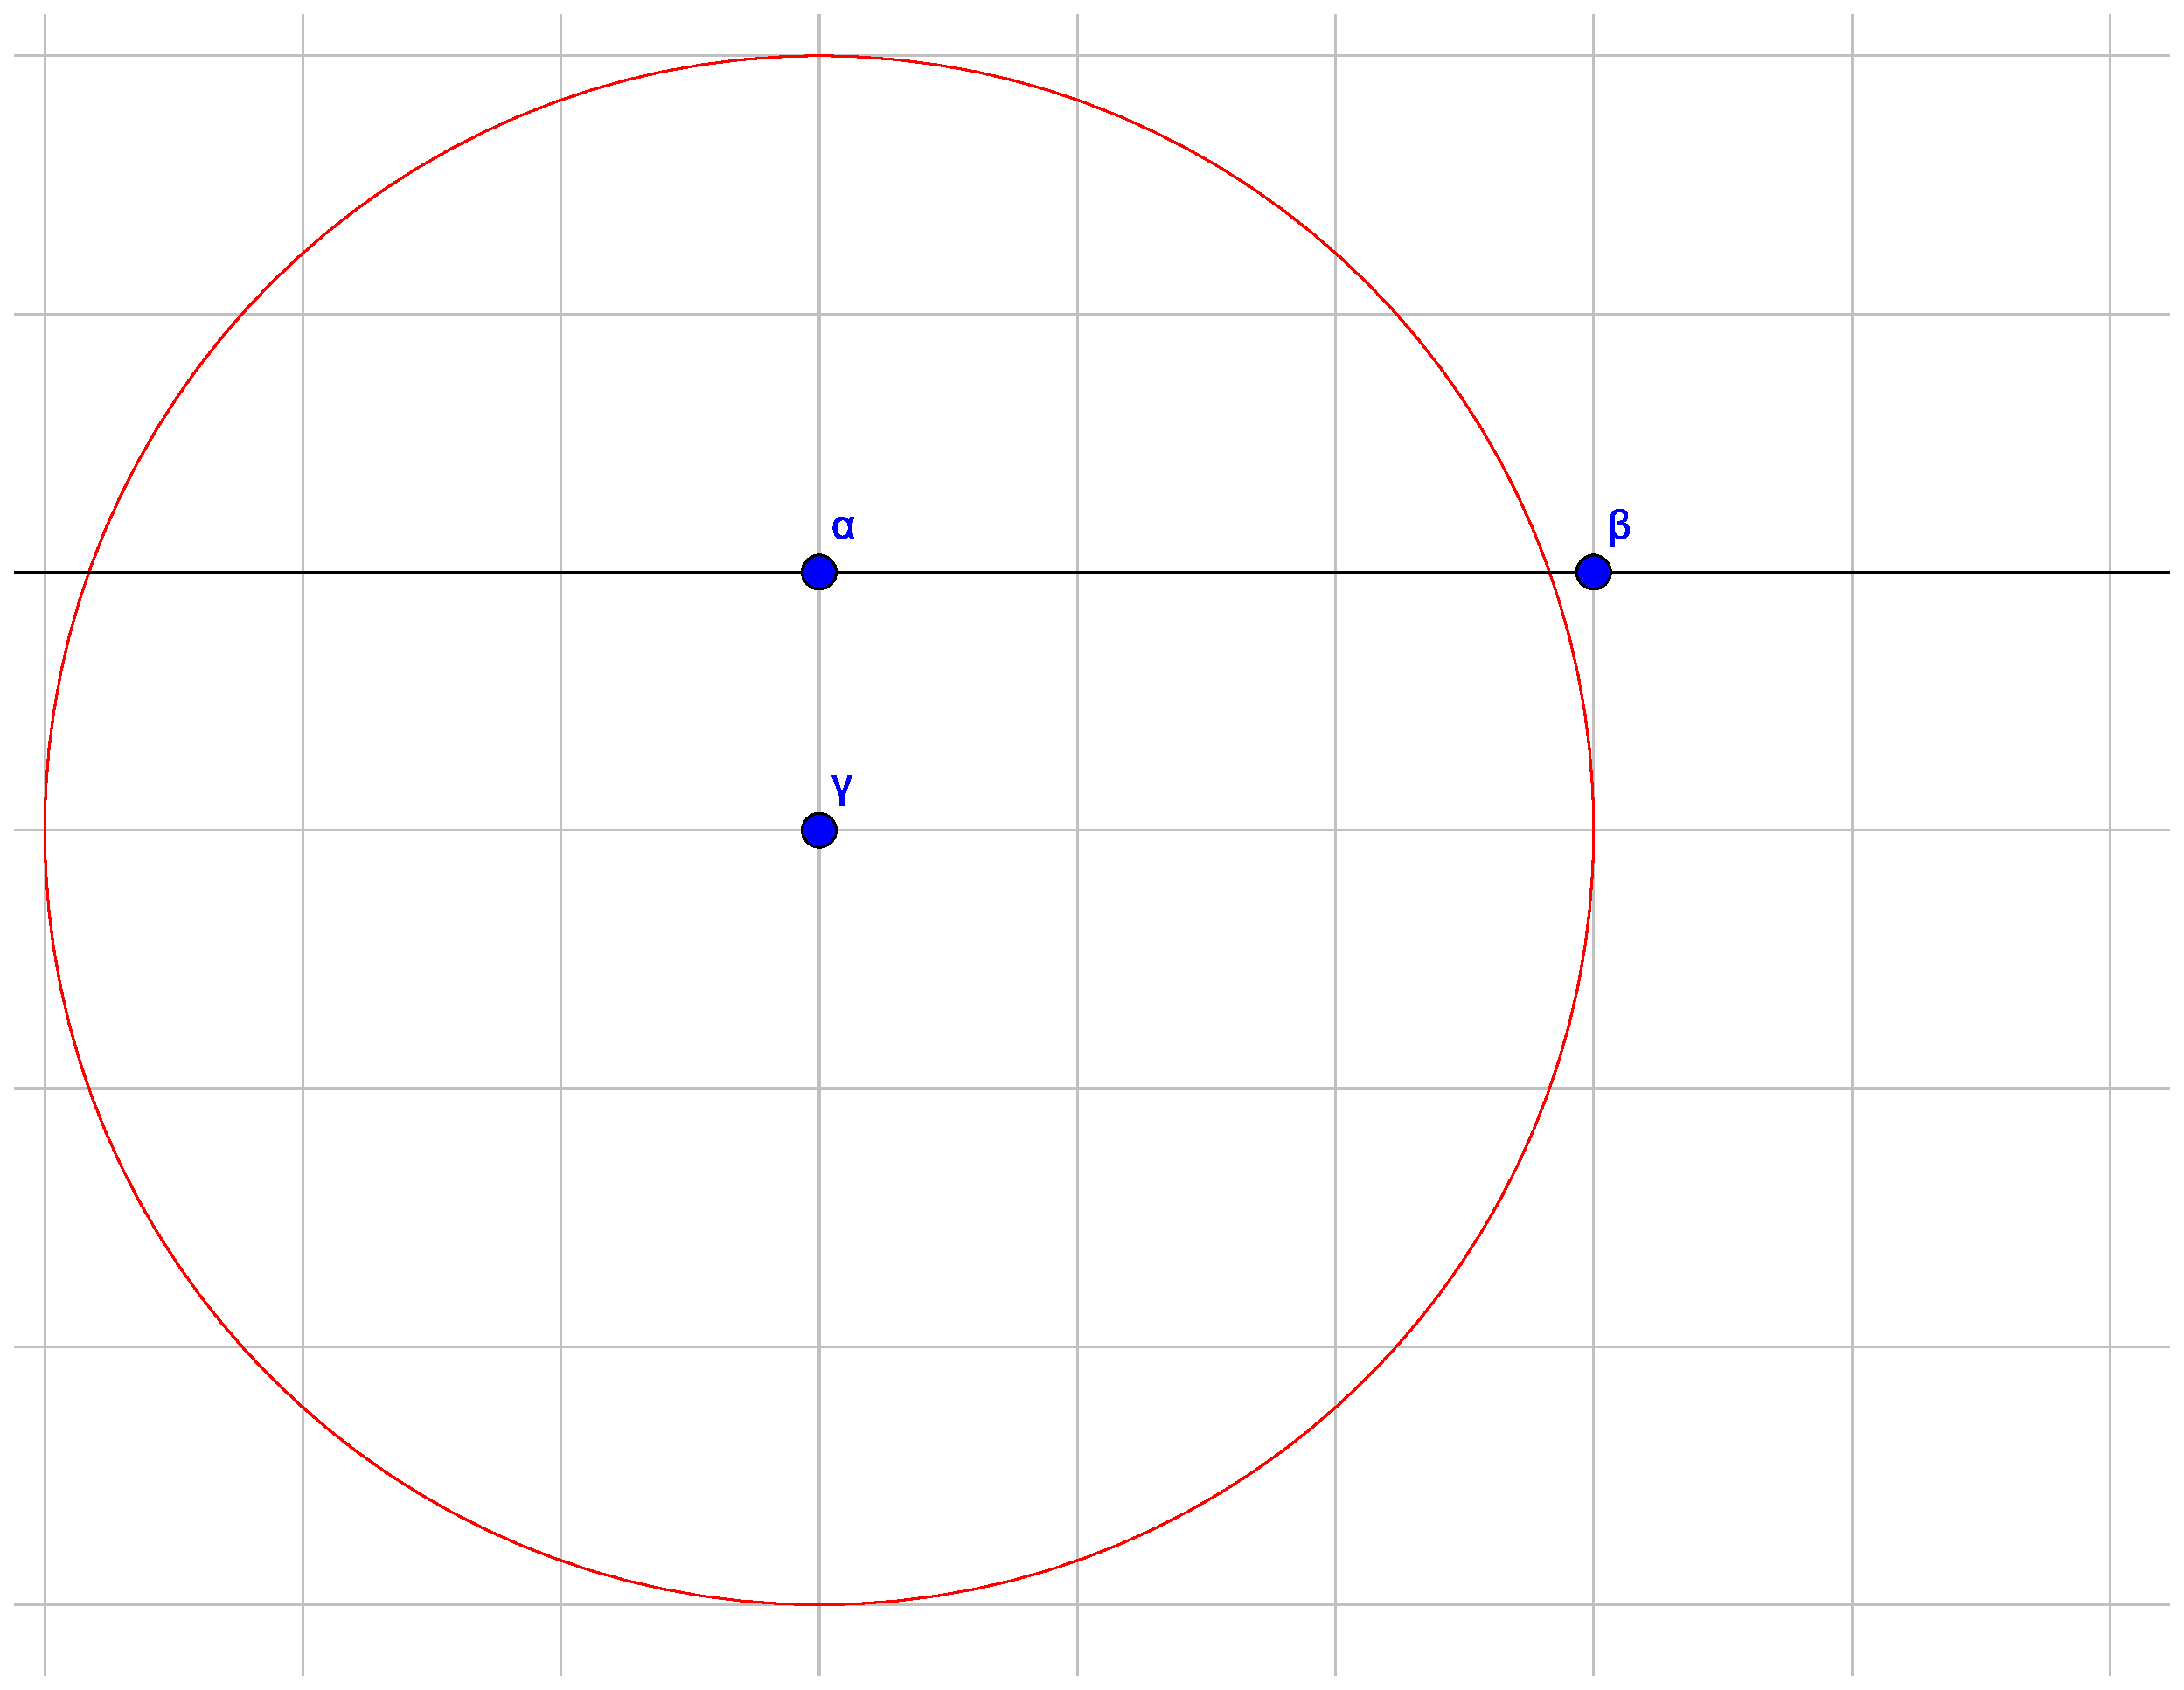
\includegraphics[scale=0.2]{C2.eps}
\label{fig:C2}
\end{figure}

\begin{block}{}
\centering
(C2)  Dla puntów $\alpha\not=\beta$ i $\gamma$ można utworzyć okrąg o środku w $\gamma$ i promieniu 
$|\alpha\beta$
\end{block}

\end{frame}


\begin{frame}{Aksjomaty}

\begin{figure}[!htb]
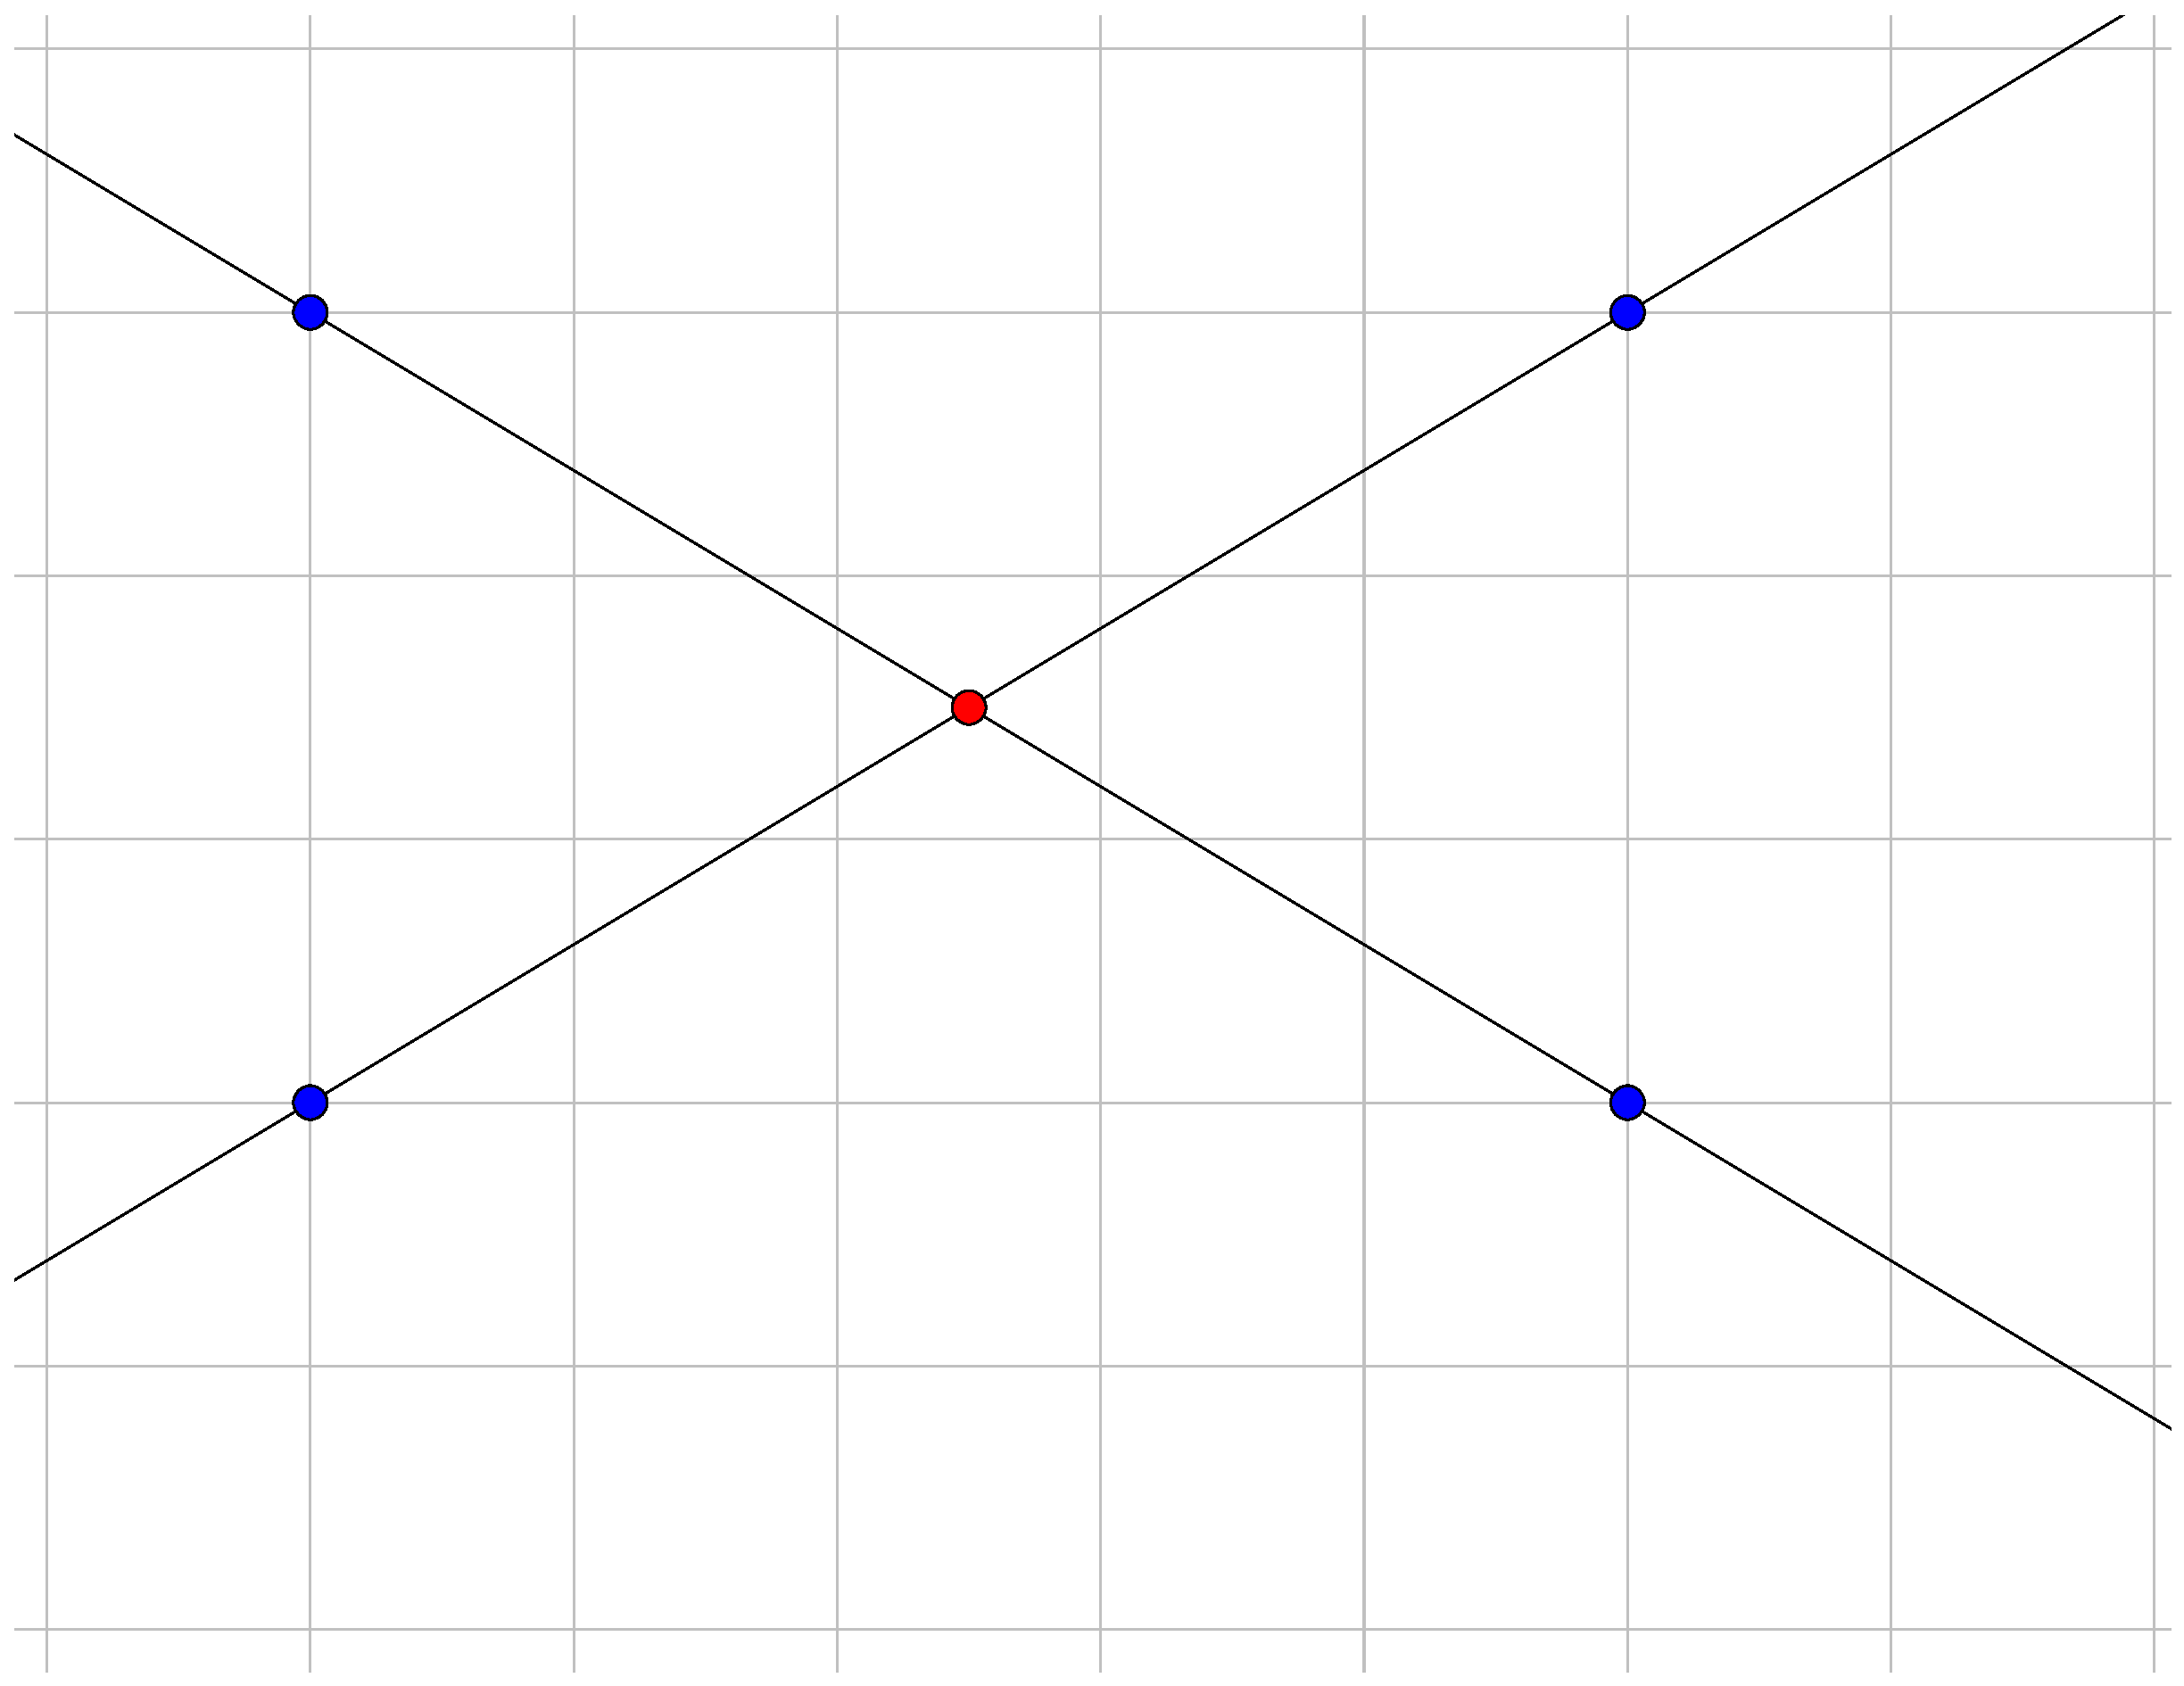
\includegraphics[scale=0.2]{P1.eps}
\label{fig:P1}
\end{figure}

\begin{block}{}
\centering
(P1)  Punkt powstaje poprzez przecięcie 2 prostych. 
\end{block}

\end{frame}


\begin{frame}{Aksjomaty}

\begin{figure}[!htb]
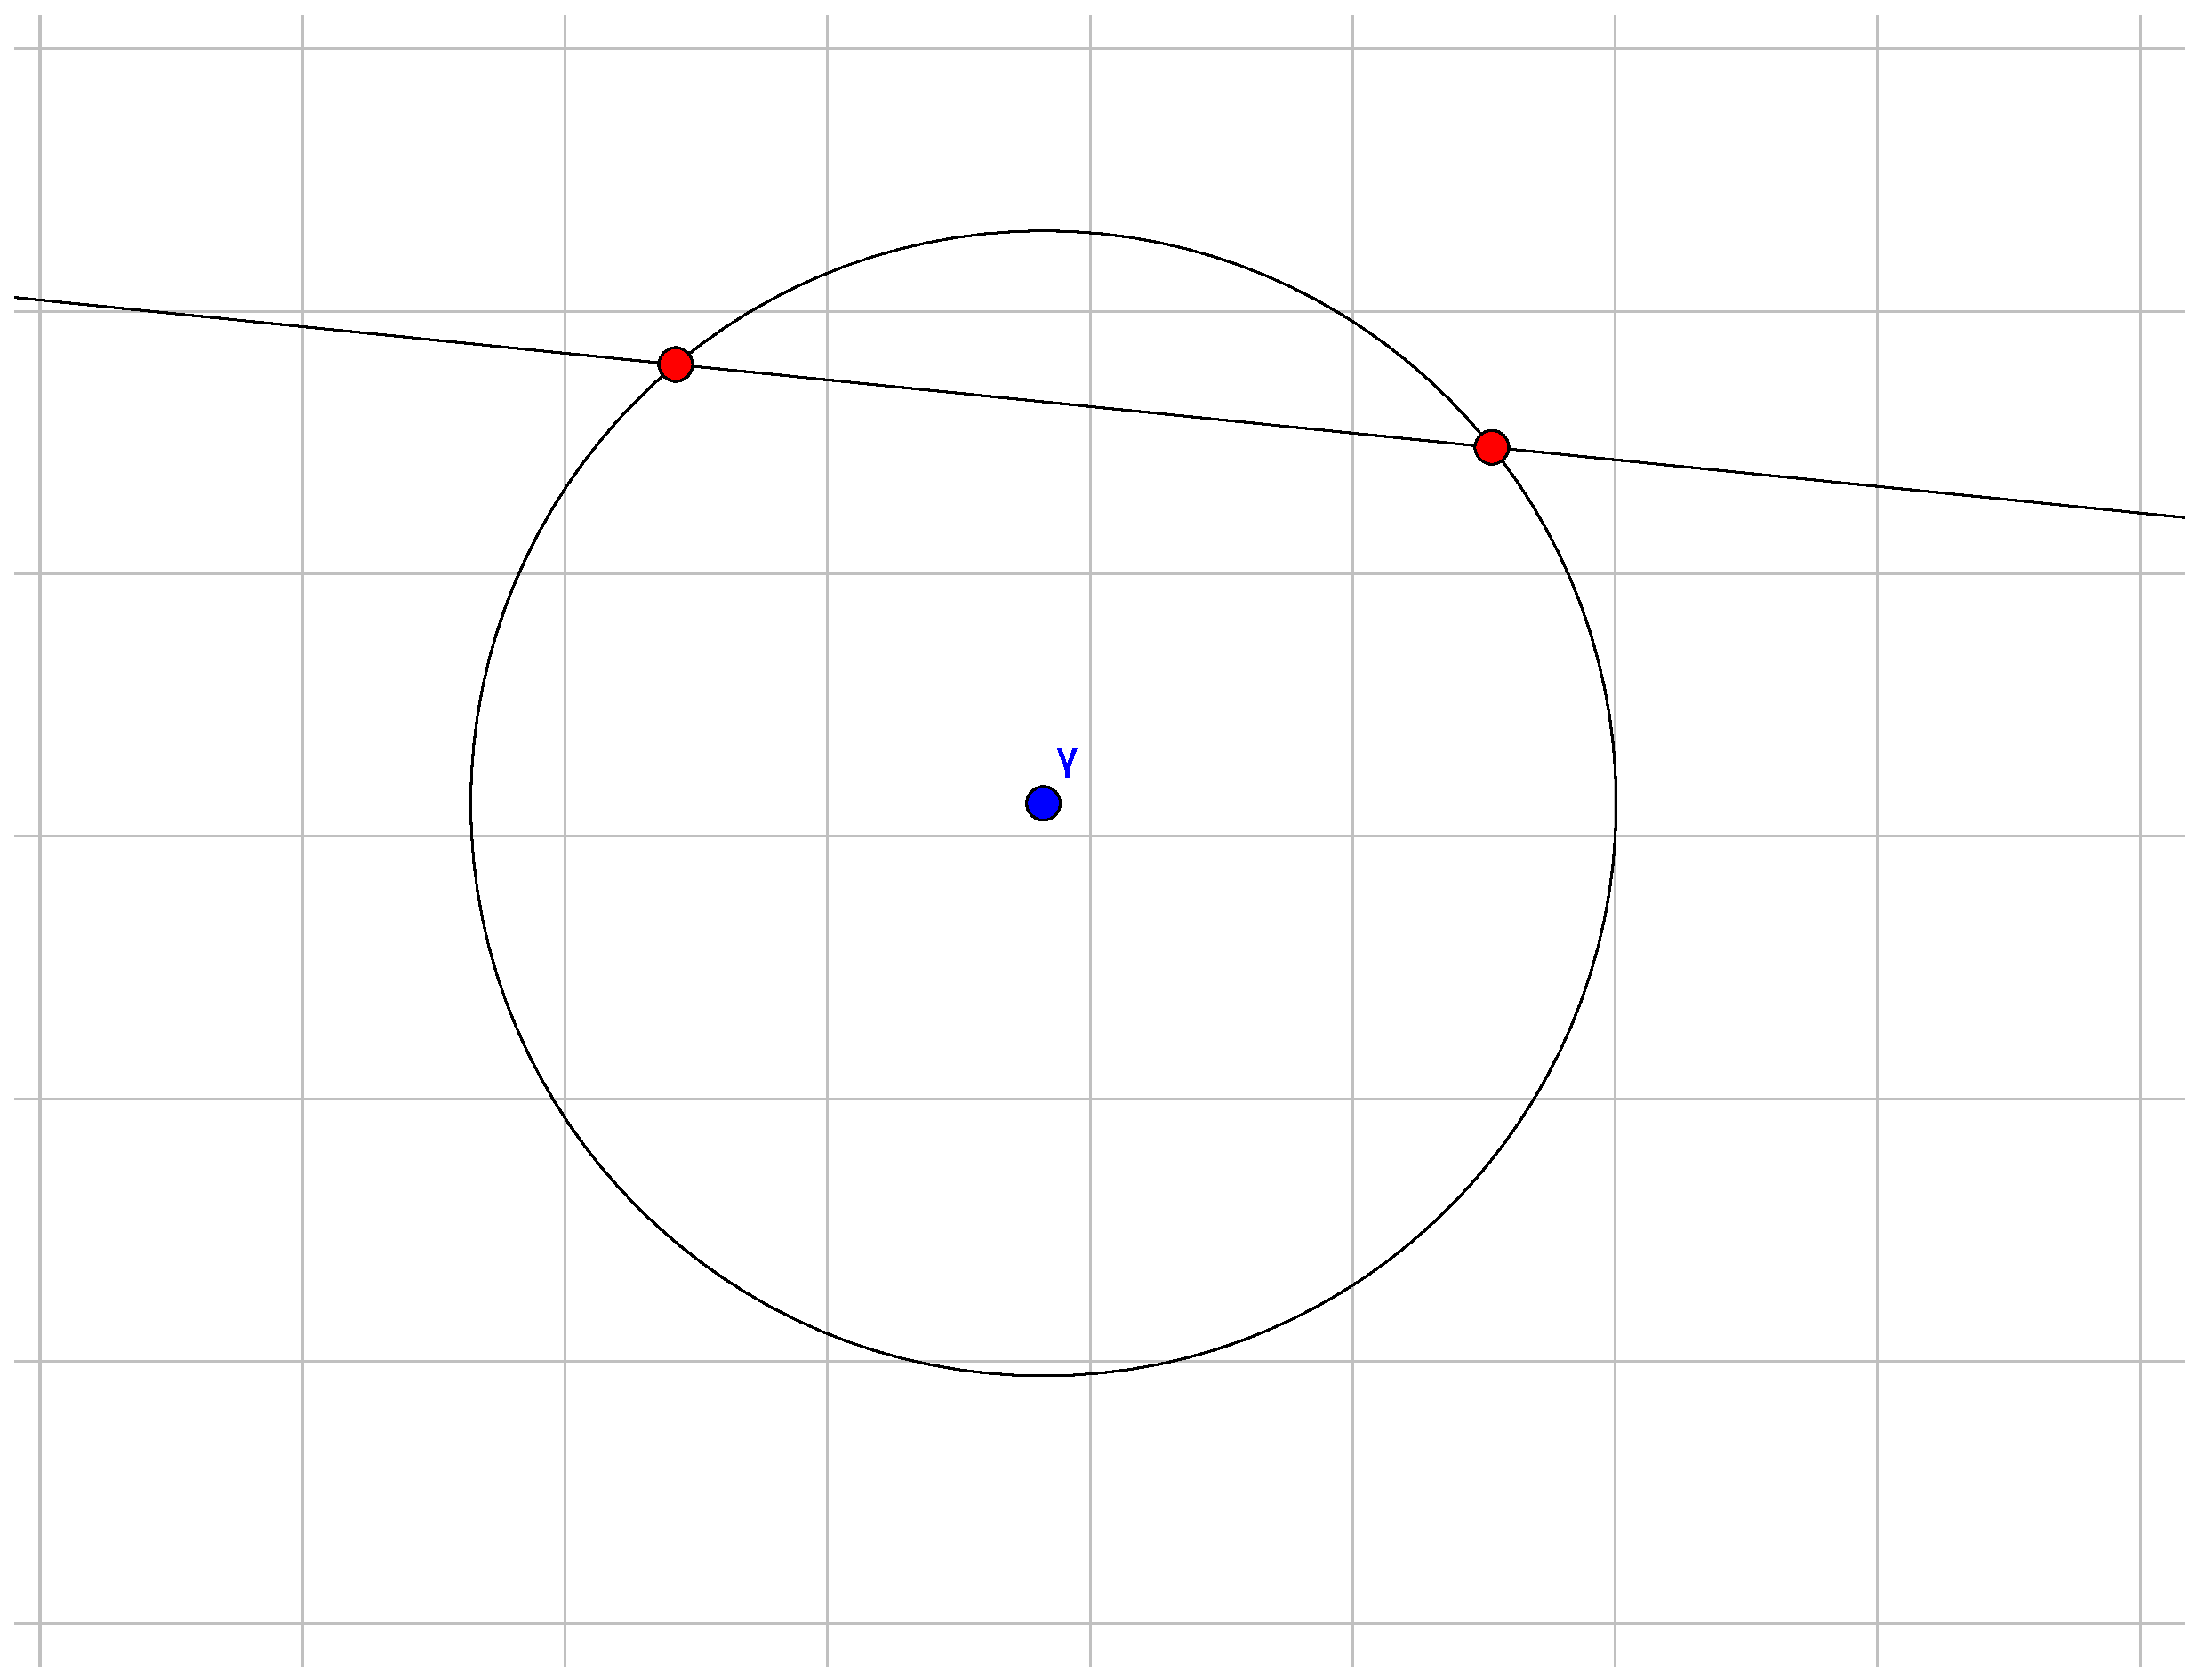
\includegraphics[scale=0.2]{P2.eps}
\label{fig:P2}
\end{figure}

\begin{block}{}
\centering
(P2)  Punkt powstaje przez przecięcie prostej i okręgu.
\end{block}

\end{frame}


\begin{frame}{Aksjomaty}

\begin{figure}[!htb]
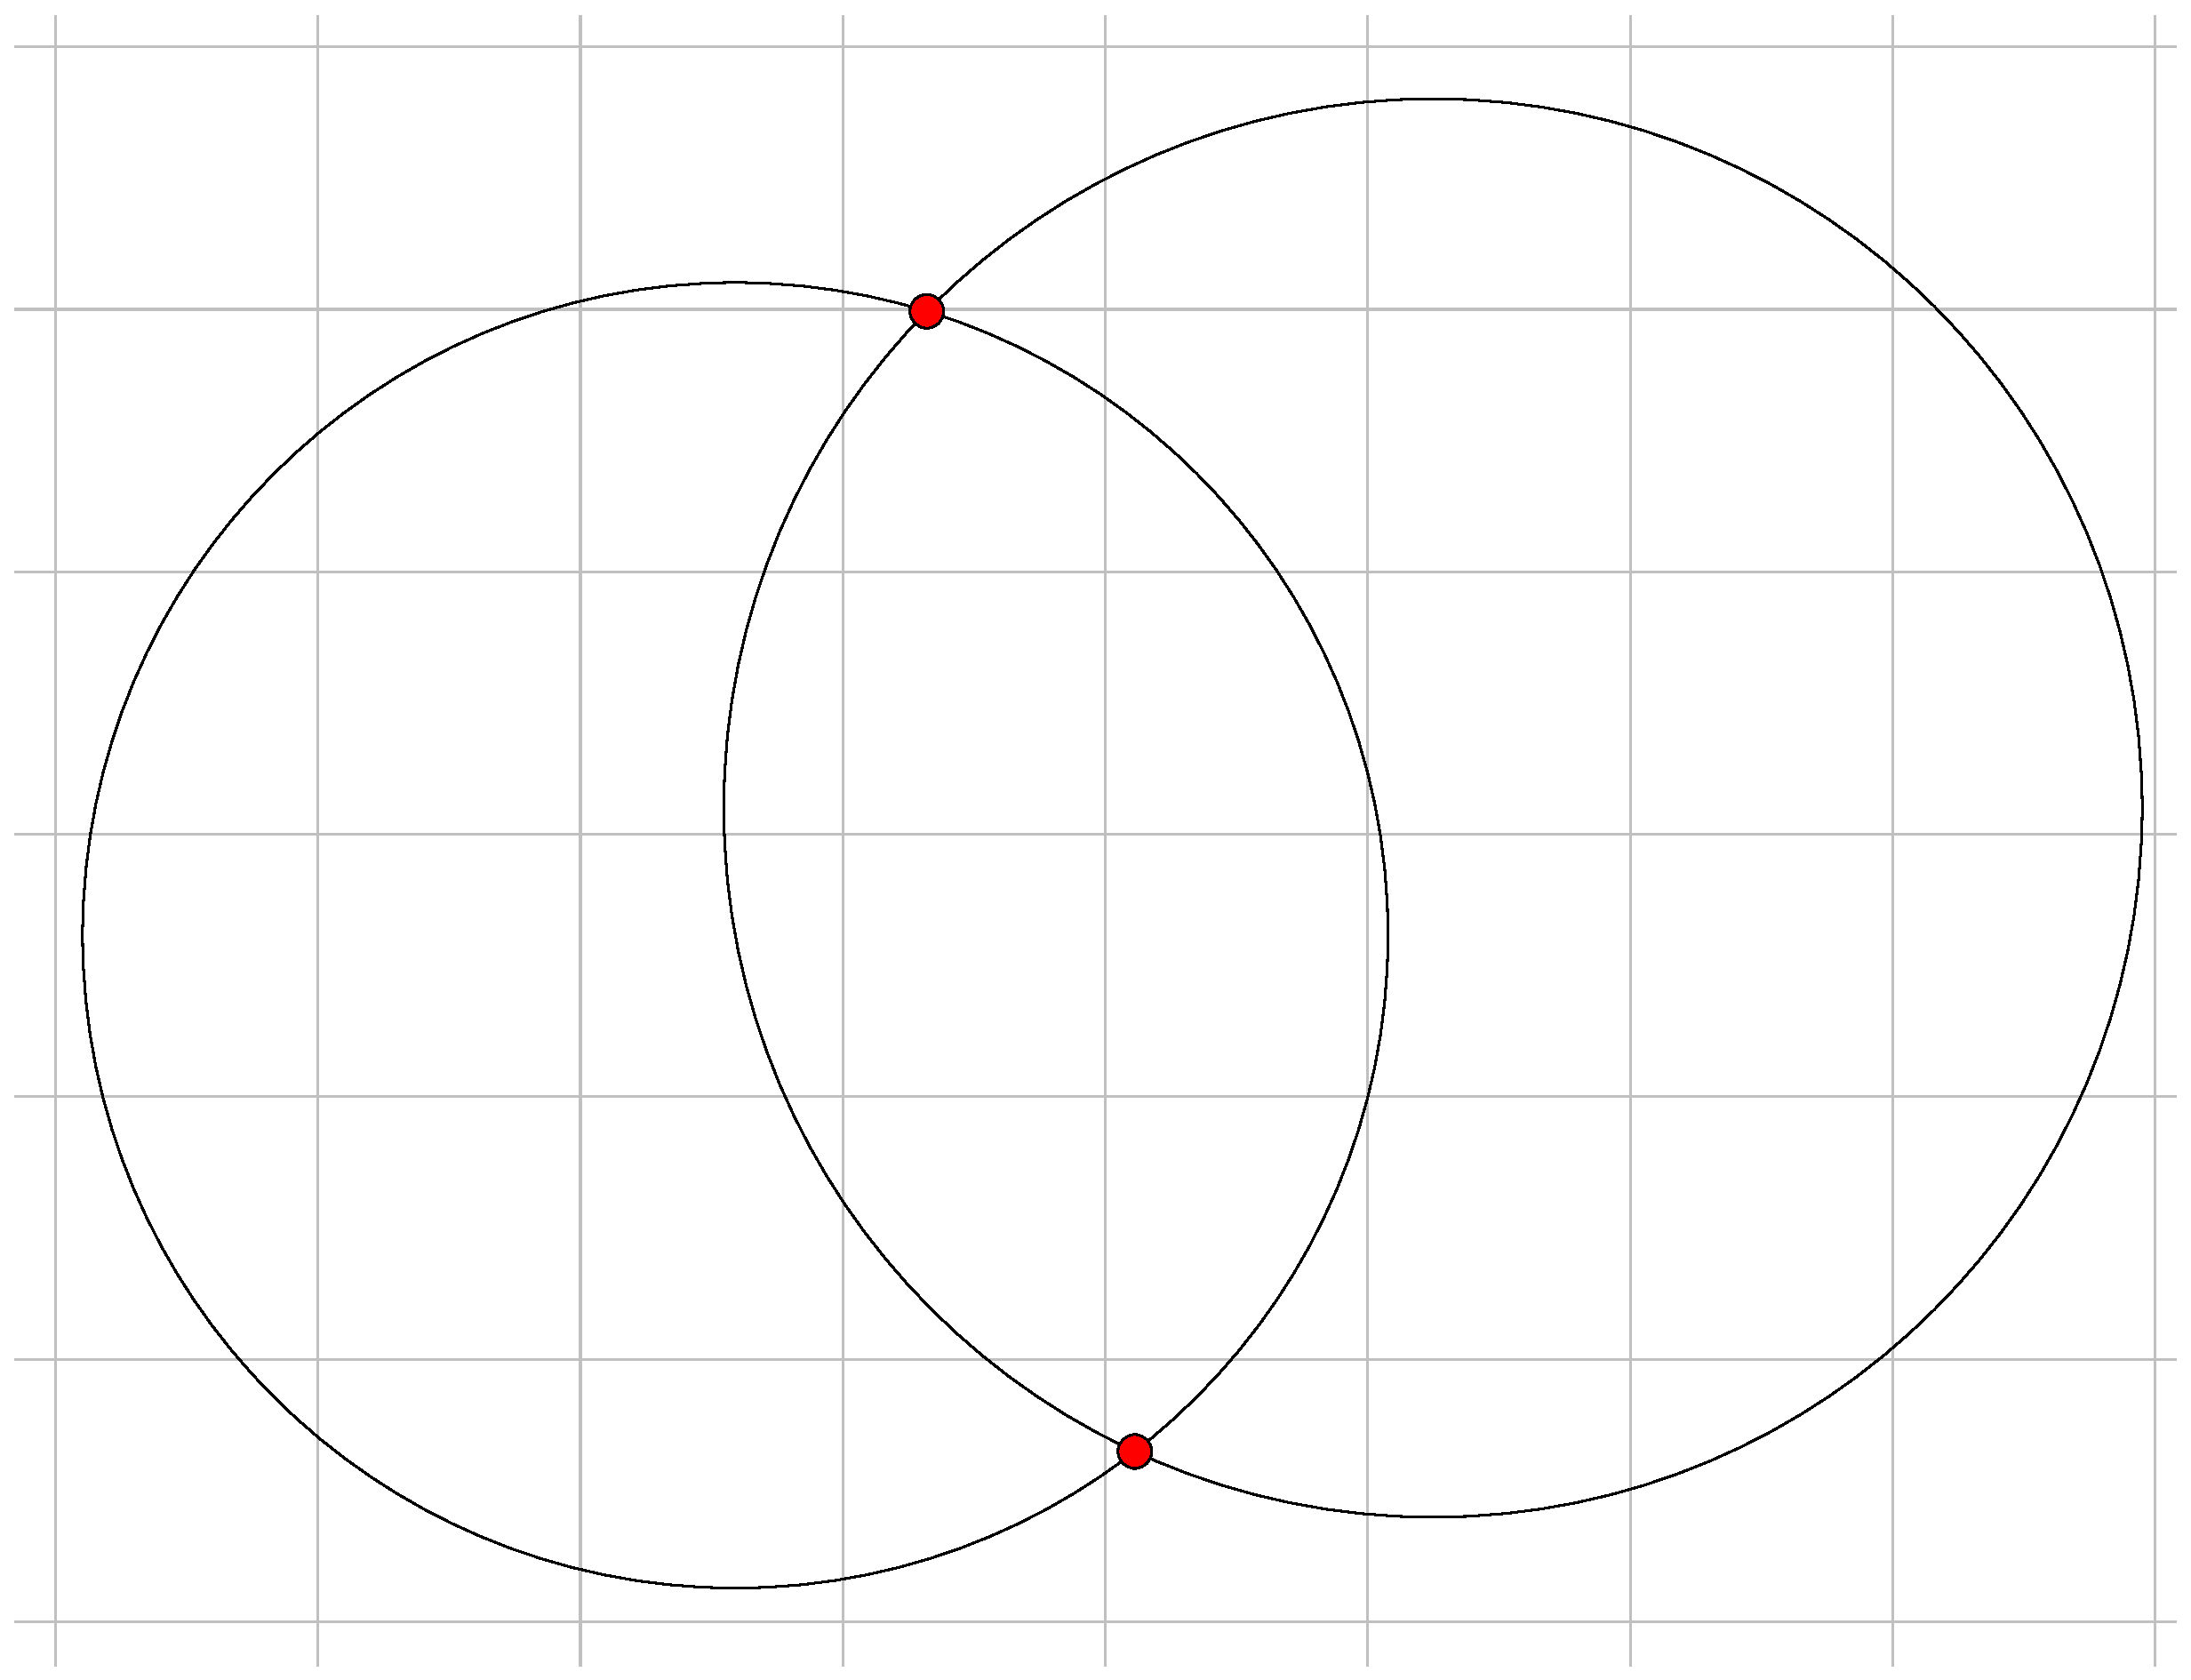
\includegraphics[scale=0.2]{P3.eps}
\label{fig:digraph}
\end{figure}

\begin{block}{}
\centering
(P3)  Punkt powstaje przez przecięcie dwóch okręgów.
\end{block}

\end{frame}

\section{Liczby Konstruowalne}


\begin{frame}{Liczby Konstruowalne}
\begin{definicja}
Liczba zespololona jest konstruowalna, gdy można utworzyć ją za pomocą aksjomatów C1, C2, P1, P2, P3 w skończonej liczbie kroków. z liczb $0$, $1$.
\end{definicja}
\end{frame}

\begin{frame}{Liczby Konstruowalne}
\begin{przyklad}
Liczby naturalne
\begin{figure}[!htb]
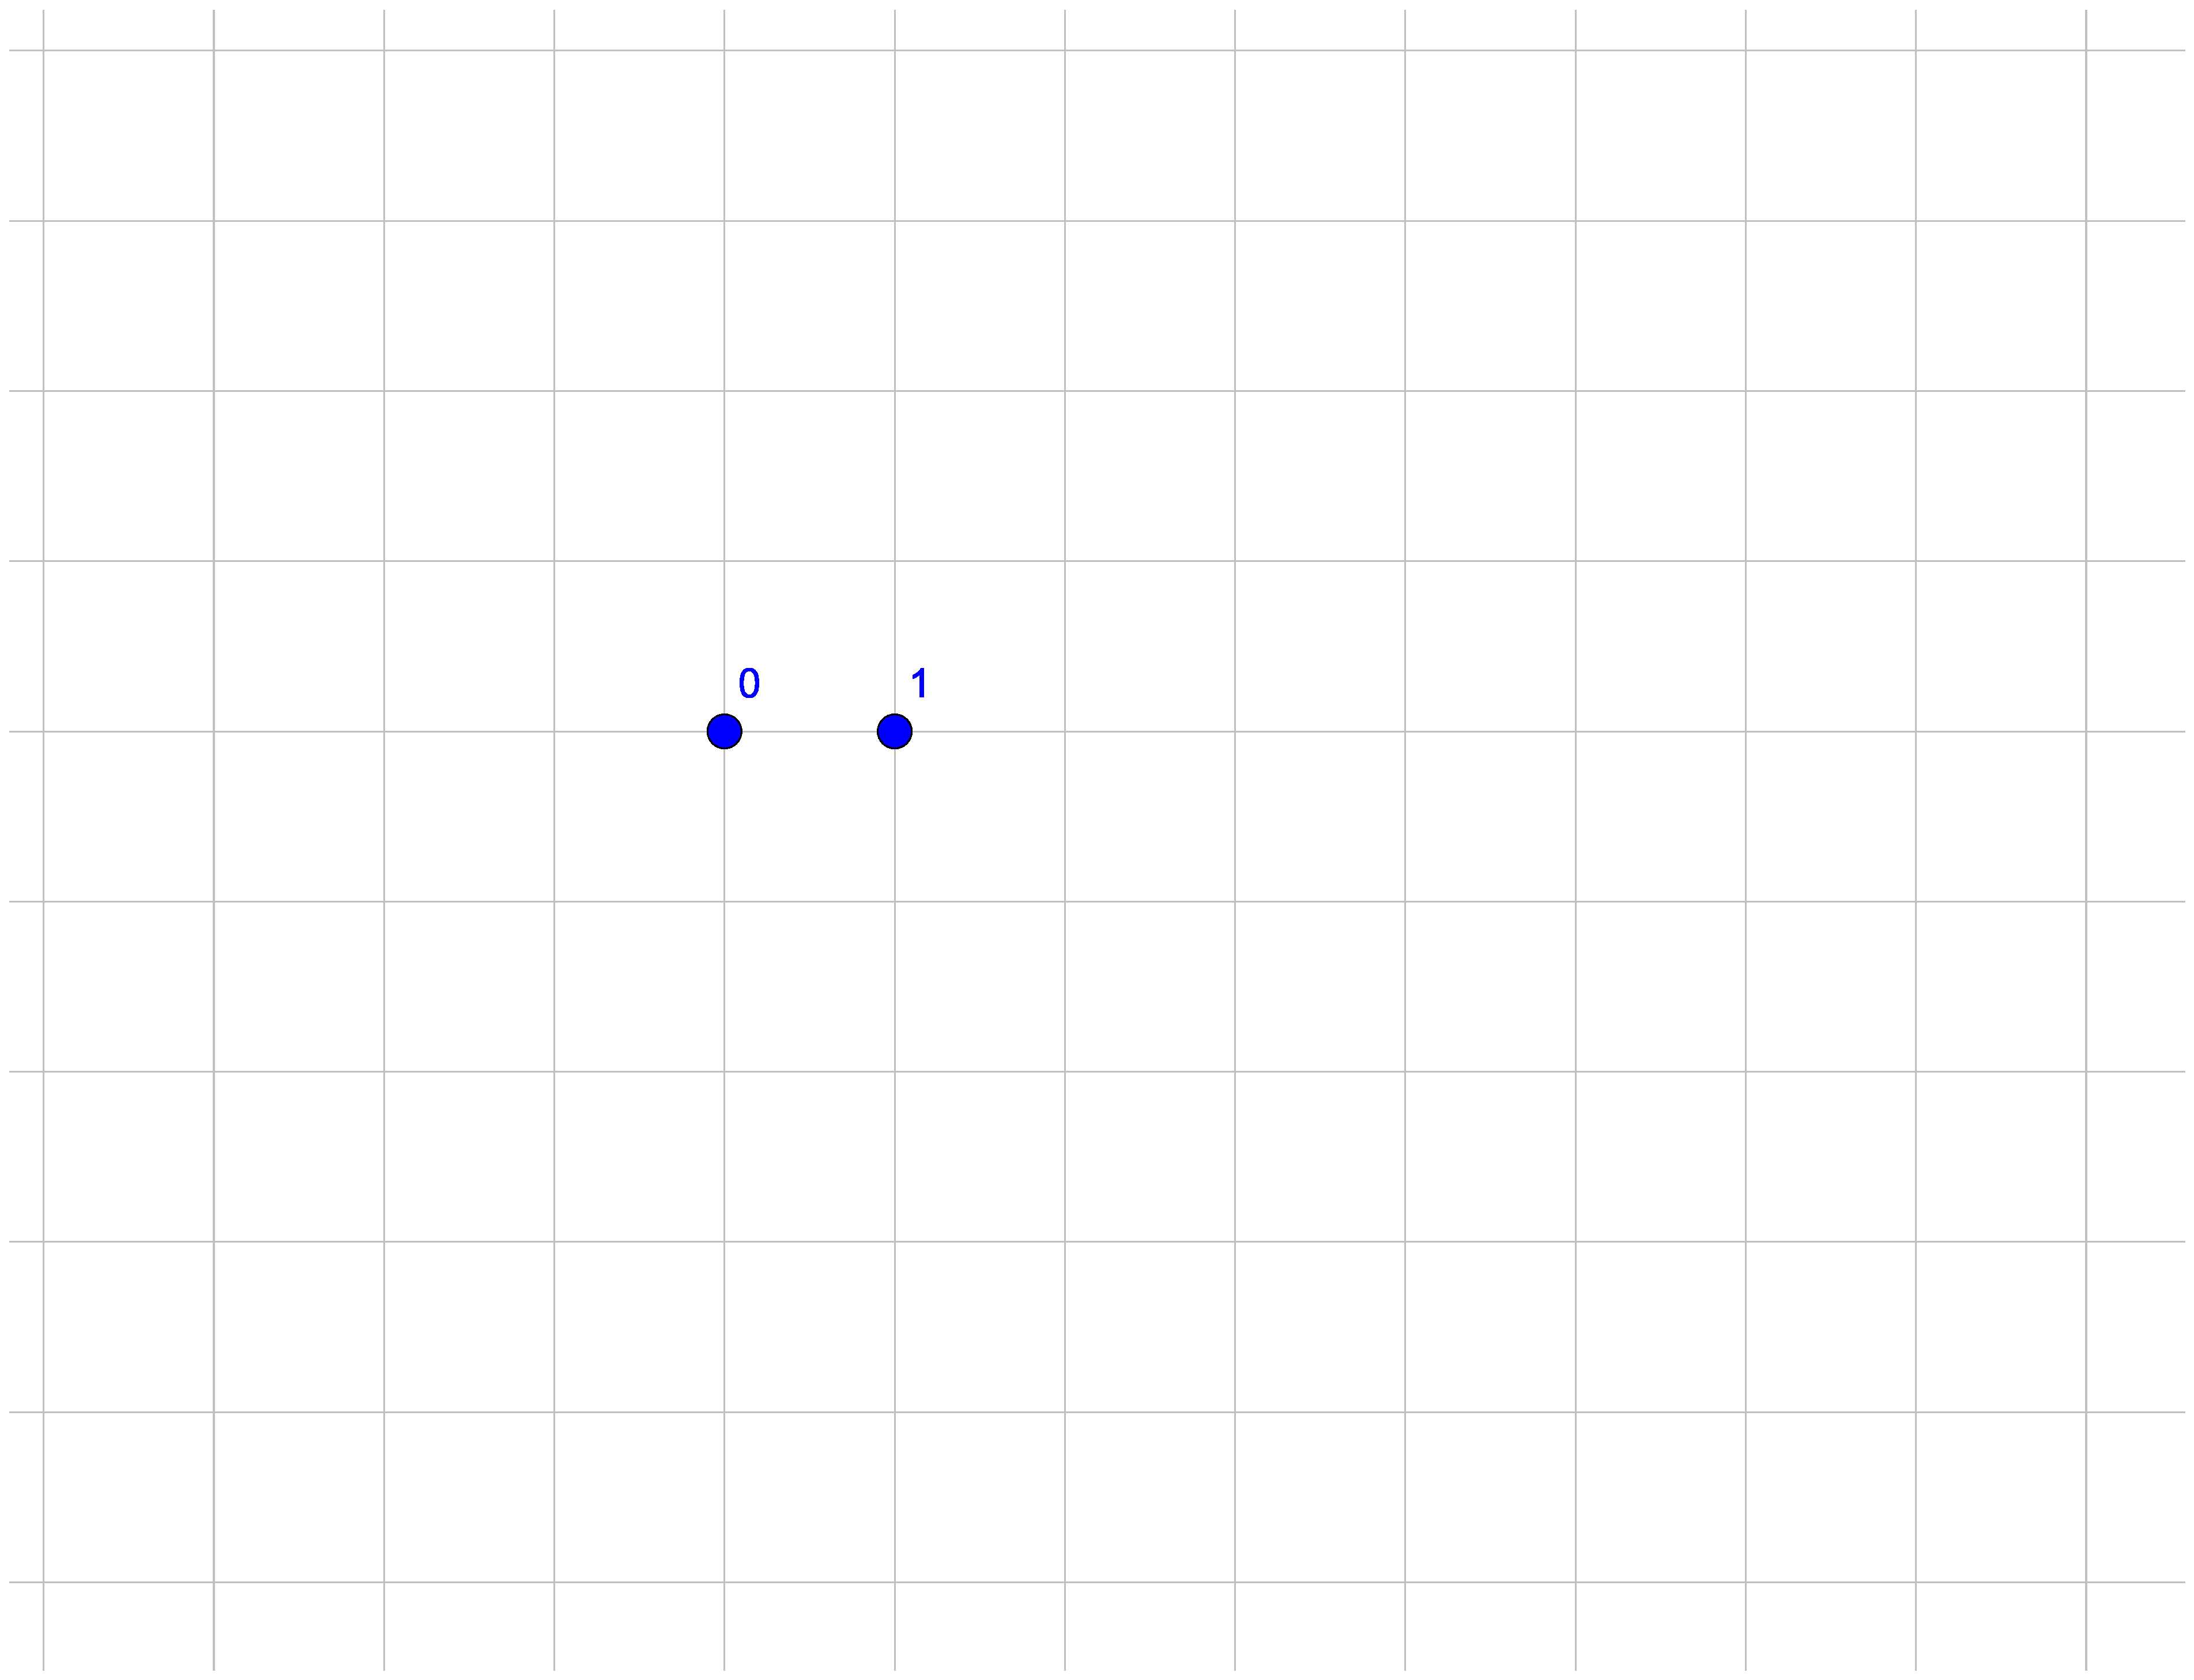
\includegraphics[scale=0.1]{ex1.eps}
\label{fig:ex1}
\end{figure}
\end{przyklad}
\end{frame}

\begin{frame}{Liczby Konstruowalne}
\begin{przyklad}
Liczby naturalne
\begin{figure}[!htb]
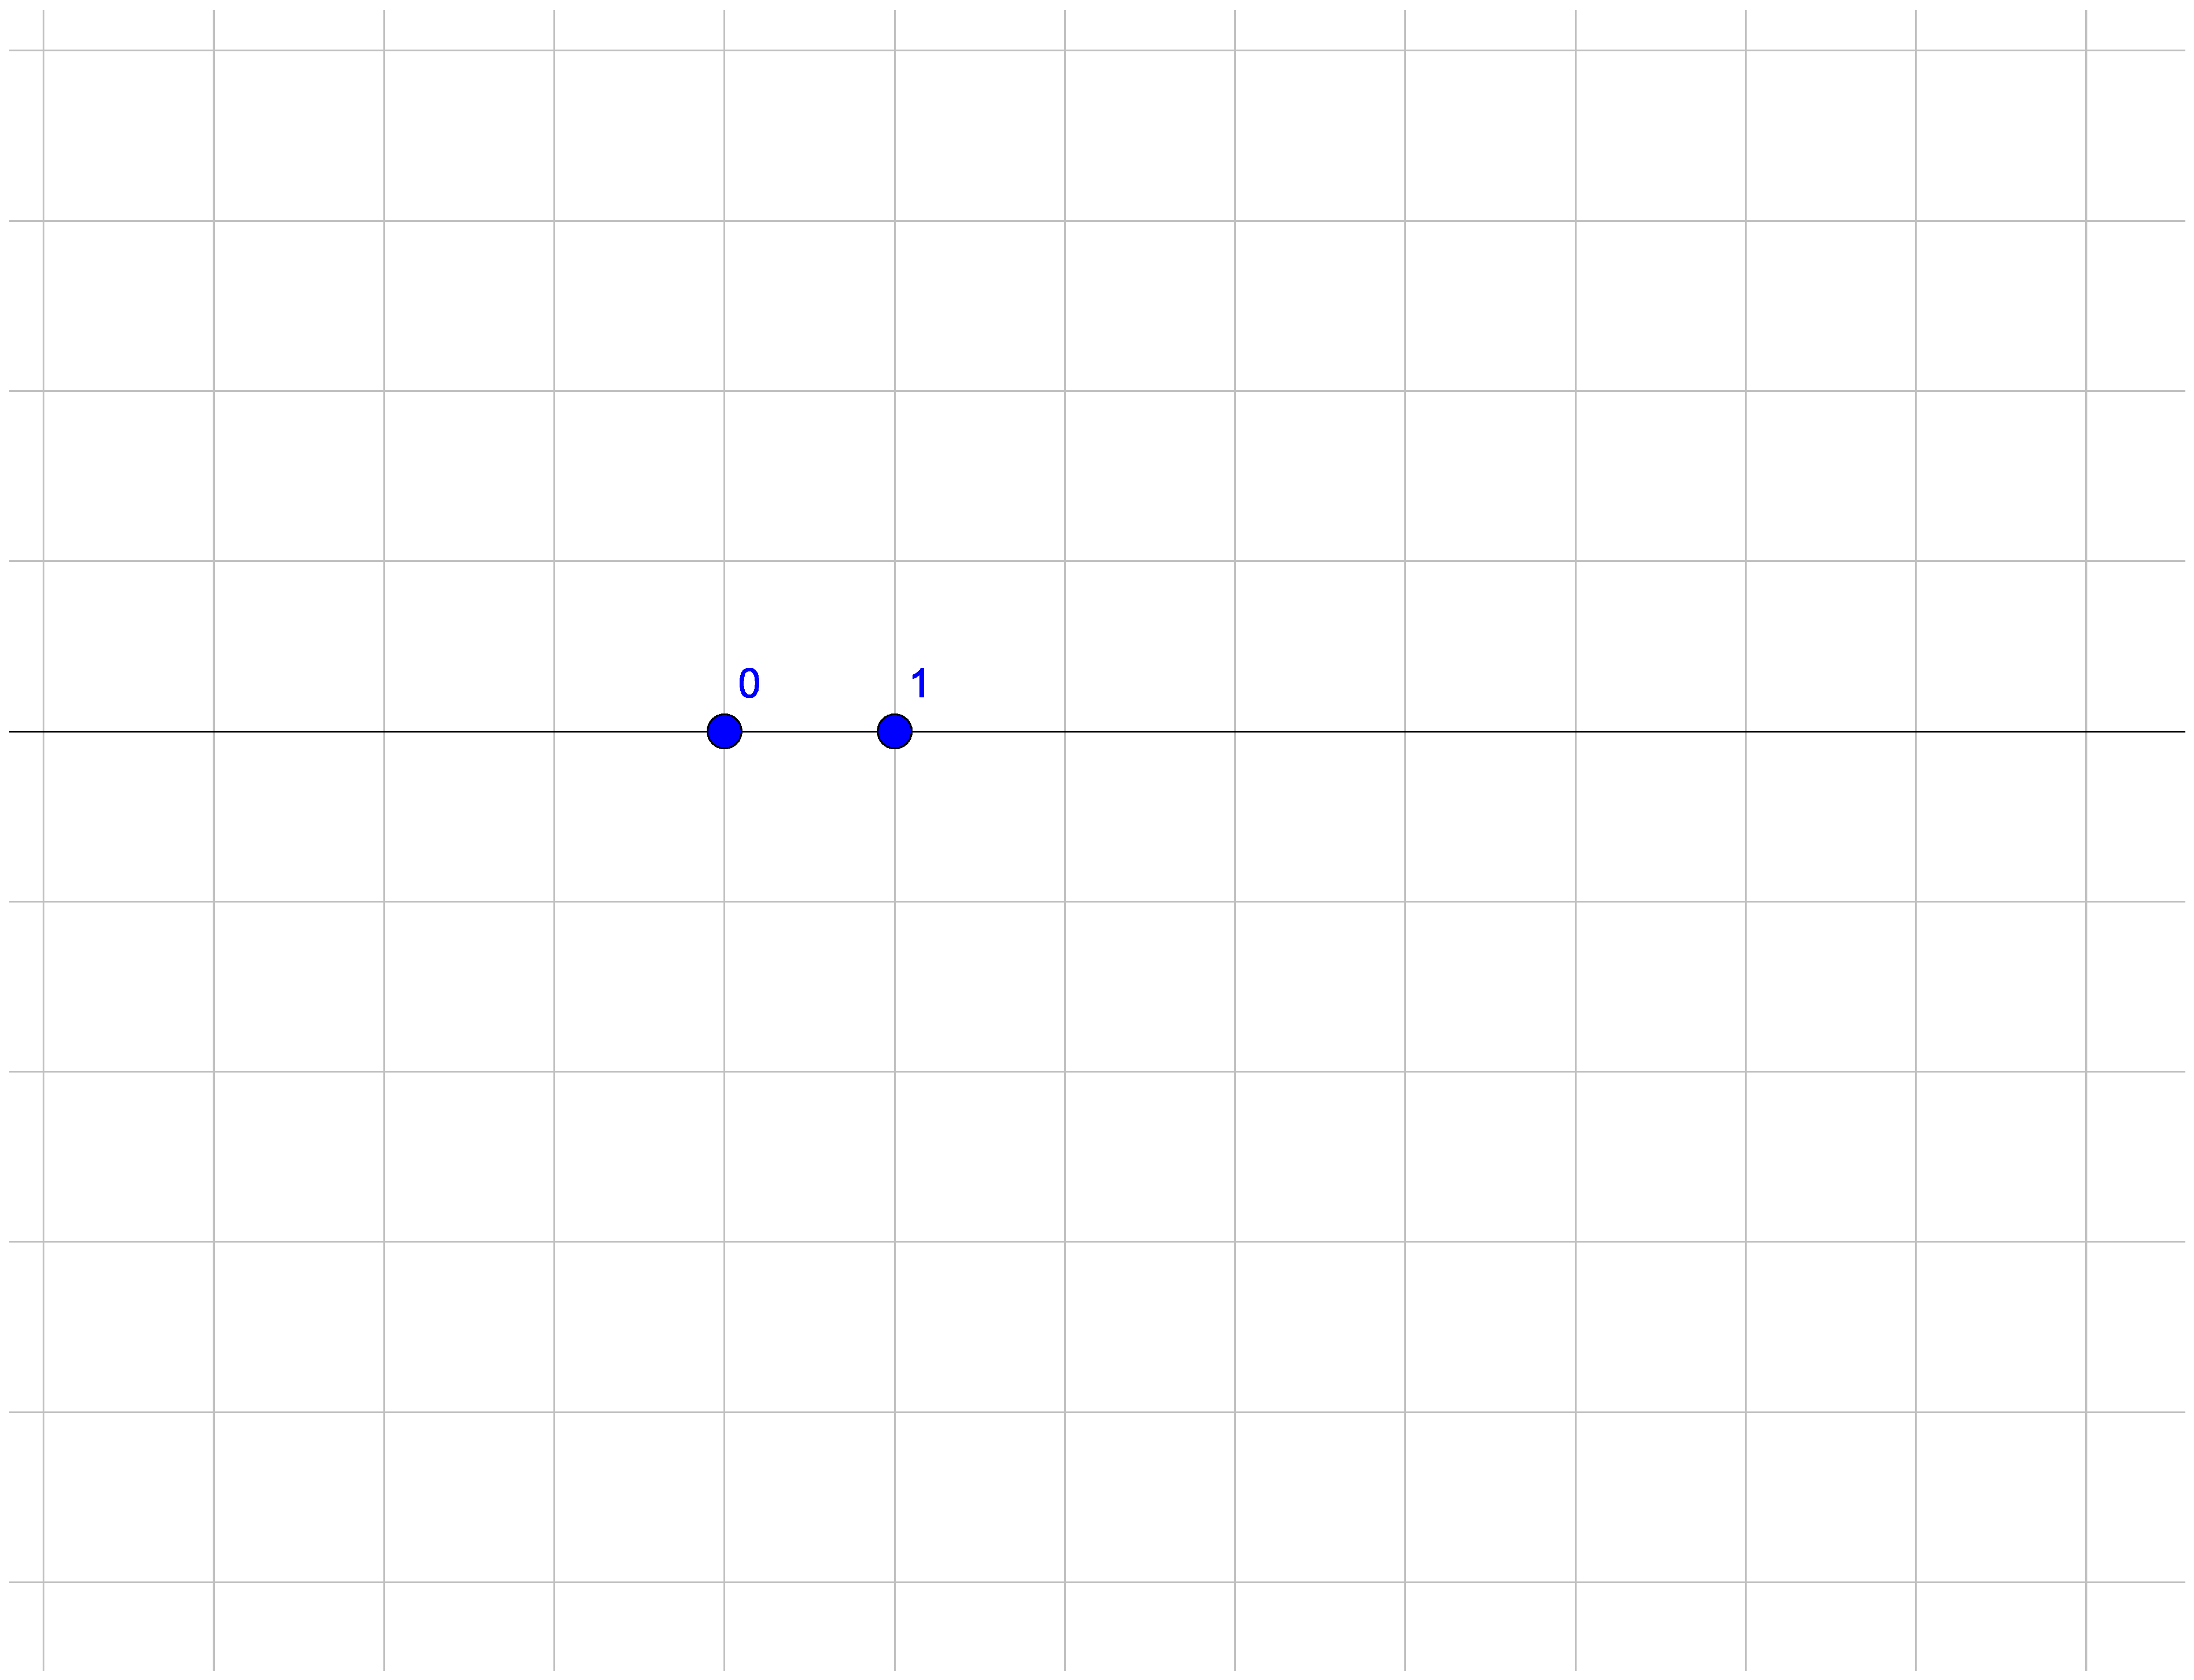
\includegraphics[scale=0.1]{ex2.eps}
\label{fig:ex2}
\end{figure}
\end{przyklad}
\end{frame}

\begin{frame}{Liczby Konstruowalne}
\begin{przyklad}
Liczby naturalne
\begin{figure}[!htb]
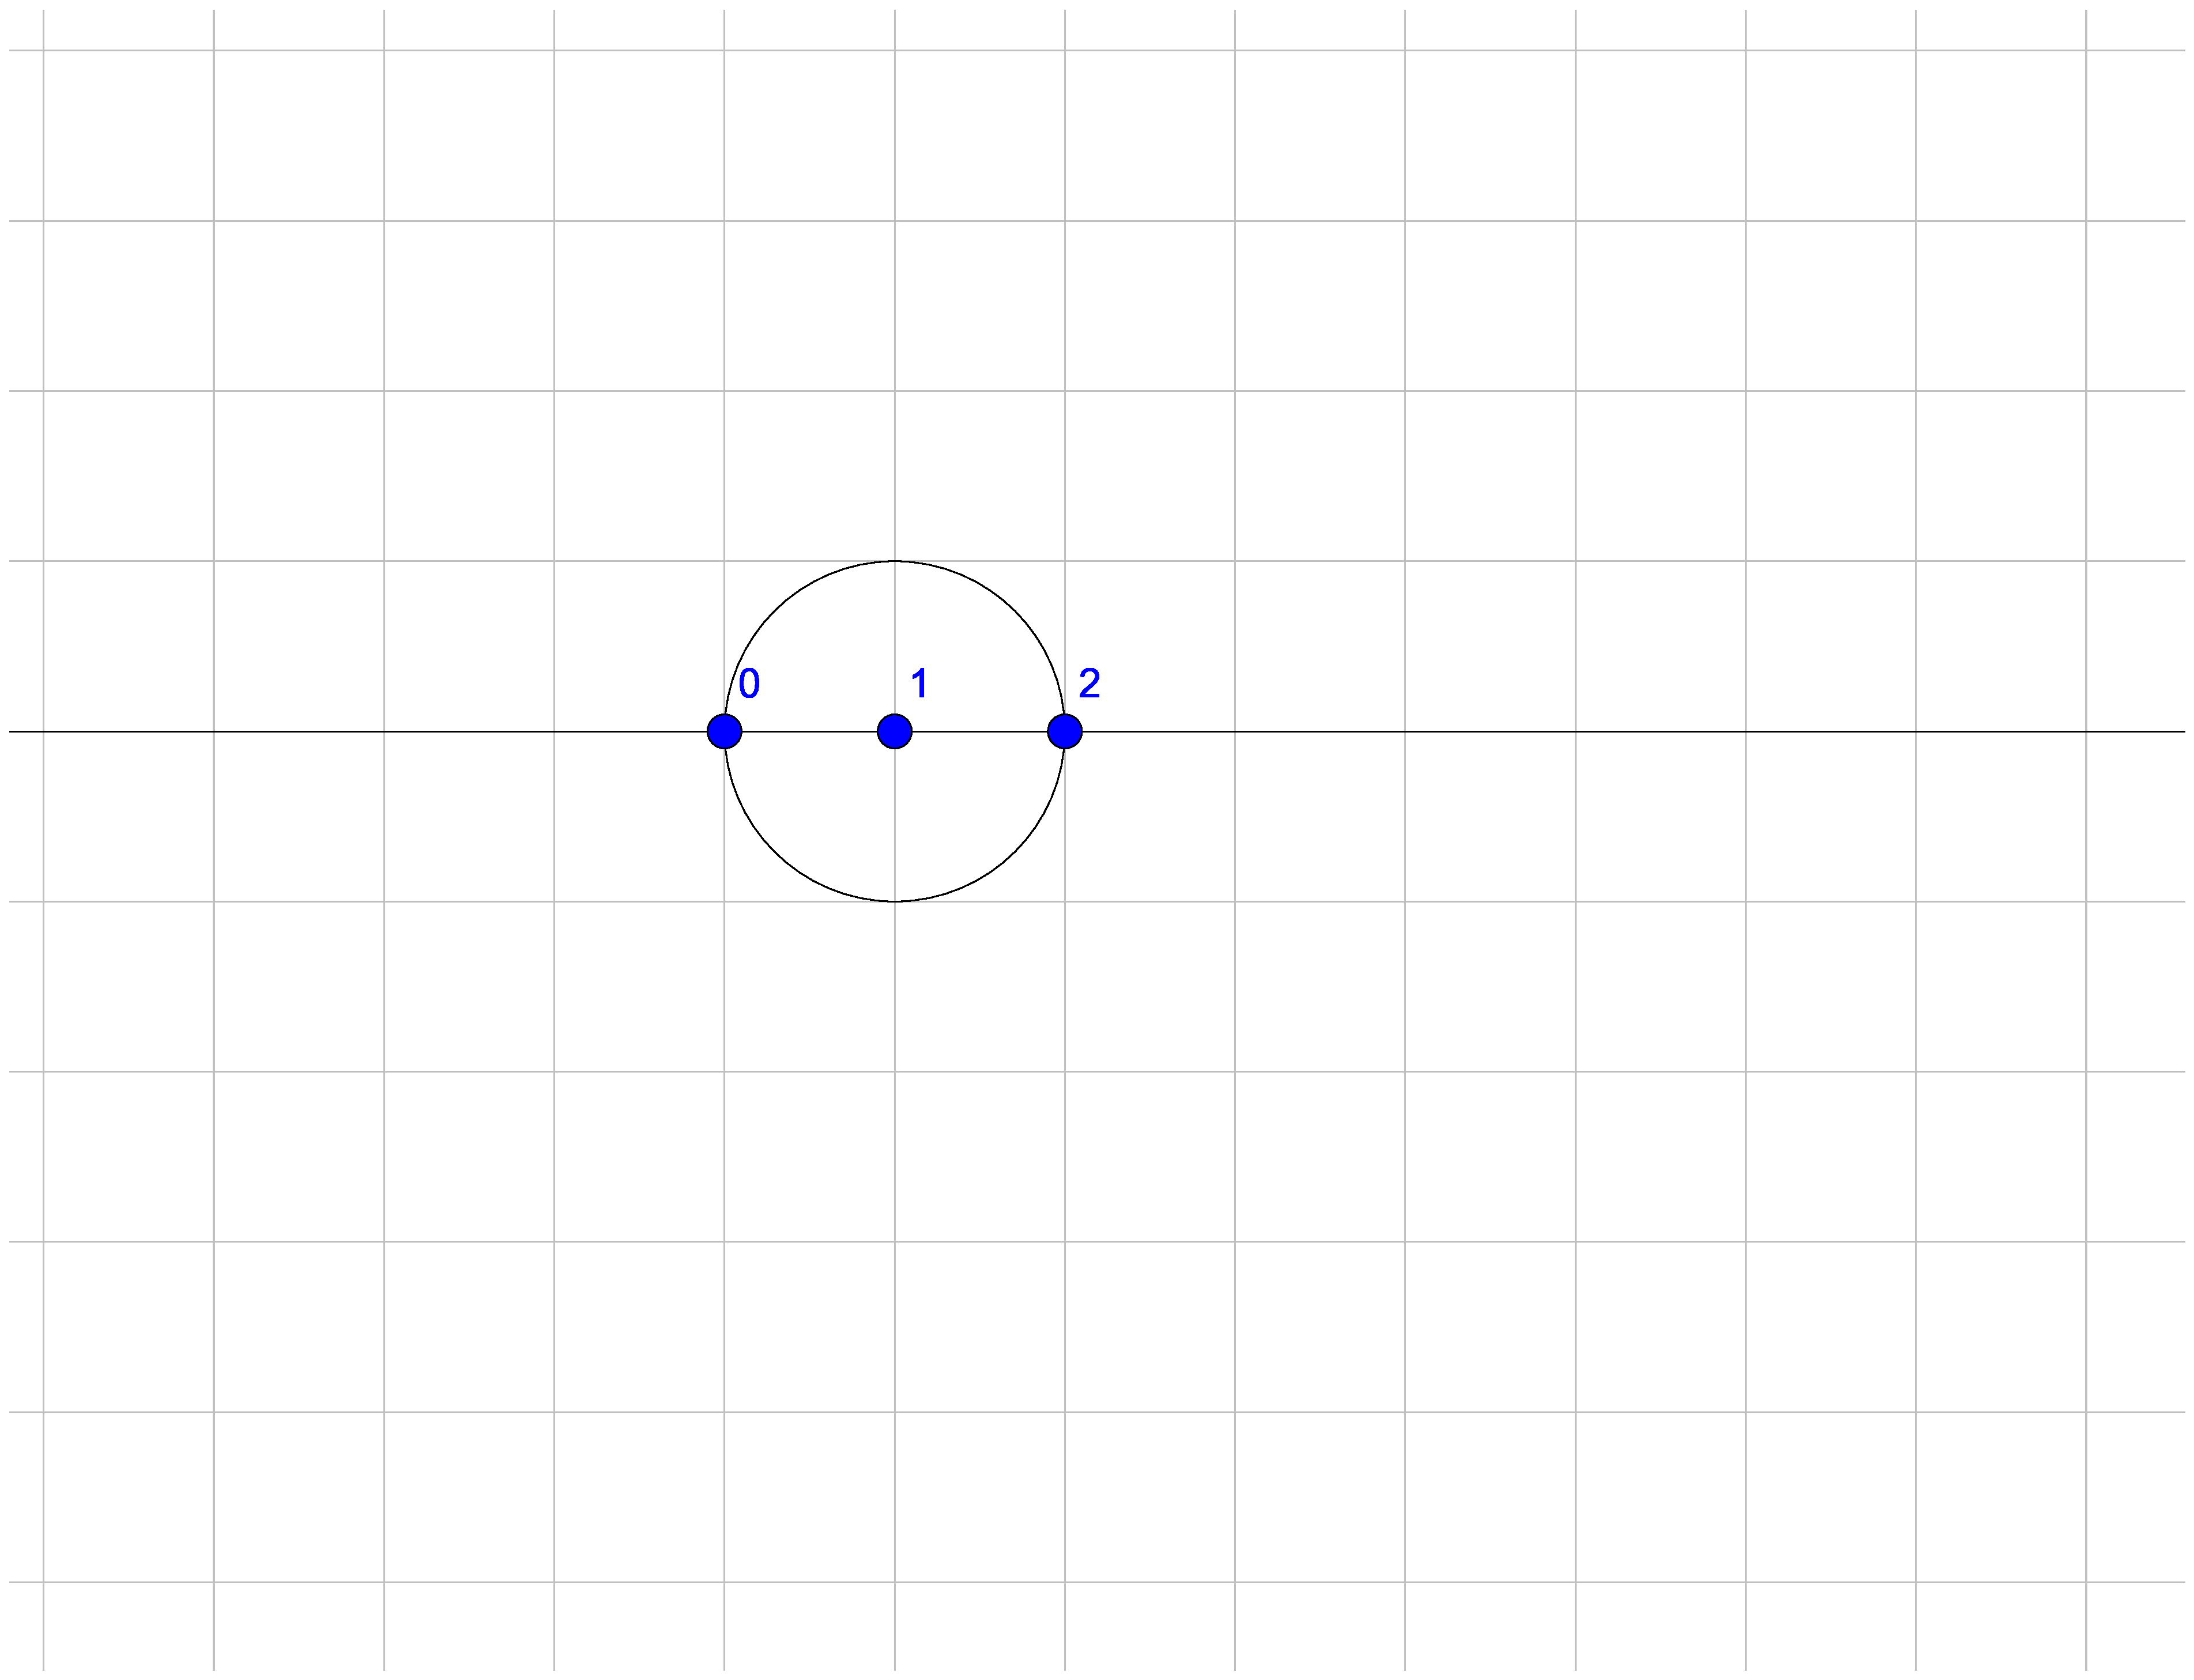
\includegraphics[scale=0.1]{ex25.eps}
\label{fig:ex2,5}
\end{figure}
\end{przyklad}
\end{frame}

\begin{frame}{Liczby Konstruowalne}
\begin{przyklad}
Liczby naturalne
\begin{figure}[!htb]
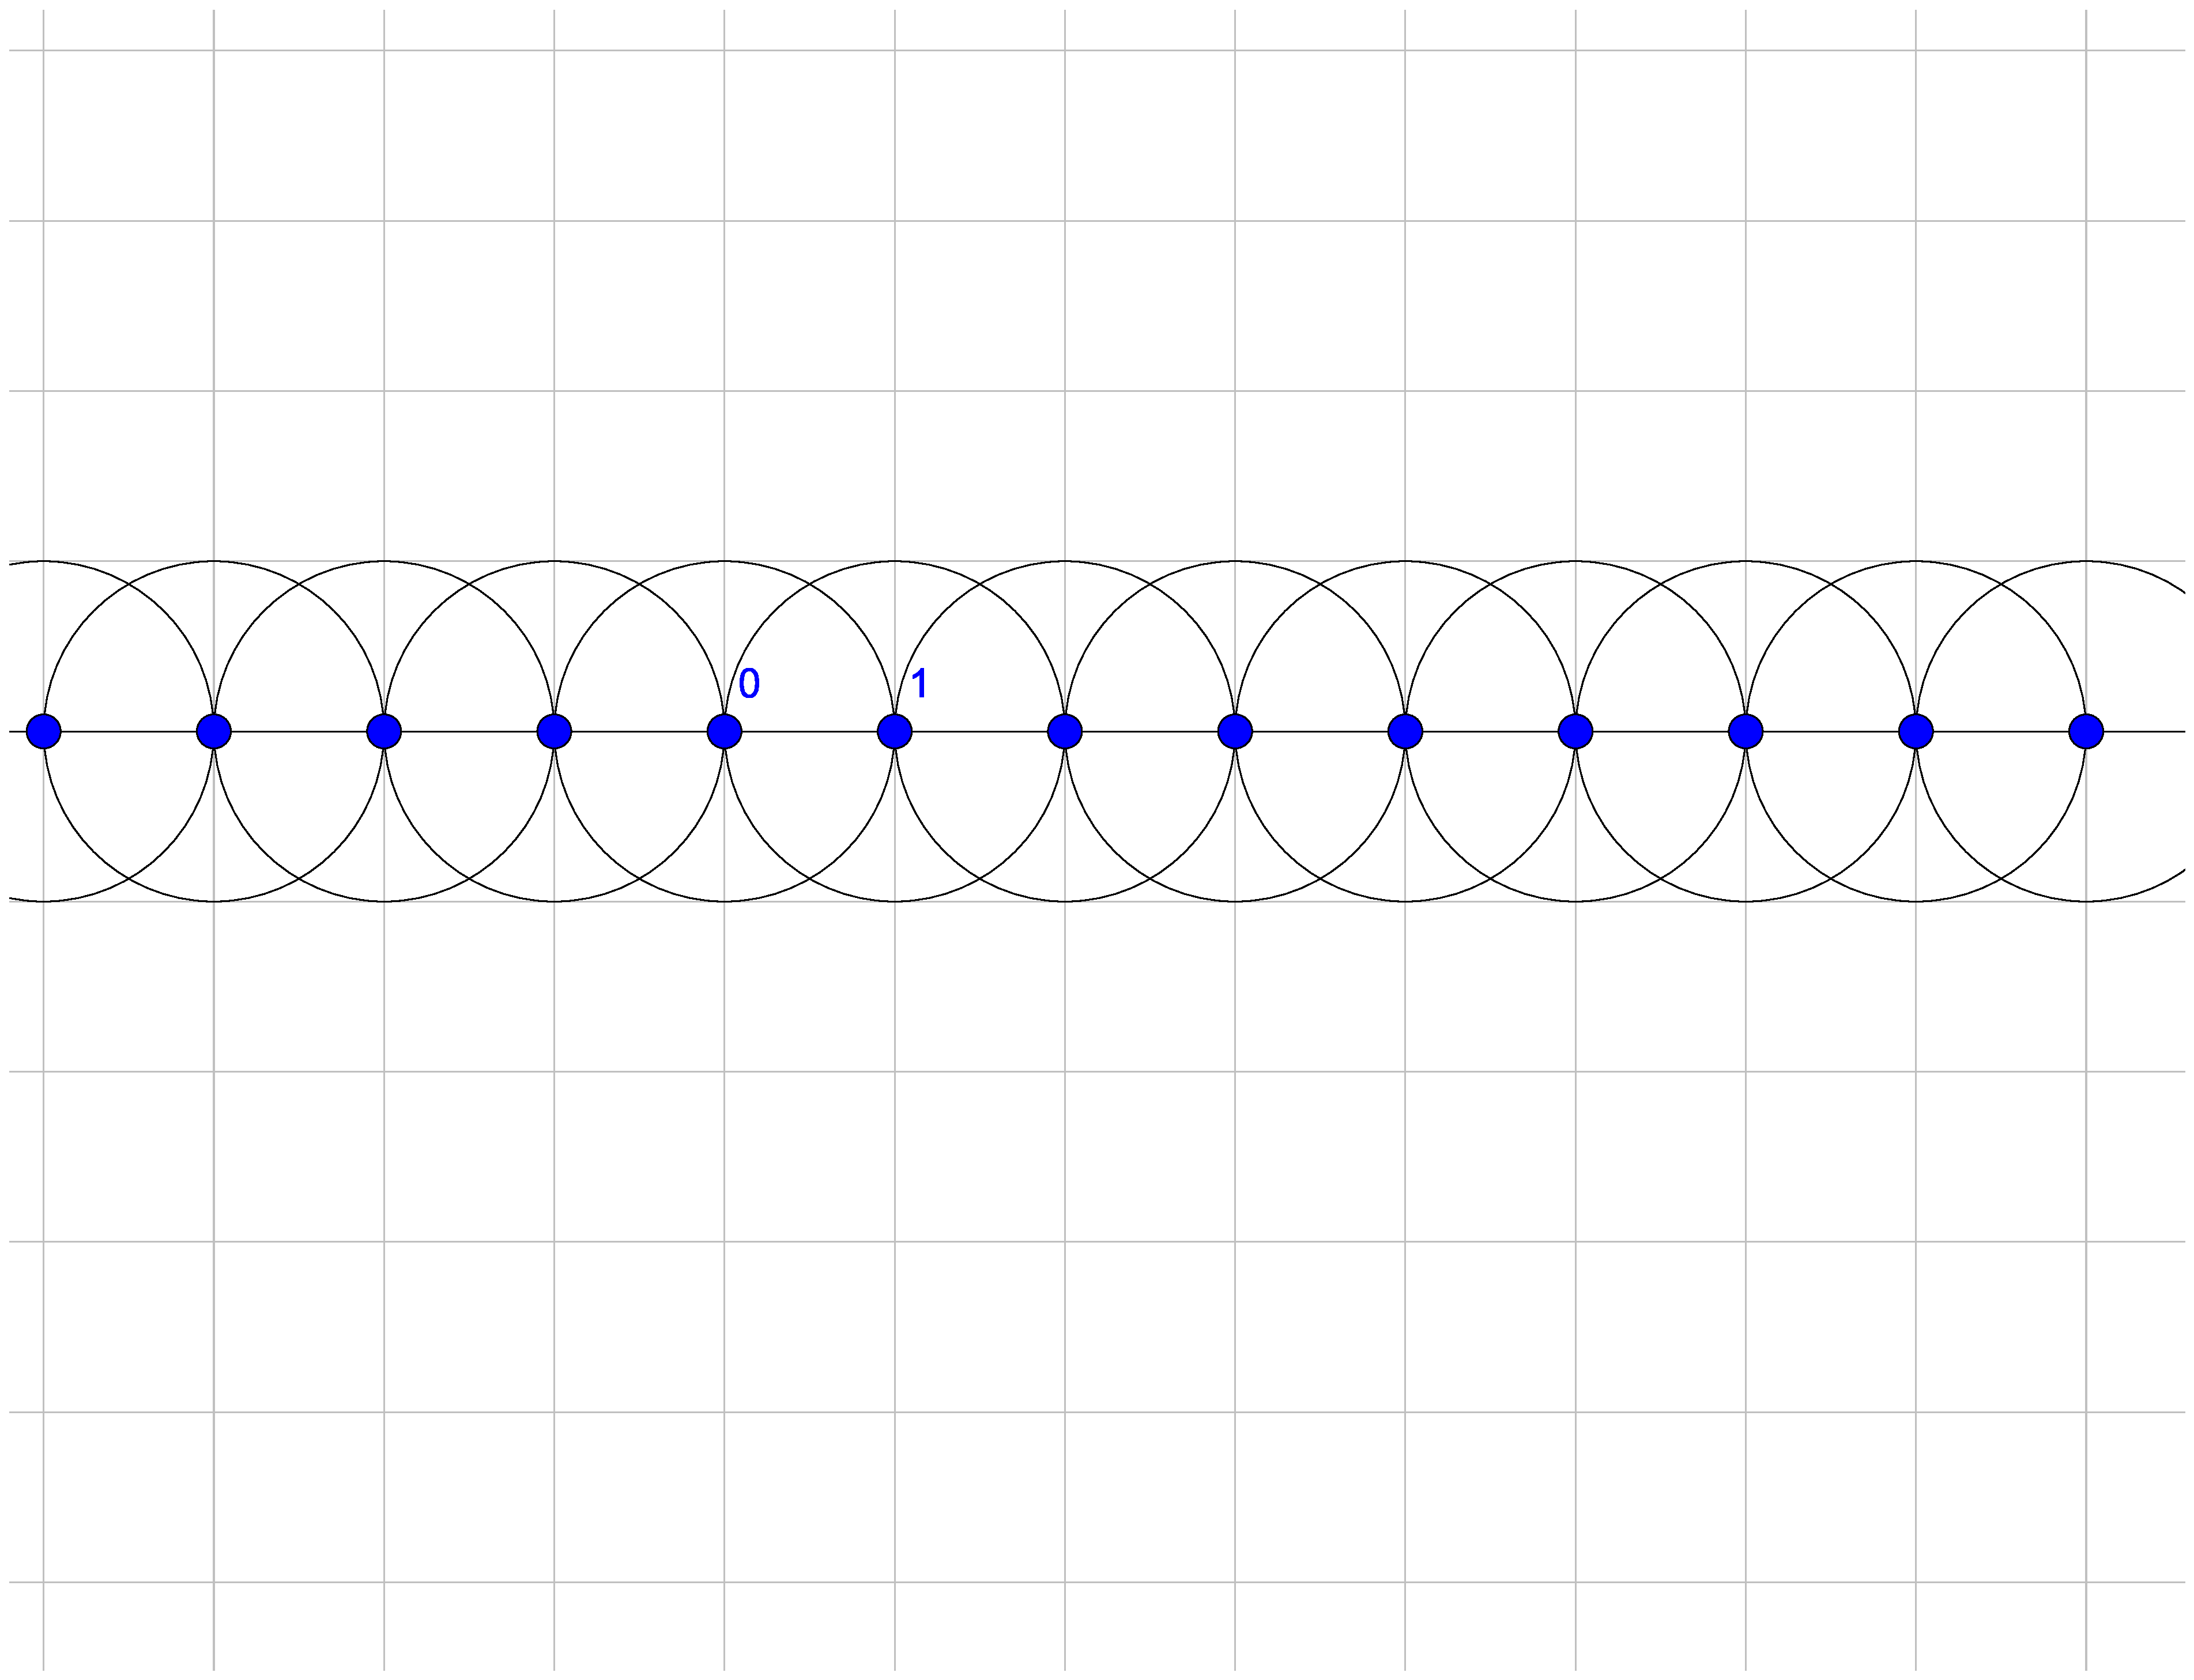
\includegraphics[scale=0.1]{ex3.eps}
\label{fig:ex3}
\end{figure}
\end{przyklad}
\end{frame}

\begin{frame}{Liczby Konstruowalne}
\begin{przyklad}
Liczby urojone całkowite
\begin{figure}[!htb]
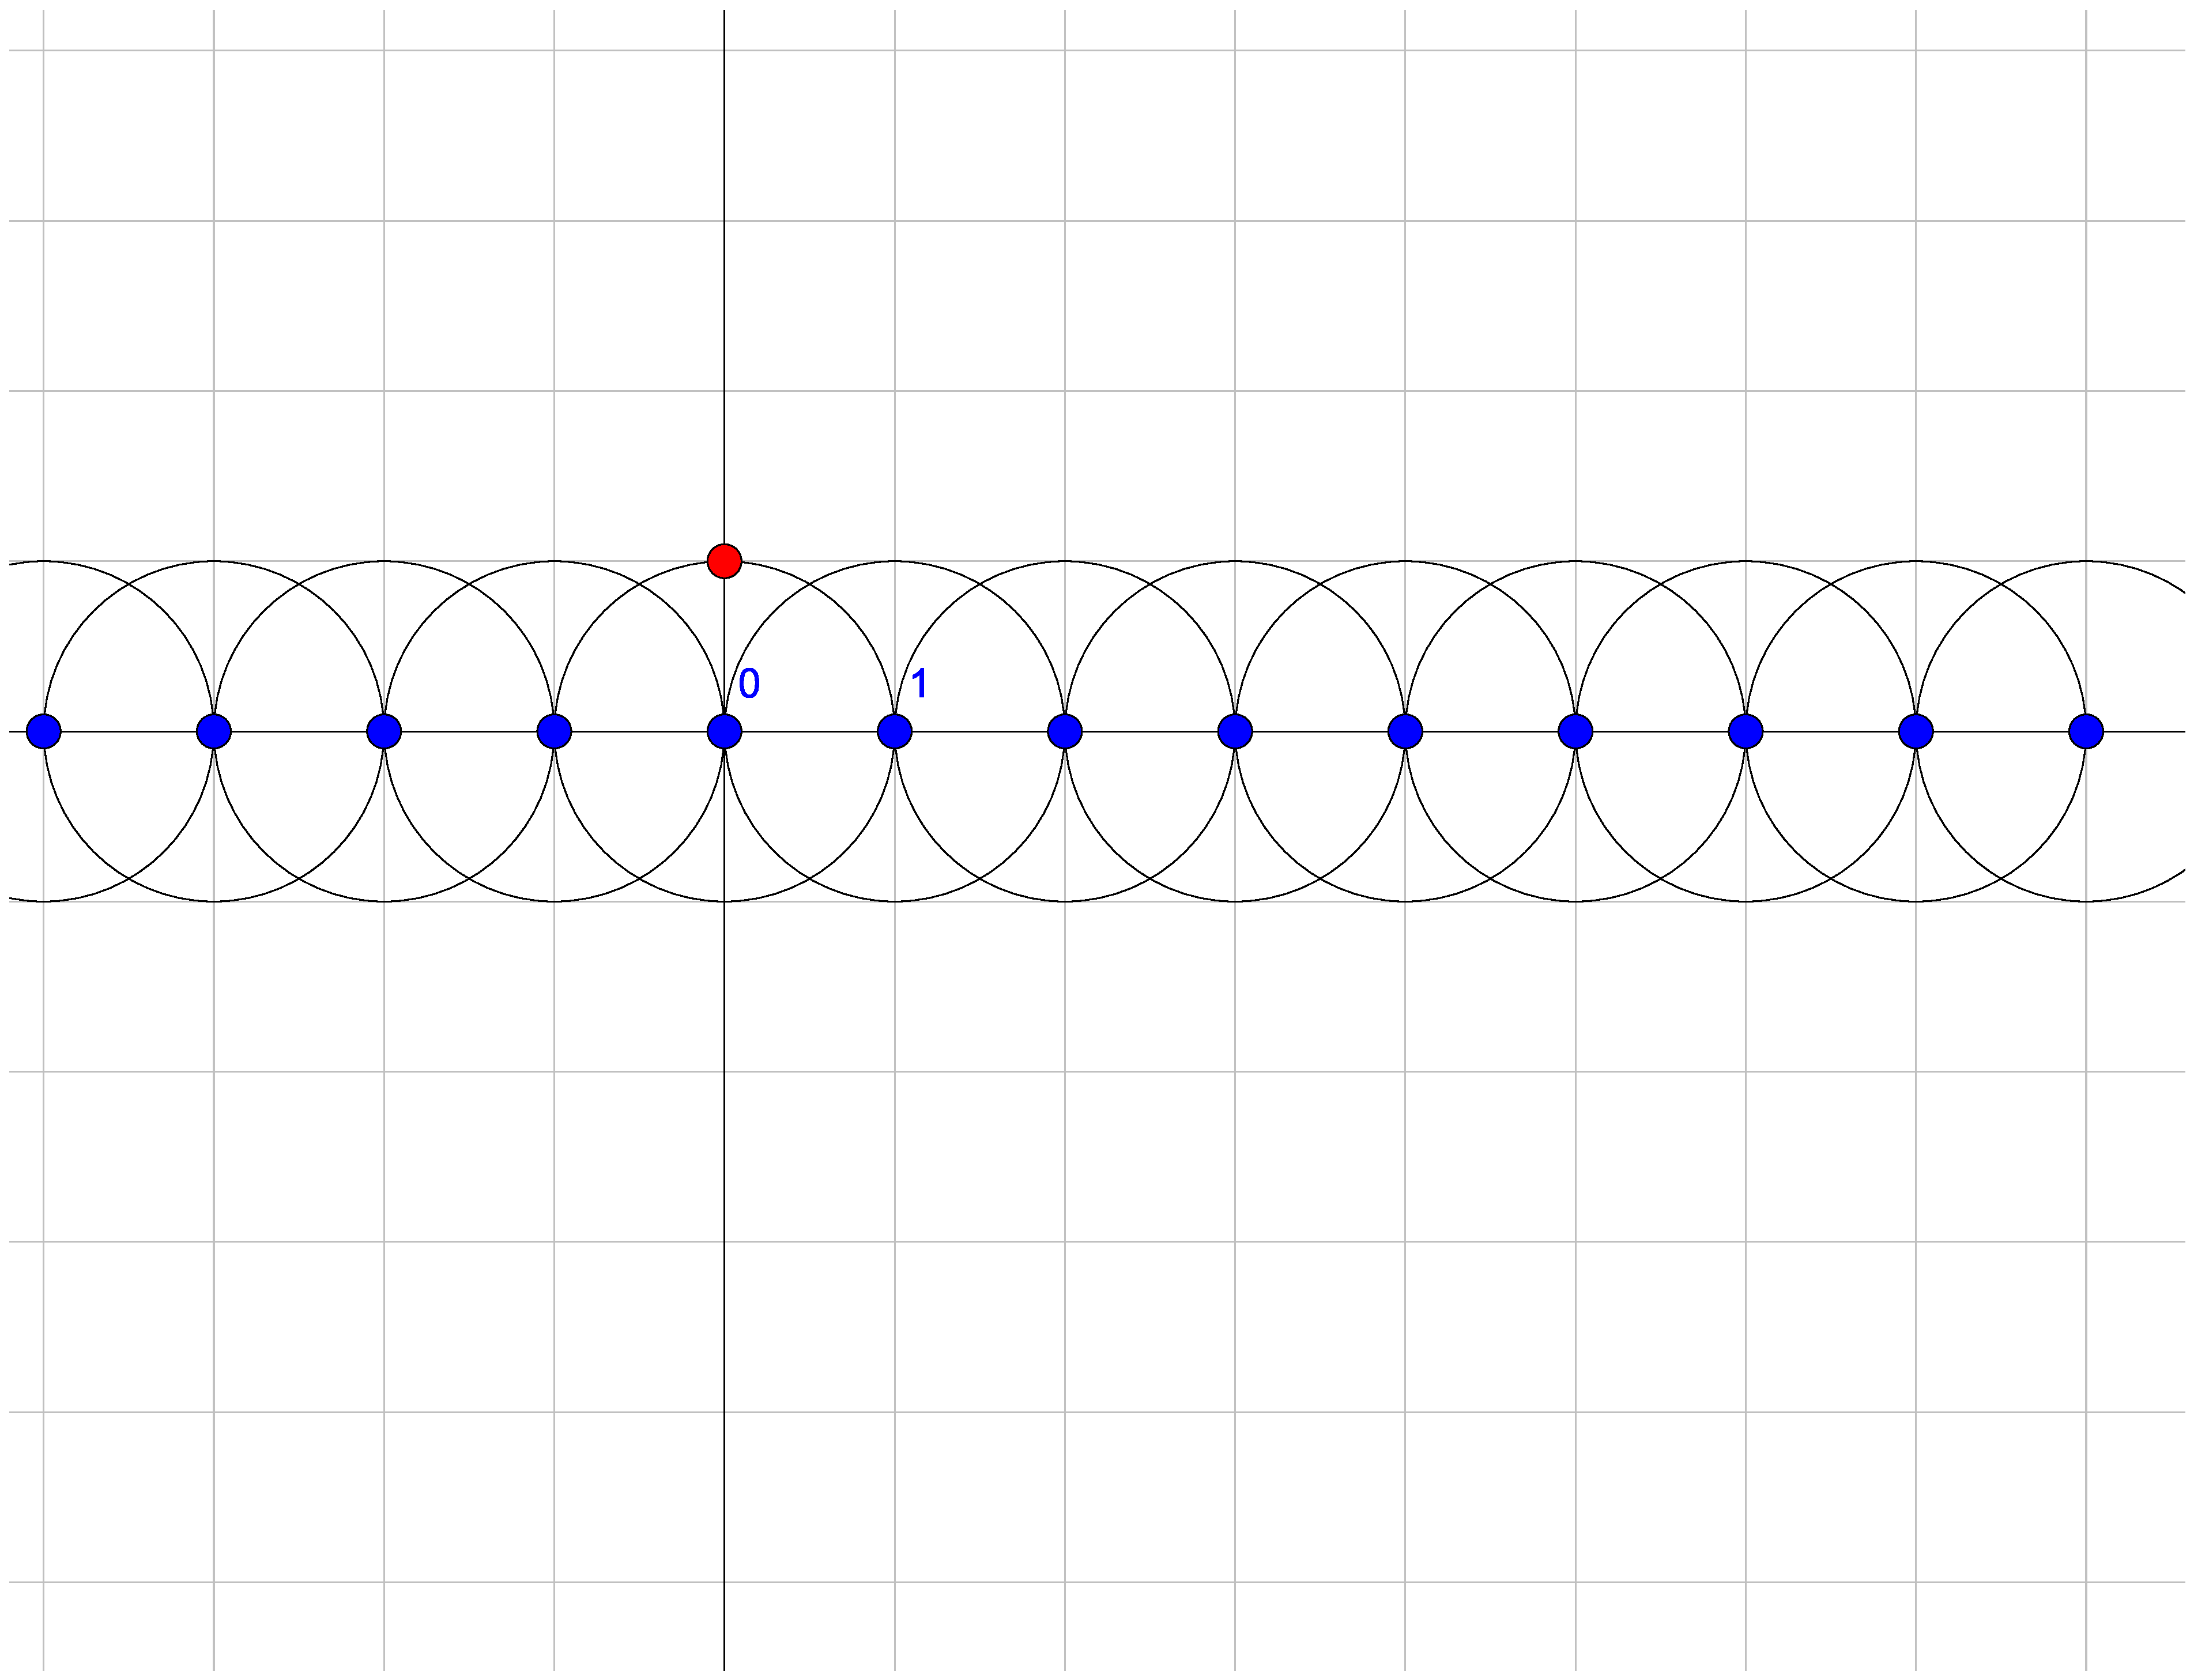
\includegraphics[scale=0.1]{ex4.eps}
\label{fig:ex4}
\end{figure}
\end{przyklad}
\end{frame}

\begin{frame}{Liczby Konstruowalne}
\begin{twierdzenie}
Niech $\mathcal{C}=\{\alpha\in\mathbb{C}\ |\ \alpha\ jest\ konstuowalne\}$. $\mathcal{C}$ jest podciałem 	$\mathbb{C}$ Ponadto: 
\begin{enumerate}[label=(\alph*)]
\item Niech $\alpha = a + bi\in\mathcal{C}$, gdzie $a,b\in\mathbb{R}$, to $a,b\in\mathcal{C}$.
\item Jeżeli $\alpha \in \mathcal{C}$, to $\sqrt{\alpha}\in\mathcal{C}$
\end{enumerate}
\end{twierdzenie}
\end{frame}

\begin{frame}{Liczby Konstruowalne}
\begin{figure}[!htb]
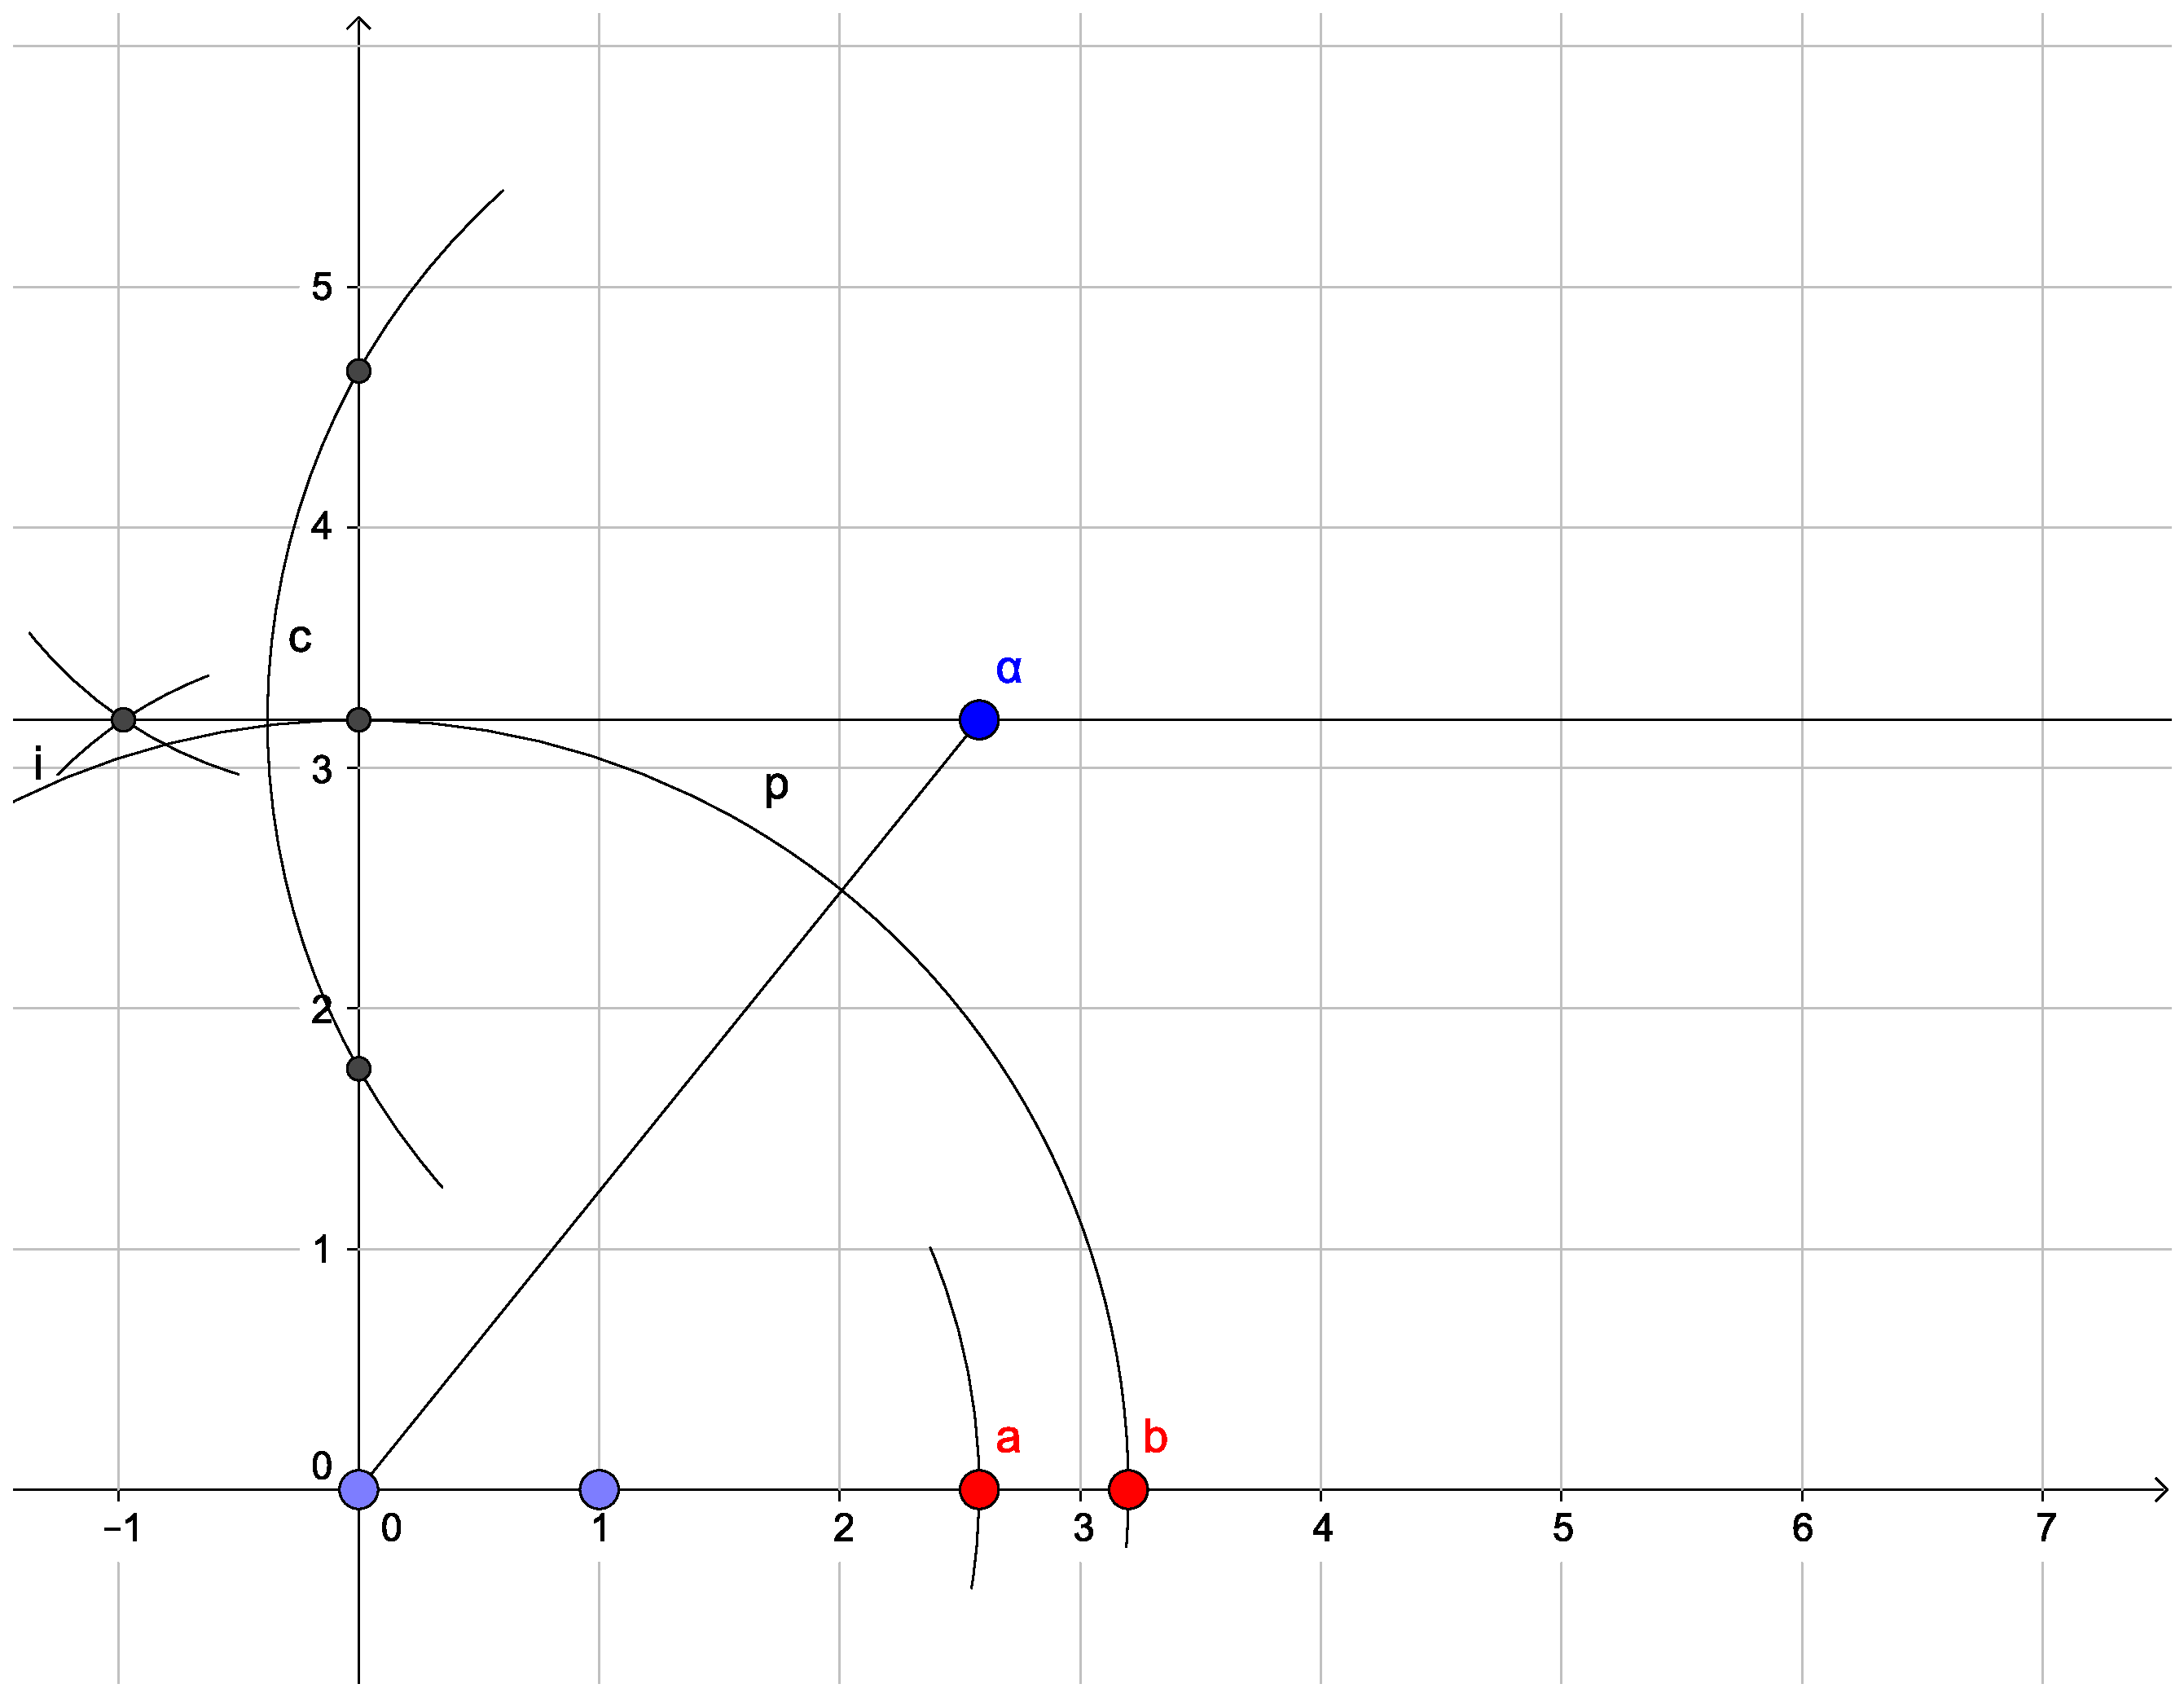
\includegraphics[scale=0.15]{wsp.eps}
\label{fig:dodawanie}
\end{figure}
\end{frame}

\begin{frame}{Liczby Konstruowalne}
\begin{figure}[!htb]
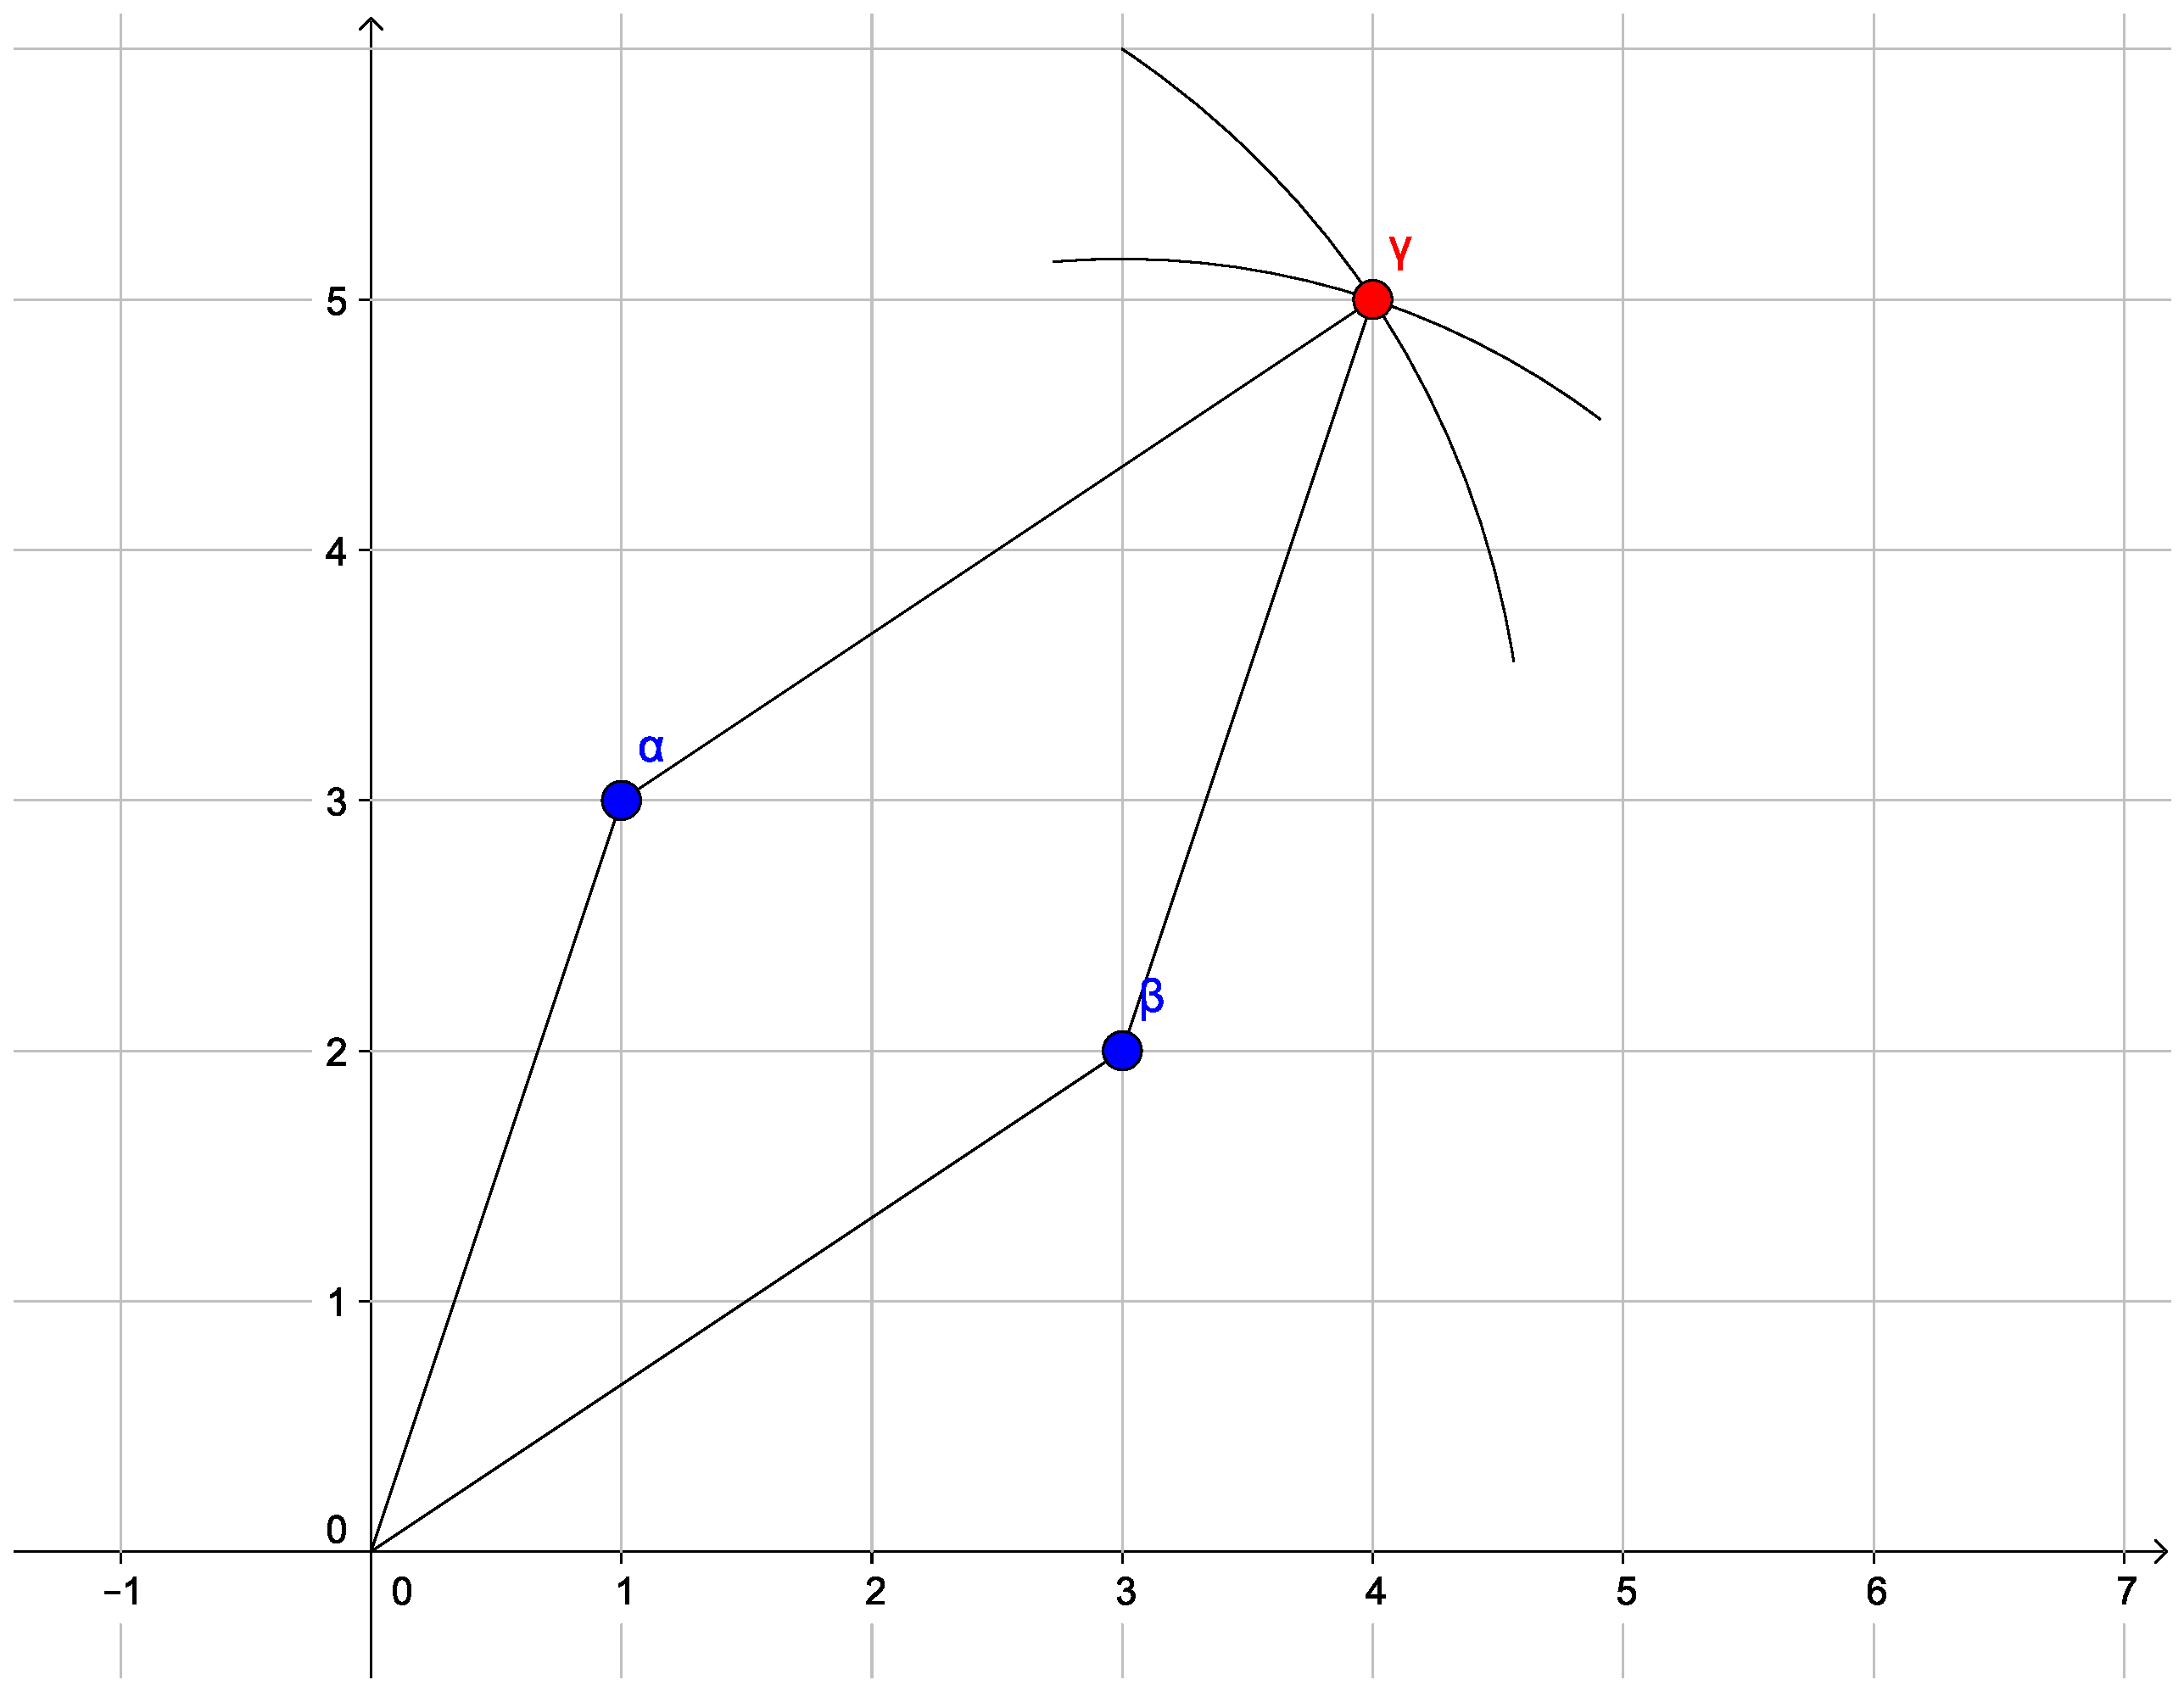
\includegraphics[scale=0.15]{suma.eps}
\label{fig:dodawanie}
\end{figure}
\end{frame}

\begin{frame}{Liczby Konstruowalne}
\begin{Huge}
$$\alpha \cdot \beta=ae^{\theta} \cdot be^{\tau}=(ab)e^{\theta+\tau}$$
\end{Huge}
\end{frame}

\begin{frame}{Liczby Konstruowalne}
\begin{figure}[!htb]
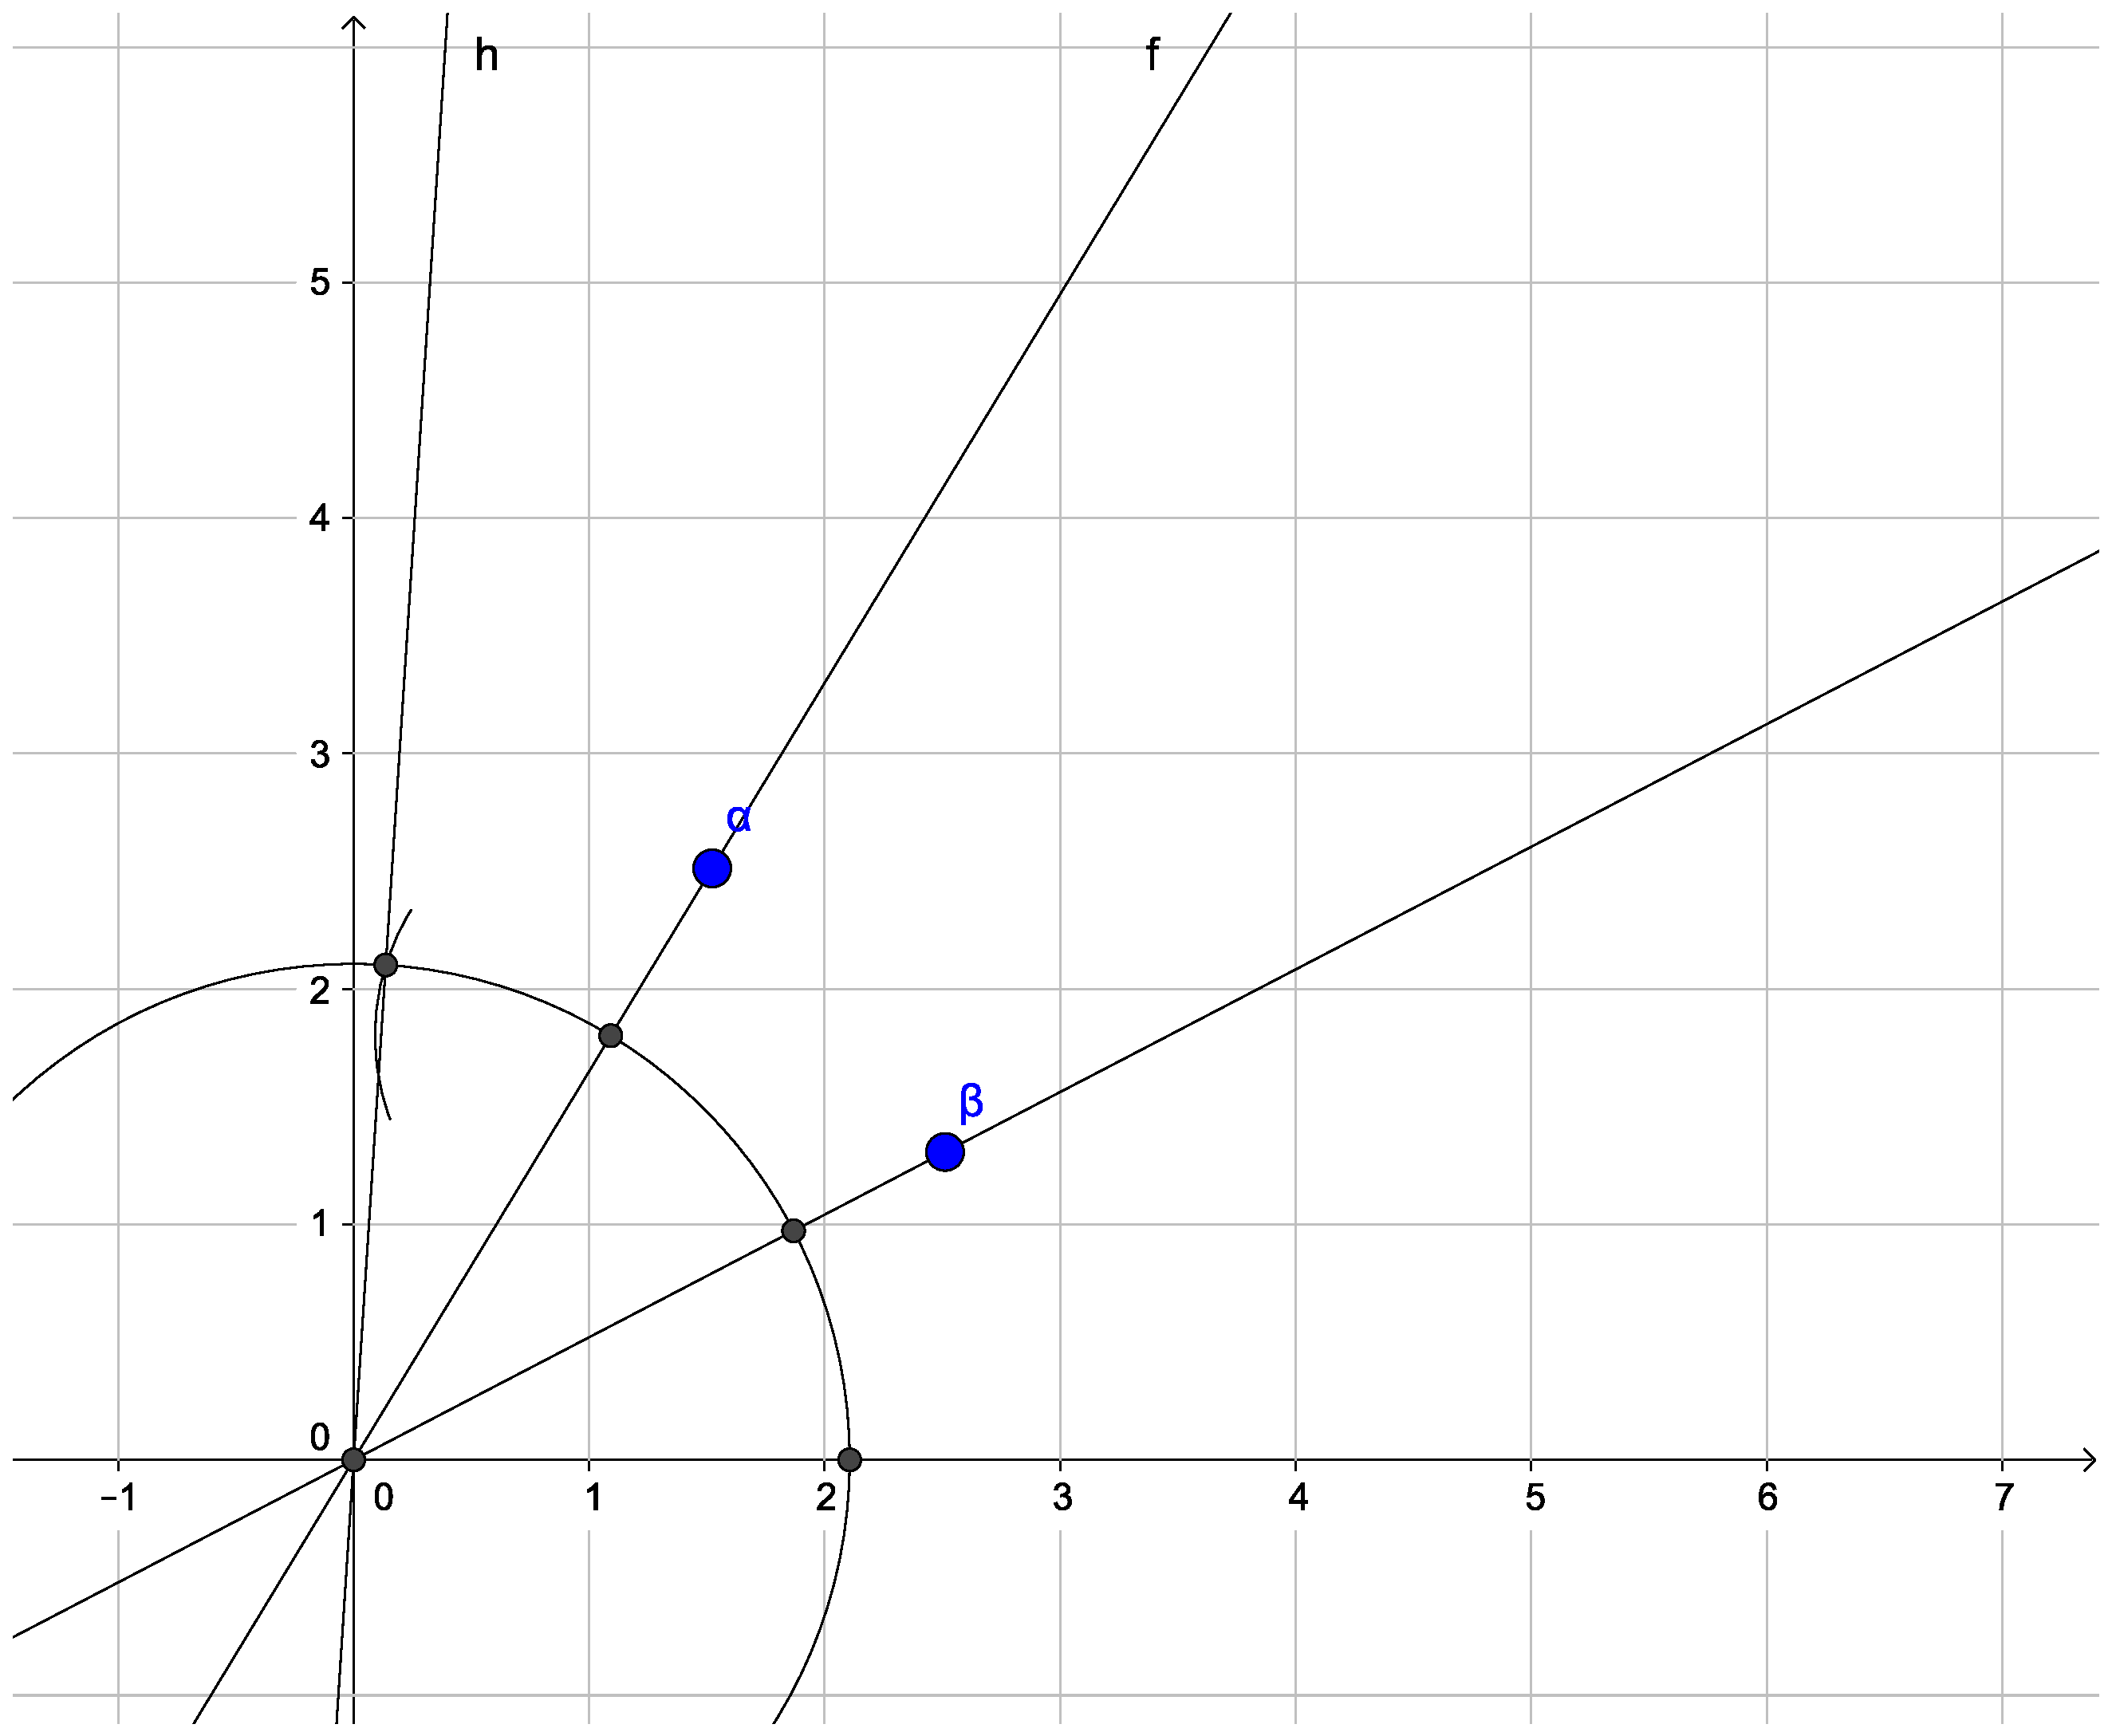
\includegraphics[scale=0.15]{iloczyn1.eps}
\label{fig:iloczyn1}
\end{figure}
\end{frame}

\begin{frame}{Liczby Konstruowalne}
\begin{figure}[!htb]
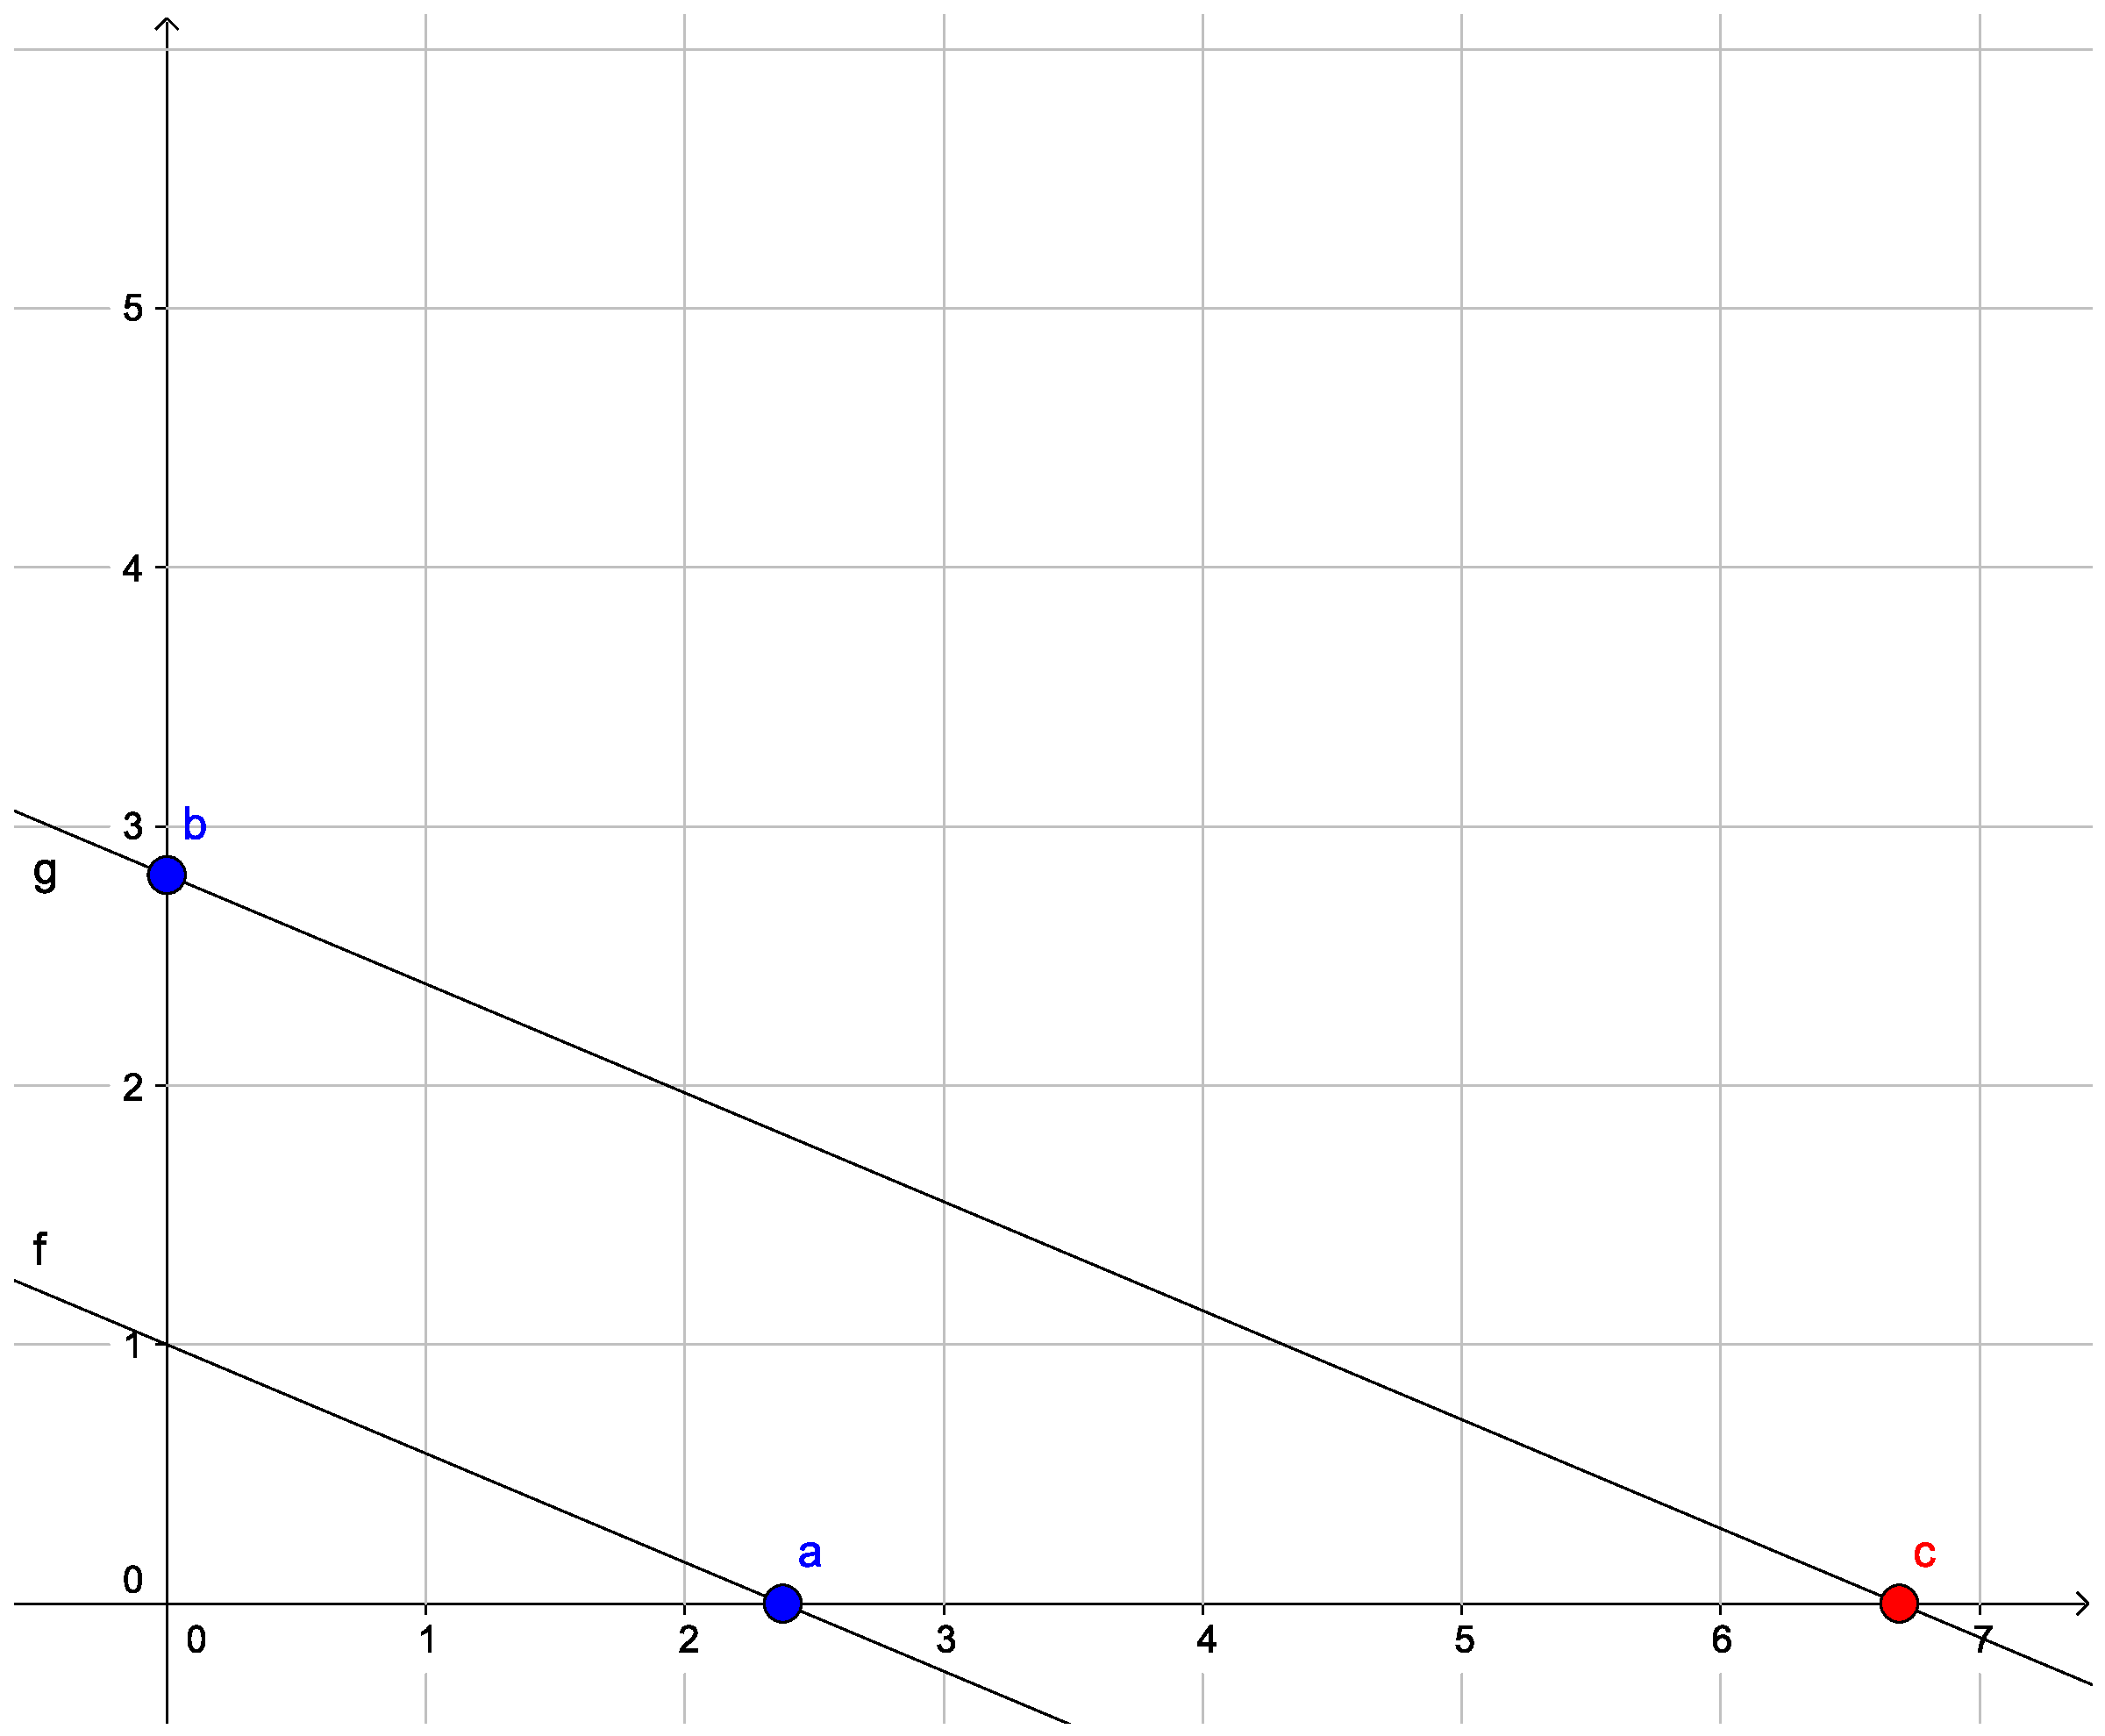
\includegraphics[scale=0.15]{iloczyn2.eps}
\label{fig:iloczyn2}
\end{figure}
\end{frame}

\begin{frame}{Liczby Konstruowalne}
\begin{Huge}
$$\frac{\alpha}{\beta}=\frac{ae^{\theta}}{be^{\tau}}=(\frac{a}{b})e^{\theta-\tau}$$
\end{Huge}
\end{frame}

\begin{frame}{Liczby Konstruowalne}
\begin{figure}[!htb]
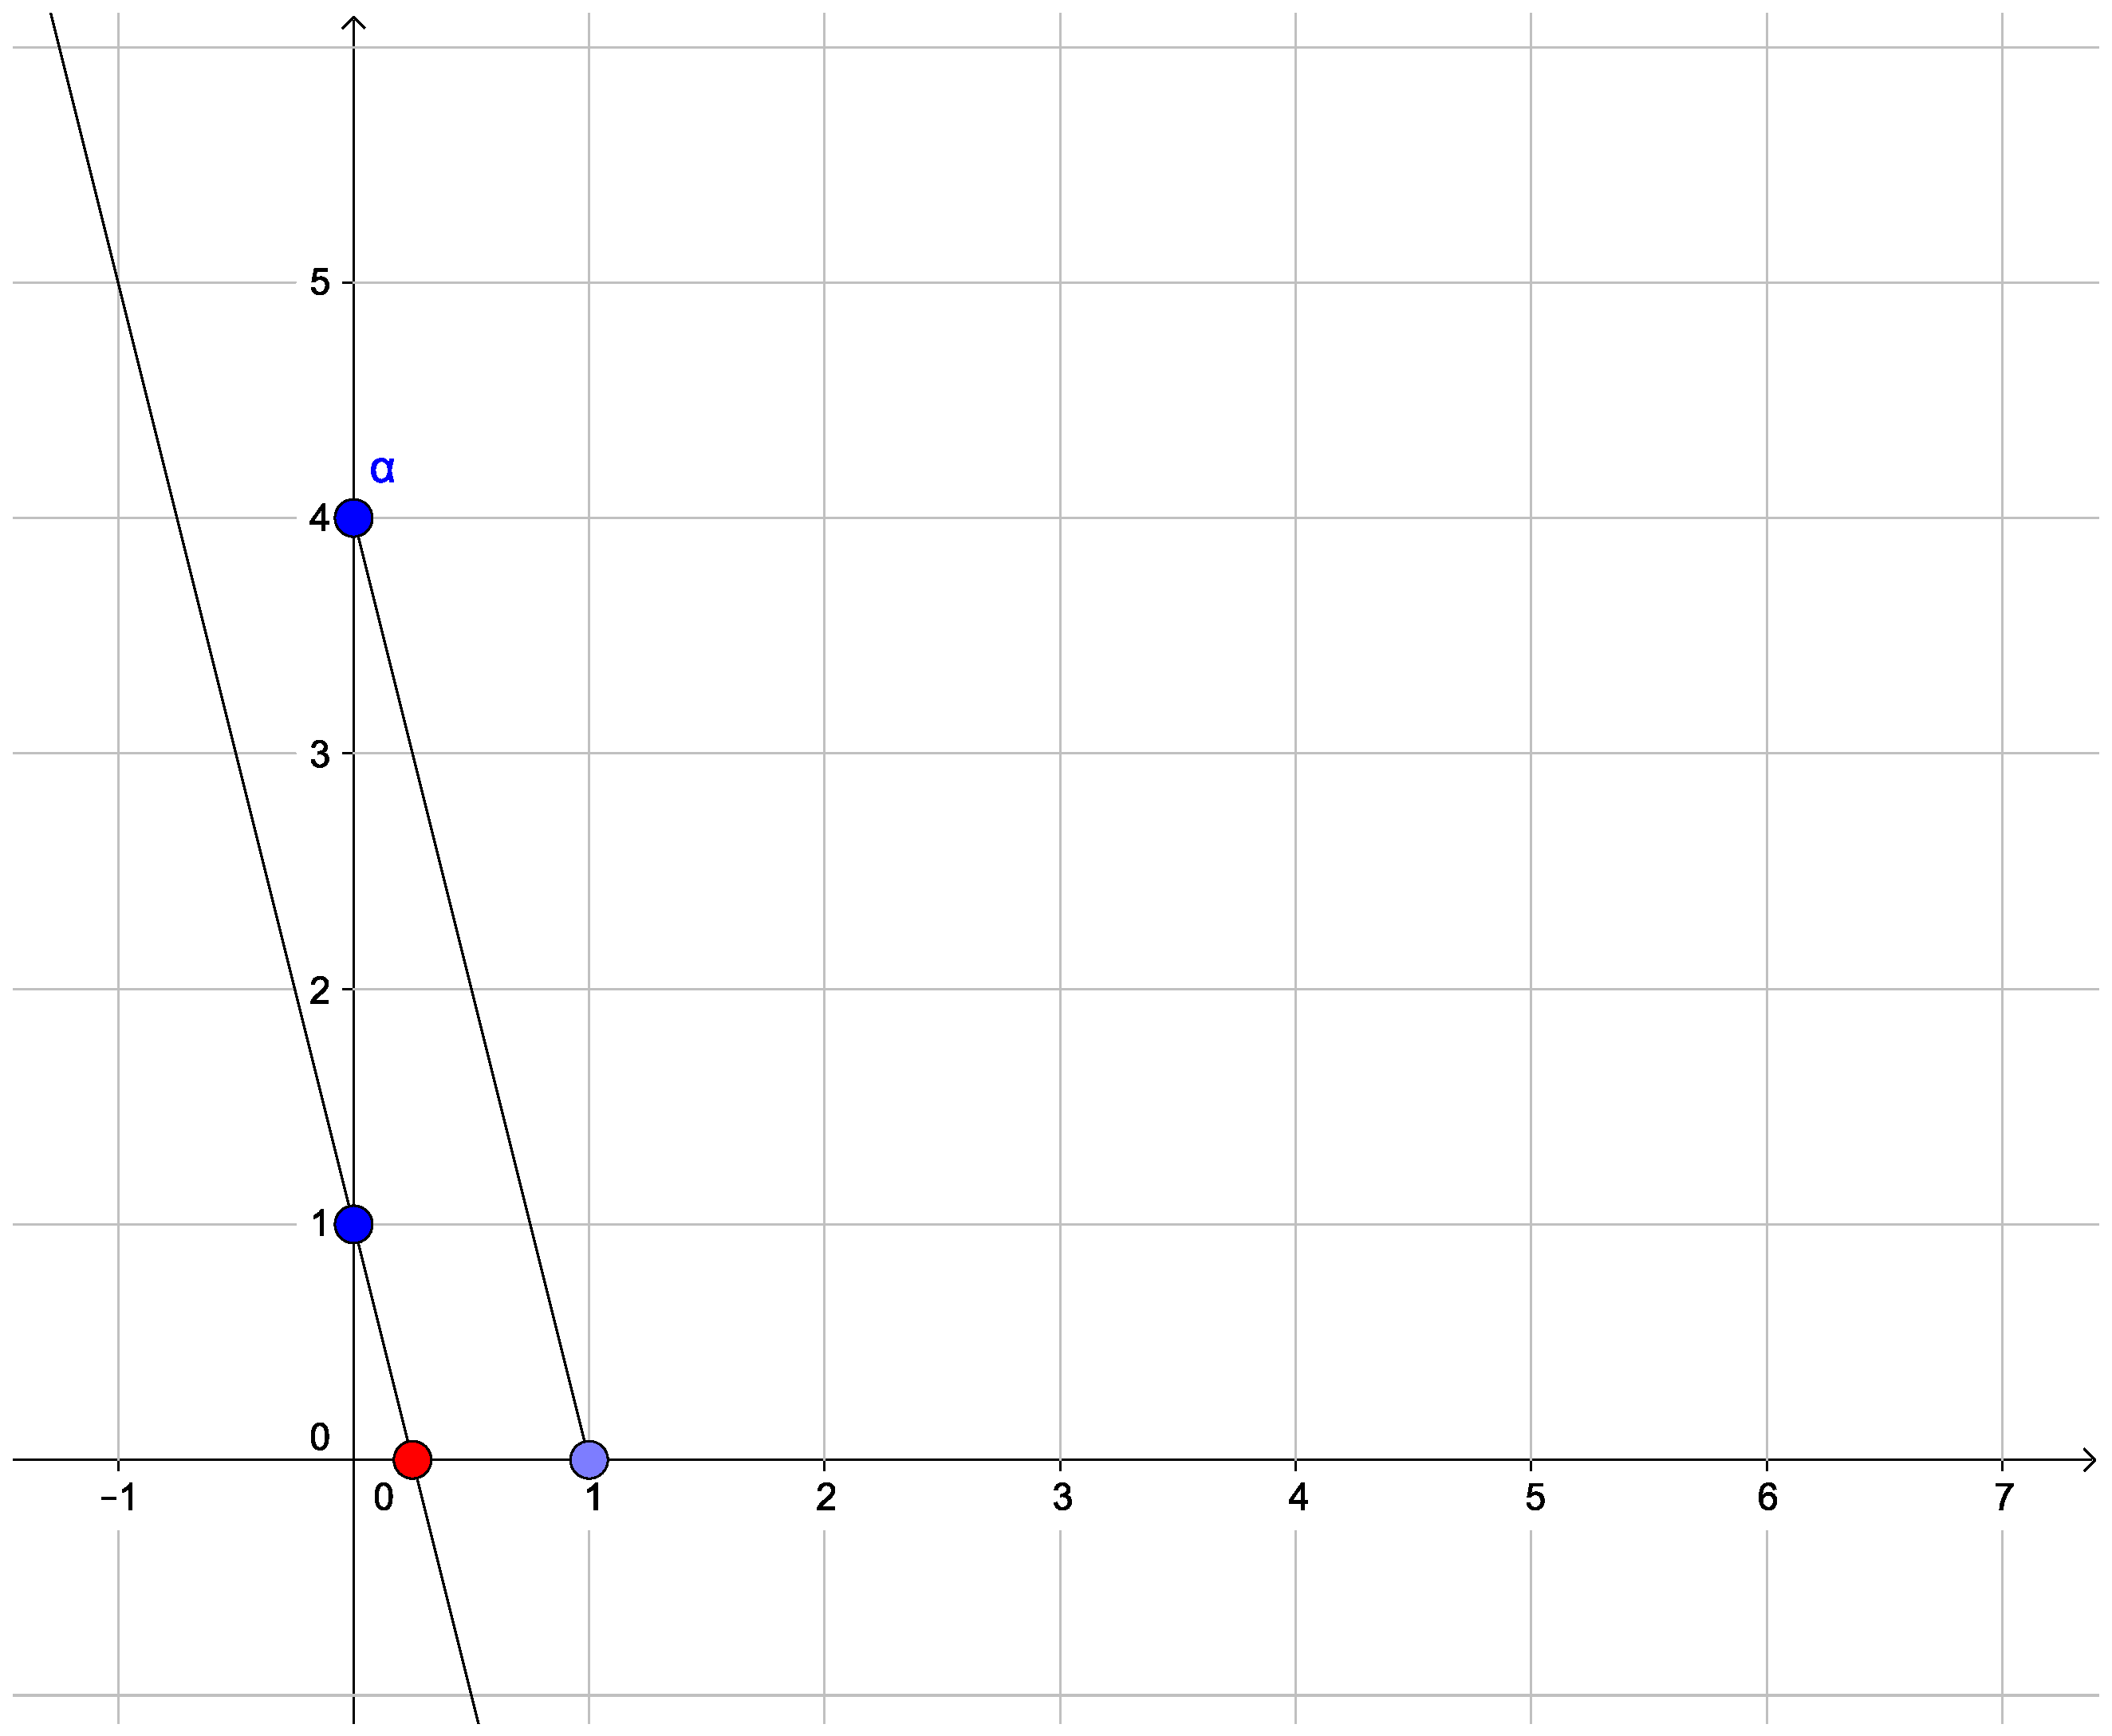
\includegraphics[scale=0.15]{iloraz.eps}
\label{fig:iloraz}
\end{figure}
\end{frame}

\begin{frame}{Liczby Konstruowalne}
\begin{Huge}
$$\sqrt{\alpha}=\sqrt{r}e^{\frac{\theta}{2}}$$
\end{Huge}
\end{frame}

\begin{frame}{Liczby Konstruowalne}
\begin{figure}[!htb]
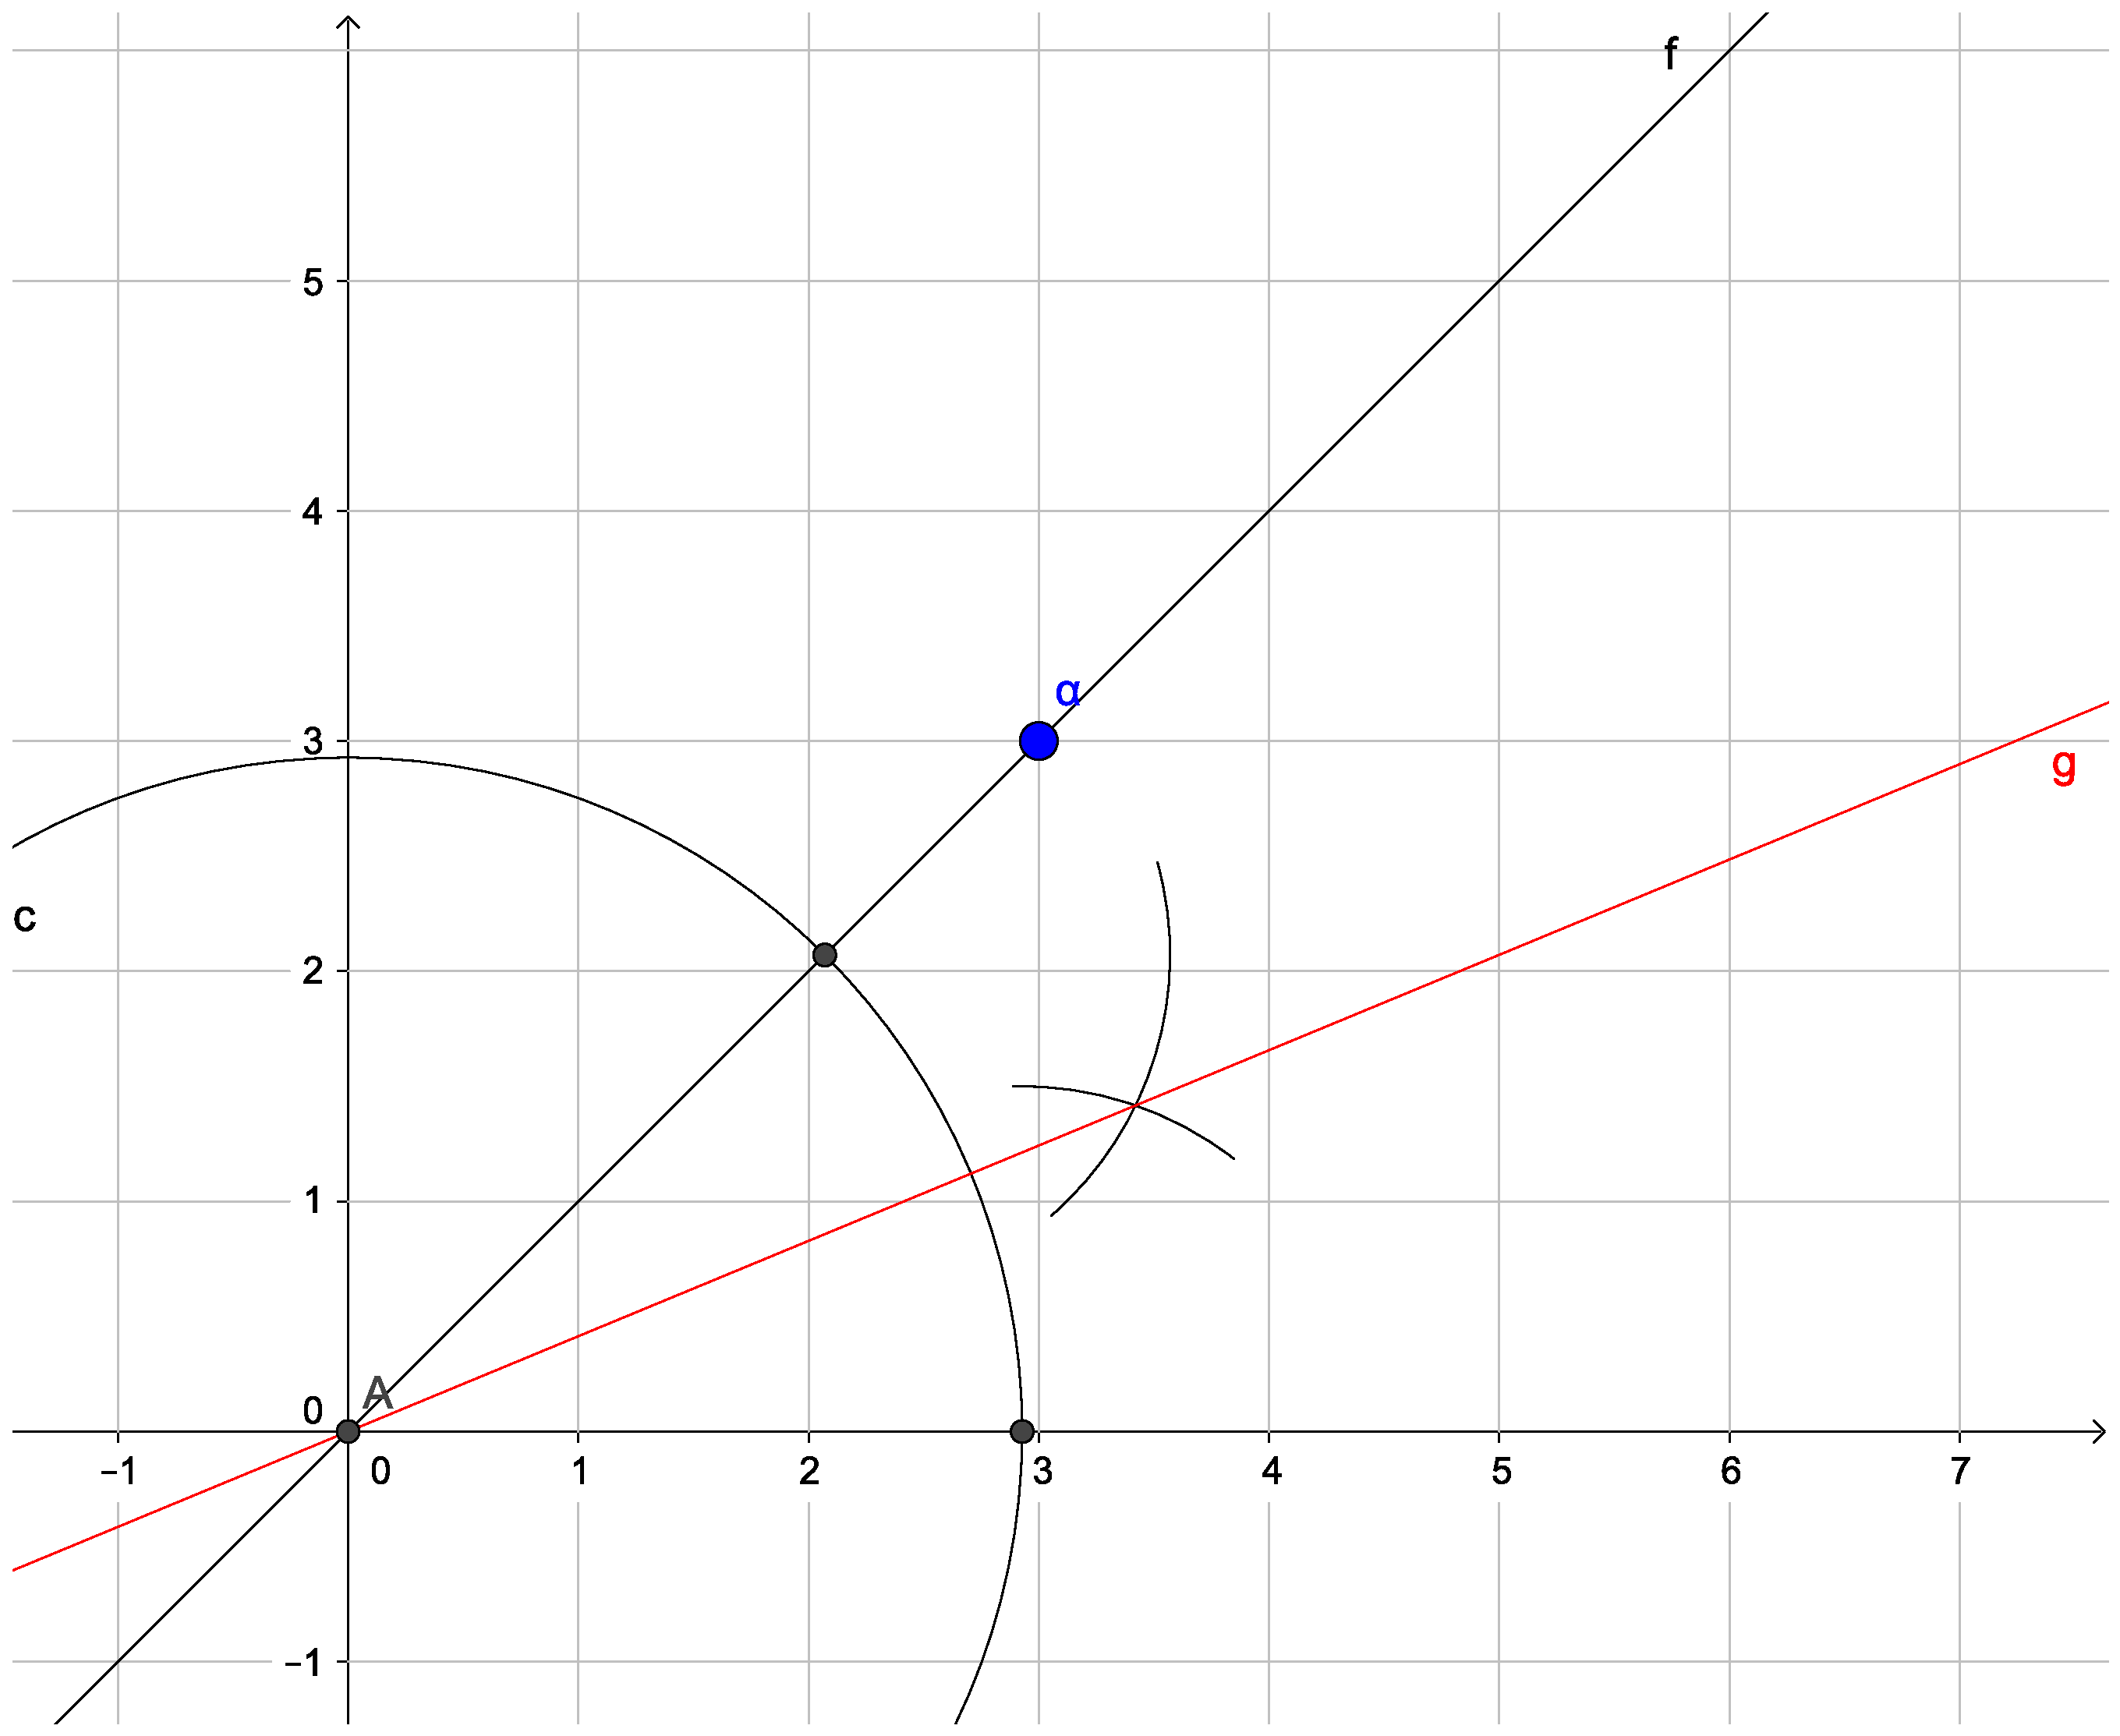
\includegraphics[scale=0.15]{pierwiastek1.eps}
\label{fig:pierwiastek1}
\end{figure}
\end{frame}


\begin{frame}{Liczby Konstruowalne}
\begin{figure}[!htb]
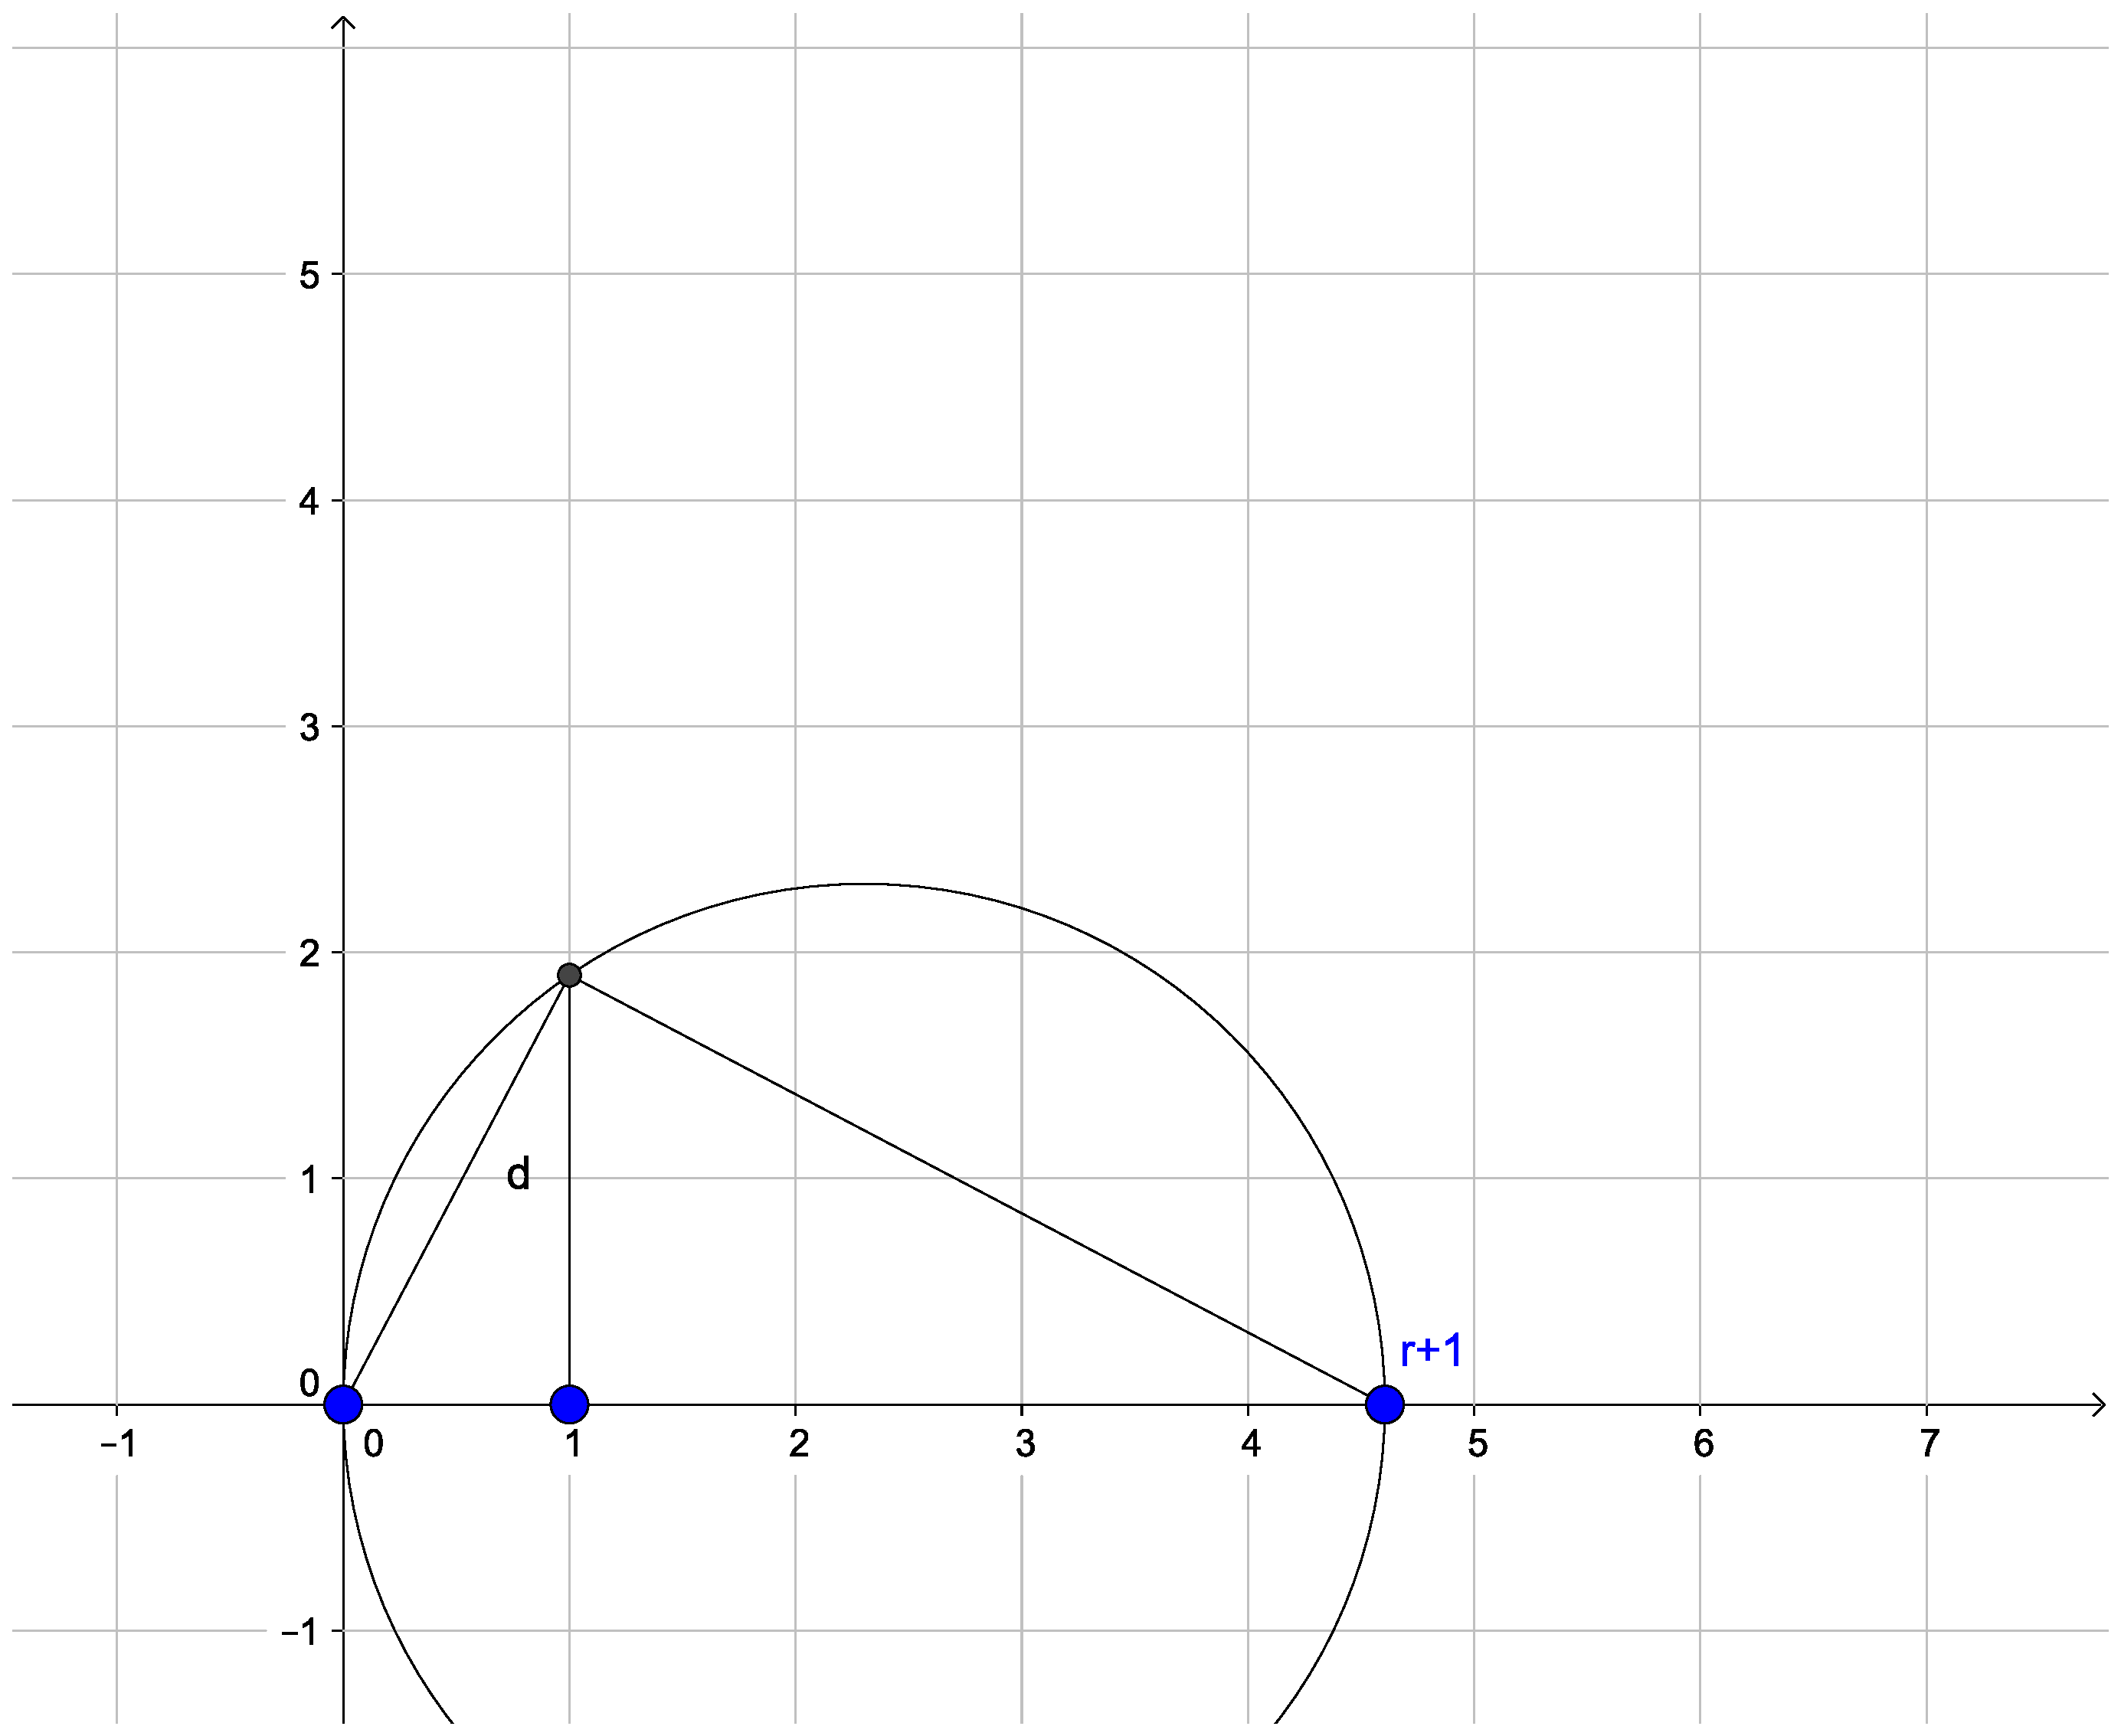
\includegraphics[scale=0.15]{pierwiastek2.eps}
\label{fig:pierwiastek1}
\end{figure}
\end{frame}

\begin{frame}{Przypomnienie}
\end{frame}

\begin{frame}{Liczby Konstruowalne}
\begin{twierdzenie}\label{wieza}
Niech $\alpha$ będzie liczbą zespoloną. Wtedy $\alpha\in\mathcal{C}$ wtedy i tylko wtedy, gdy istnieją ciała $$\mathbb{Q}=F_0 \subset F_1 \subset ...\subset F_n \subset \mathbb{C}$$ takie, że $\alpha\in F_n$ i $[F_{i-1}:F_i]=2$ dla $0<i\leqslant n$ 
\end{twierdzenie}
\end{frame}


\begin{frame}{Liczby Konstruowalne}
\begin{proofs}
($\Leftarrow$) Załóżmy, że istnieje $\mathbb{Q}=F_0 \subset ...\subset F_n \subset \mathbb{C}$ gdzie $[F_{i-1}:F_i]=2$. Możemy skorzystać z faktu, że jeżeli $[F_{i-1}:F_i]=2$, to $F_i=F_{i-1}(\sqrt{\alpha_i})$ dla pewnego $\alpha_i\in F_{i-1}$. Poprzez indukcję udowodnimy, że dla $0<i\leqslant n$ $F_i\subset \mathbb{Q}$. Oczywiście $F_0=\mathbb{Q}\subset\mathcal{C}$. Załóżmy, że $F_{i-1}\subset \mathcal{C}$, $F_i=F_{i-1}(\sqrt{\alpha_i})$ . Skoro $\alpha_i\in\mathcal{C}$, to $\sqrt{\alpha_i}\in\mathcal{C}$, stąd $F_i=F_{i-1}(\sqrt{\alpha_i})\in\mathcal{C}$. Zatem $F_n\in\mathcal{C}$.
\end{proofs}
\end{frame}

\begin{frame}{Liczby Konstruowalne}
\begin{proofs}
($\Rightarrow$) $\alpha\in\mathcal{C}$ Udowodnimy, przez stworzenie wieży rozszerzeń
$\mathbb{Q}=F_0 \subset F_1 \subset ...\subset F_n \subset \mathbb{C}$ gdzie $[F_{i-1}:F_i]=2$ takie, że $F_n$ wartości urojone i rzeczywiste liczb, które powstają w trakcie konstrukcji $\alpha$. Przeprowadzimy indukcje po liczbie $N$ użyć aksjomatów P1, P2, P3.
Dla $N=0$ $\alpha=0$ lub $\alpha=1$ zatem $\mathbb{Q}=F_0=F_n$.
\end{proofs}
\end{frame}

\begin{frame}{Liczby Konstruowalne}
\begin{proofs}
Niech $N>1$ i punkt $\alpha$ został otrzymany za pomocą P1, przecięcie się prostych $l_1$, $l_2$. Proste powstały z punktów $\alpha_1$ i $\beta_1$ oraz $\alpha_2$ i $\beta_2$. 
$\alpha_1$, $\beta_1$, $\alpha_2$, $\beta_2$ powstały w co najwyżej $N-1$ krokach, zatem z założenia indukcyjnego istnieje $\mathbb{Q}=F_0 \subset F_1 \subset ...\subset F_n \subset \mathbb{C}$ gdzie $[F_{i-1}:F_i]=2$, że części urojone i rzeczywiste $\alpha_1$, $\beta_1$, $\alpha_2$, $\beta_2$ należą do $F_n$. Prosta $l_1$ jest opisana równaniem $a_1 x+b_1 y=c_1$, ponieważ $\alpha_1,\beta_1\in F_n$ to $a_1,b_1,c_1\in F_n$. analogicznie równaniem $l_2$ jest $a_2 x+b_2 y=c_2$. $\alpha$ jest punktem przecięcia się $l_1$, $l_2$. Zatem jego części urojone i rzeczywiste rozwiązaniem układu równań:
\begin{equation*}
\begin{matrix}
a_1 x+b_1 y=c_1\\
a_2 x+b_2 y=c_2
\end{matrix}
\end{equation*}
Stąd $\alpha\in F_n$
\end{proofs}
\end{frame}

\begin{frame}{Liczby Konstruowalne}
\begin{proofs}
Niech $N>1$ i punkt $\alpha$ został otrzymany za pomocą P1, przecięcie się prostych $l_1$, $l_2$. Proste powstały z punktów $\alpha_1$ i $\beta_1$ oraz $\alpha_2$ i $\beta_2$. 
$\alpha_1$, $\beta_1$, $\alpha_2$, $\beta_2$ powstały w co najwyżej $N-1$ krokach, zatem z założenia indukcyjnego istnieje $\mathbb{Q}=F_0 \subset F_1 \subset ...\subset F_n \subset \mathbb{C}$ gdzie $[F_{i-1}:F_i]=2$, że części urojone i rzeczywiste $\alpha_1$, $\beta_1$, $\alpha_2$, $\beta_2$ należą do $F_n$. Prosta $l_1$ jest opisana równaniem $a_1 x+b_1 y=c_1$, ponieważ $\alpha_1,\beta_1\in F_n$ to $a_1,b_1,c_1\in F_n$. analogicznie równaniem $l_2$ jest $a_2 x+b_2 y=c_2$. $\alpha$ jest punktem przecięcia się $l_1$, $l_2$. Zatem jego części urojone i rzeczywiste rozwiązaniem układu równań:
\begin{equation*}
\begin{matrix}
a_1 x+b_1 y=c_1\\
a_2 x+b_2 y=c_2
\end{matrix}
\end{equation*}
Stąd $\alpha\in F_n$
\end{proofs}
\end{frame}

\begin{frame}{Liczby Konstruowalne}
\begin{proofs}
Niech $N>1$ i punkt $\alpha$ został otrzymany za pomocą P2, przecięcie się prostej $l$ i okręgu $o$. Jak poprzednio można znaleźć $\mathbb{Q}=F_0 \subset F_1 \subset ...\subset F_n \subset \mathbb{C}$ gdzie $[F_{i-1}:F_i]=2$, że części rzeczywiste i urojone punktów, z których powstały $l$ i $o$, należą do $F_n$.\\
 $\alpha$ jest rozwiązaniem układu równań.
\begin{equation*}
\begin{matrix}
a_1x+b_1 y=c_1\\
x^2+y^2+a_2x+b_2y+c_2=0
\end{matrix}
\end{equation*}
Gdzie $a_1,b_1,a_2,b_2,c_2\in F_n$. Załóżmy, że $a_1\not =0$, więc możemy przyjąć, że $a_1=1$.Po podstawieniu $x=-b_1y+c_1$ otrzymujemy równanie kwadratowe:
$$(-b_1y+c_1)^2+y^2+a_2(-b_1y+c_1)+b_2y+c_2=0$$
\end{proofs}
\end{frame}

\begin{frame}{Liczby Konstruowalne}
\begin{proofs}
$$(-b_1y+c_1)^2+y^2+a_2(-b_1y+c_1)+b_2y+c_2=0$$
W przypadku, gdy wartości $y$, będące rozwiązaniami równania, należą do $F_n$, to $x=b_1y+c_1$ także należy do $F_n$, więc $F_n$ jest szukanym ciałem

Gdy rozwiązania nie należą do $F_n$, to istnieje rozszerzenie $F_{n+1}$ stopnia drugiego $F_n$, do którego należą wartości rozwiązania, $x=b_1y-c_1$ także należy do $F_{n+1}$. Zatem $F_{n+1}$ jest szukanym ciałem. 
\end{proofs}
\end{frame}

\begin{frame}{Liczby Konstruowalne}
\begin{proof}
Niech $N>1$ i punkt $\alpha$ został otrzymany za pomocą P3, przecięcie się dwóch okręgów $o_1$ i $o_2$. Jak poprzednio $\alpha$ jest rozwiązaniem równania
\begin{equation*}
\begin{matrix}
x^2+y^2+a_1x+b_1y+c_1=0\\
x^2+y^2+a_2x+b_2y+c_2=0
\end{matrix}
\end{equation*}
Po odjęciu stronami otrzymujemy:
\begin{equation*}
\begin{matrix}
(a_1-a_2)x+(b_1-b_2)y+(c_1-c_2)=0\\
x^2+y^2+a_2x+b_2y+c_2=0
\end{matrix}
\end{equation*}
Co sprowadza się do poprzedniego przypadku.
\end{proof}
\end{frame}

\begin{frame}{Liczby Konstruowalne}
\begin{wn}
$\mathcal{C}$ jest najmniejszym ciałem zamkniętym na operację pierwiastka kwadratowego.
\end{wn}
\end{frame}

\begin{frame}{Liczby Konstruowalne}
\begin{proof}
Wiemy, że $\mathcal{C}$ jest zamknięty na operację $\sqrt{\ }$. Załóżmy, że istnieje $F\subset \mathbb{C}$ będzie ciałem zamkniętym na $\sqrt{\ }$. Weźmy dowolne $\alpha\in \mathcal{C}$. Z poprzedniego twierdzenia wiemy, istnieje wieża ciał $\mathbb{Q}=F_0 \subset F_1 \subset ...\subset F_n \subset \mathbb{C}$, gdzie $F_i=F_{i-1}(\alpha_i)$. Stąd $F_n\in F$, zatem $\mathcal{C}\subset F$.
\end{proof}
\end{frame}

\begin{frame}{Liczby Konstruowalne}
\begin{wn}
Jeżeli $\alpha\in\mathcal{C}$, to $[\mathbb{Q}(\alpha):\mathbb{Q}]=2^n$ dla pewnego $n\in\mathbb{N}$. Więc każda liczba konstruowalna jest algebraiczna nad $\mathbb{Q}$ oraz jej wielomian minimalny jest stopnia $2^n$.
\end{wn}
\end{frame}

\begin{frame}{Liczby Konstruowalne}
\begin{proof}
Jeżeli $\alpha\in\mathcal{C}$, to istnieje wieża ciał z poprzedniego twierdzenia $\mathbb{Q}=F_0 \subset F_1 \subset ...\subset F_n \subset \mathbb{C}$, gdzie $[F_i:F_{i-1}]=2$. Stąd 
$$[F_n:\mathbb{Q}]=[F_n:F_0]=[F_n:F_{n-1}][F_{n-1}:F_{n-2}]...[F_2:F_1]=2^m$$
Ponieważ $\mathbb{Q}\subset\mathbb{Q}(\alpha)\subset F_n$, to $[\mathbb{Q}(\alpha\mathbb{Q}]$ dzieli $[F_n:\mathbb{Q}]$. Zatem $[\mathbb{Q}(\alpha\mathbb{Q}]=2^n$.
\end{proof}
\end{frame}

\begin{frame}{Trysekcja kąta}
\begin{przyklad}
Na przykładzie kąta $\frac{2}{3}\pi$. \\
Kąt $\theta$ utożsamiamy z liczbą $e^\theta$
\end{przyklad}
\end{frame}

\begin{frame}{Trysekcja kąta}
\begin{przyklad}
\begin{figure}[!htb]
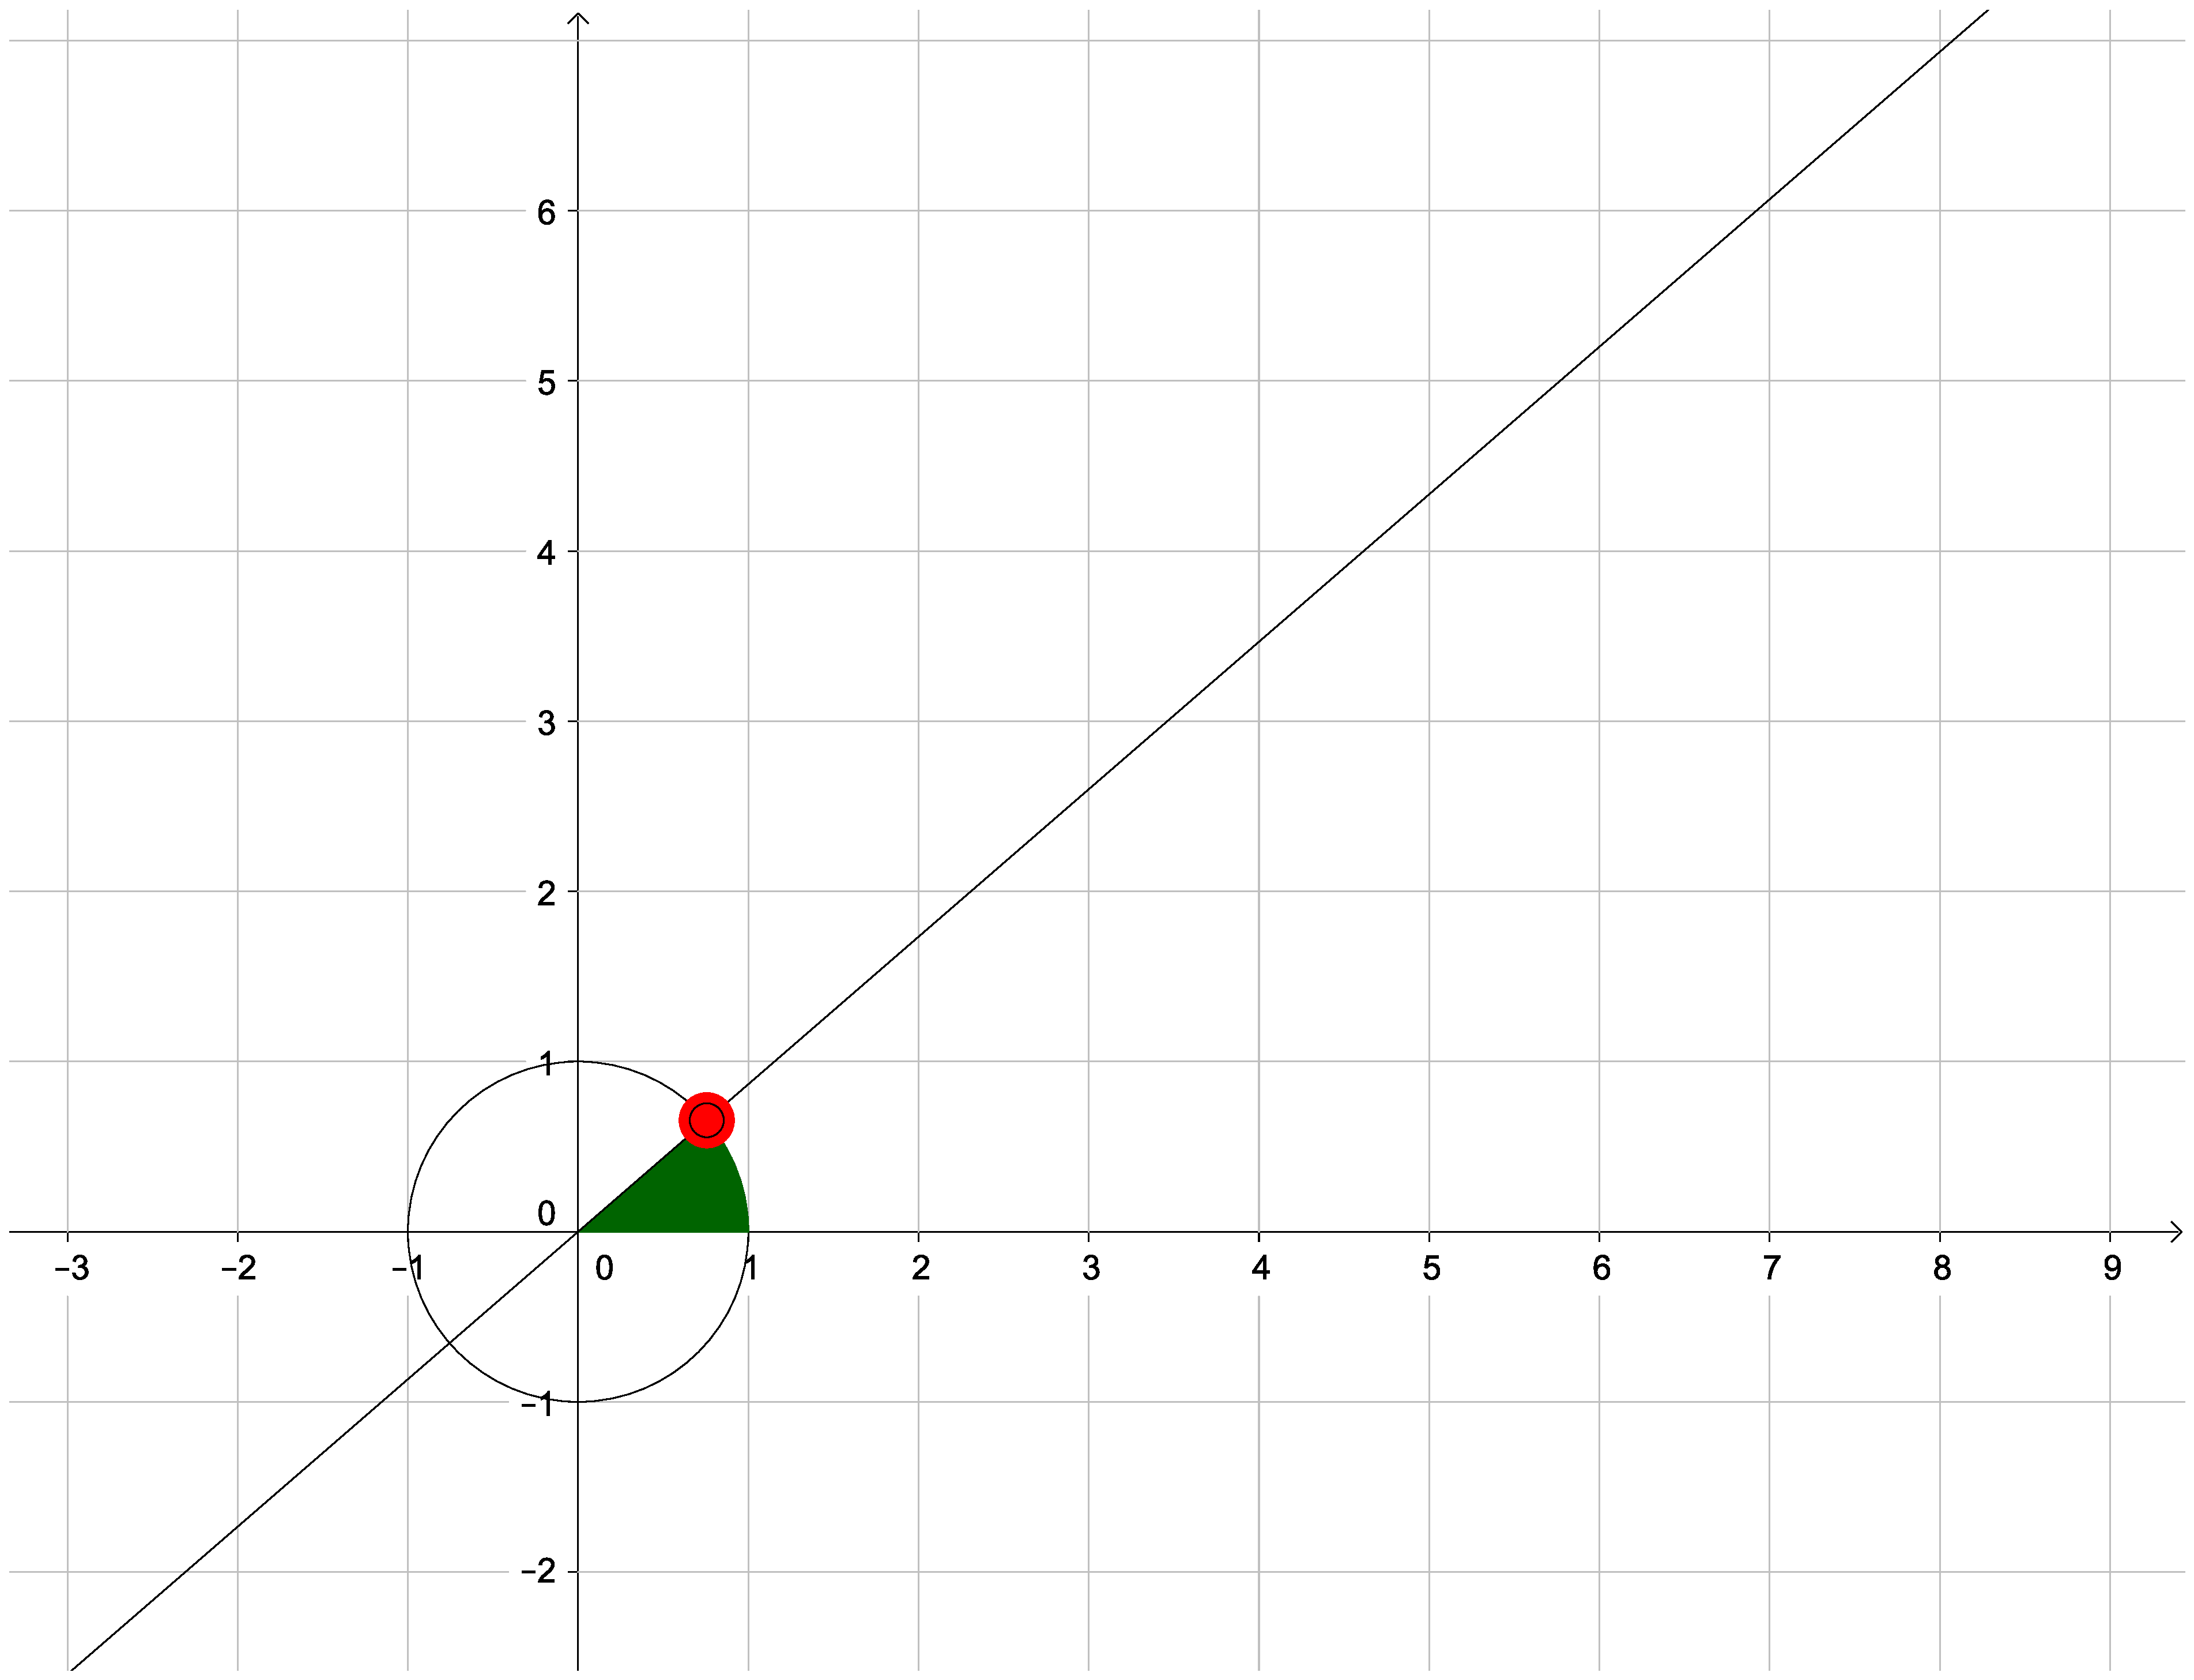
\includegraphics[scale=0.15]{kat.eps}
\end{figure}
\end{przyklad}
\end{frame}

\begin{frame}{Trysekcja kąta}
\begin{przyklad}
Pokażemy, że nie da się podzielić kąta $\frac{2}{3}\pi$ na trzy, czyli skonstruować kąta $\frac{2}{9}\pi$\\
Kąt $\theta$ utożsamiamy z liczbą $e^\theta$.\\
Czyli badamy konstruowalność punku $e^{\frac{2}{9}\pi}=\zeta_9$. Wielomianem minimalnym $\zeta_9$ jest $x^6+x^3+1$, którego stopień to 6. Stąd $\zeta_9$ nie jest konstruowalny.
\end{przyklad}
\end{frame}

\begin{frame}{Podwojenie Objętości sześcianu}
\begin{przyklad}
Problem sprowadza się do skonstruowania liczby $\sqrt[3]{2}$. jego wielomian minimalny to $x^3-2$, jego stopień wynosi $3$. Co oznacza, że $\sqrt[3]{2}$ nie jest konstruowalny.
\end{przyklad}
\end{frame}

\begin{frame}{Teoria Galois}

\end{frame}

\begin{frame}{Liczby konstruowalne}
\begin{twierdzenie}
Niech $\alpha\in\mathbb{C}$ będzie algebraiczne nad $\mathbb{Q}$ i $\mathbb{Q}\subset L$ będzie ciałem rozkładu wielomianu minimalnego $\alpha$ nad $\mathbb{Q}$. Wtedy $\alpha$ jest konstruowalne wtedy i tylko wtedy, gdy $[L:\mathbb{Q}]$ jest potęgą dwójki.
\end{twierdzenie}
\end{frame}


\begin{frame}{Liczby konstruowalne}
\begin{proofs}
$(\Leftarrow)$ Załóżmy, że $[L:\mathbb{Q}]$ jest potęgą dwójki. Ponieważ $L/\mathbb{Q}$ jest Galois, to $|Gal(L/\mathbb{Q})|=[L:\mathbb{Q}]=2^n$. $Gal(L/\mathbb{Q})$ jest rozwiązywalna, więc istnieją podgrupy:
$$\{e\}=G_m\subset G_{m-1}\subset ...\subset G_1\subset G_0=Gal(L/\mathbb{Q})$$ 
takie, że $G_{i-1}$ jest podgrupą normalną dla $G_{i}$ o indeksie 2. Z odpowiedniości Galois wynika, że istnieje wieża ciał
$$\mathbb{Q}=L_{G_0}\subset L_{G_1}\subset...\subset L_{G_m}=L,$$
gdzie $[L_{G_i}:L_{G_{i-1}}]=2$. Zatem $\alpha$ jest konstruowalne.
\end{proofs}
\end{frame}

\begin{frame}{Wielokąty foremne}
\begin{figure}[!htb]
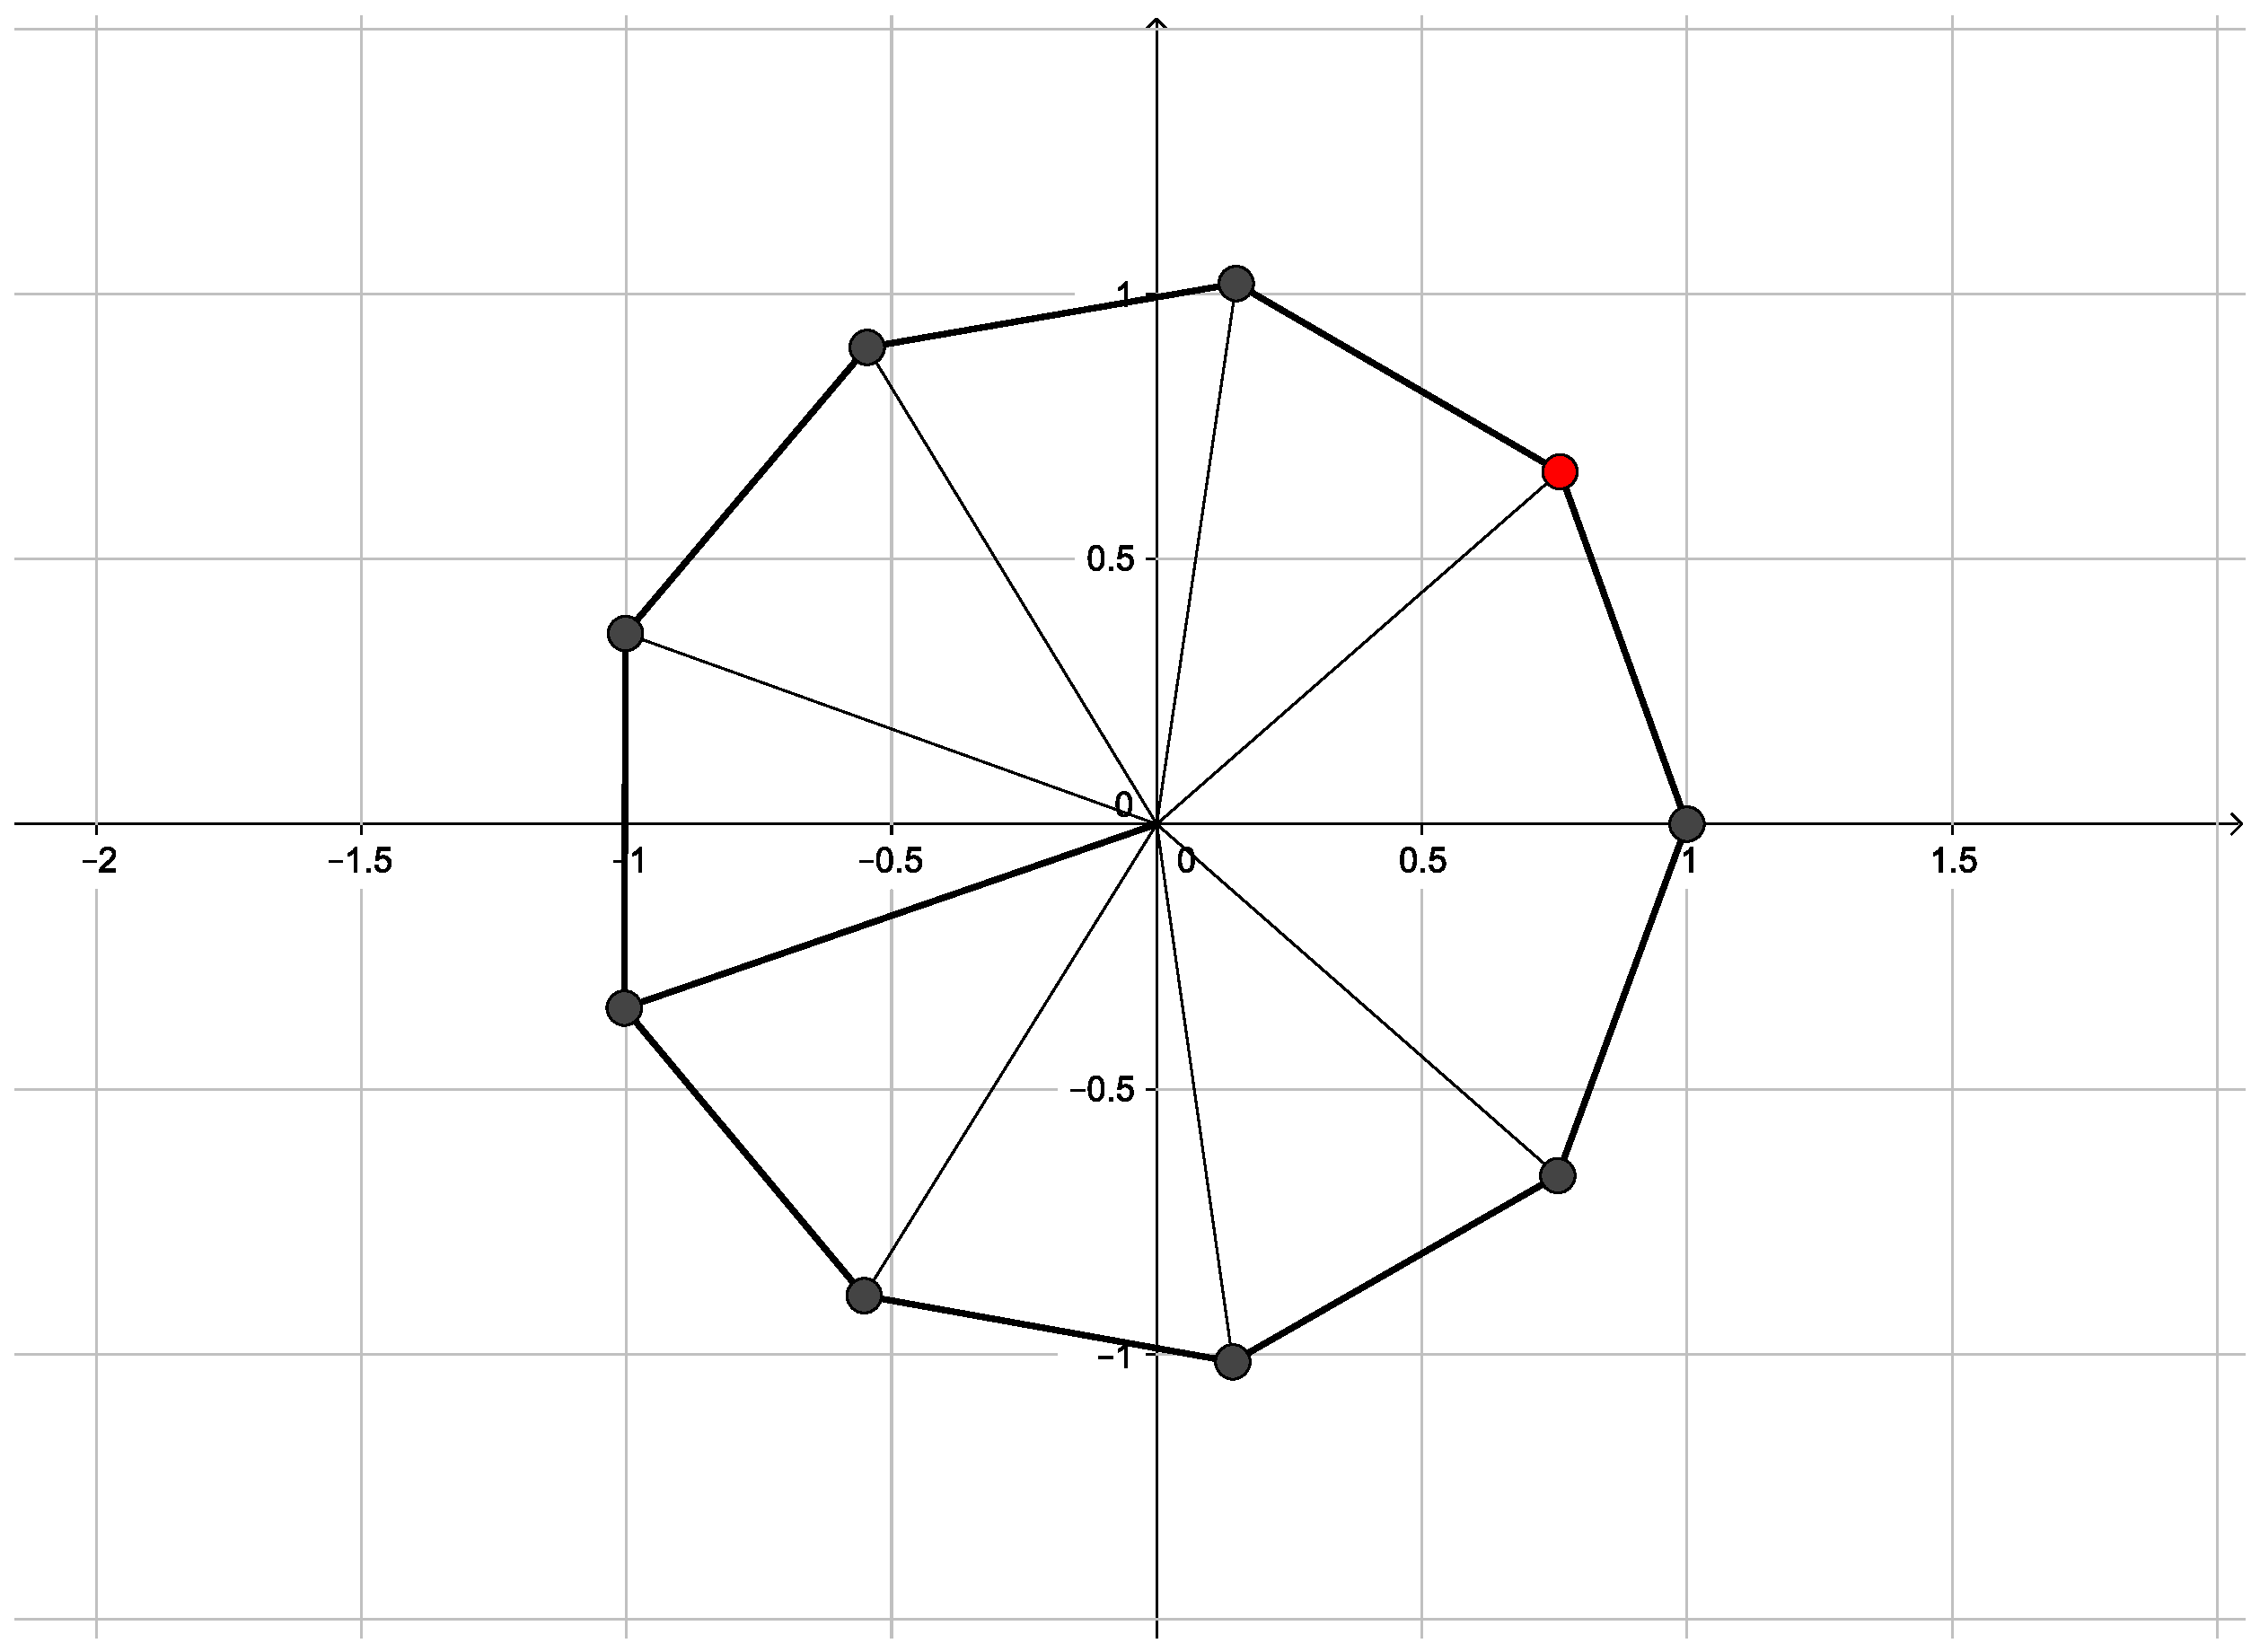
\includegraphics[scale=0.25]{wielokat.eps}
\end{figure}
\end{frame}

\begin{frame}{Wielokąty foremne}
\begin{figure}[!htb]
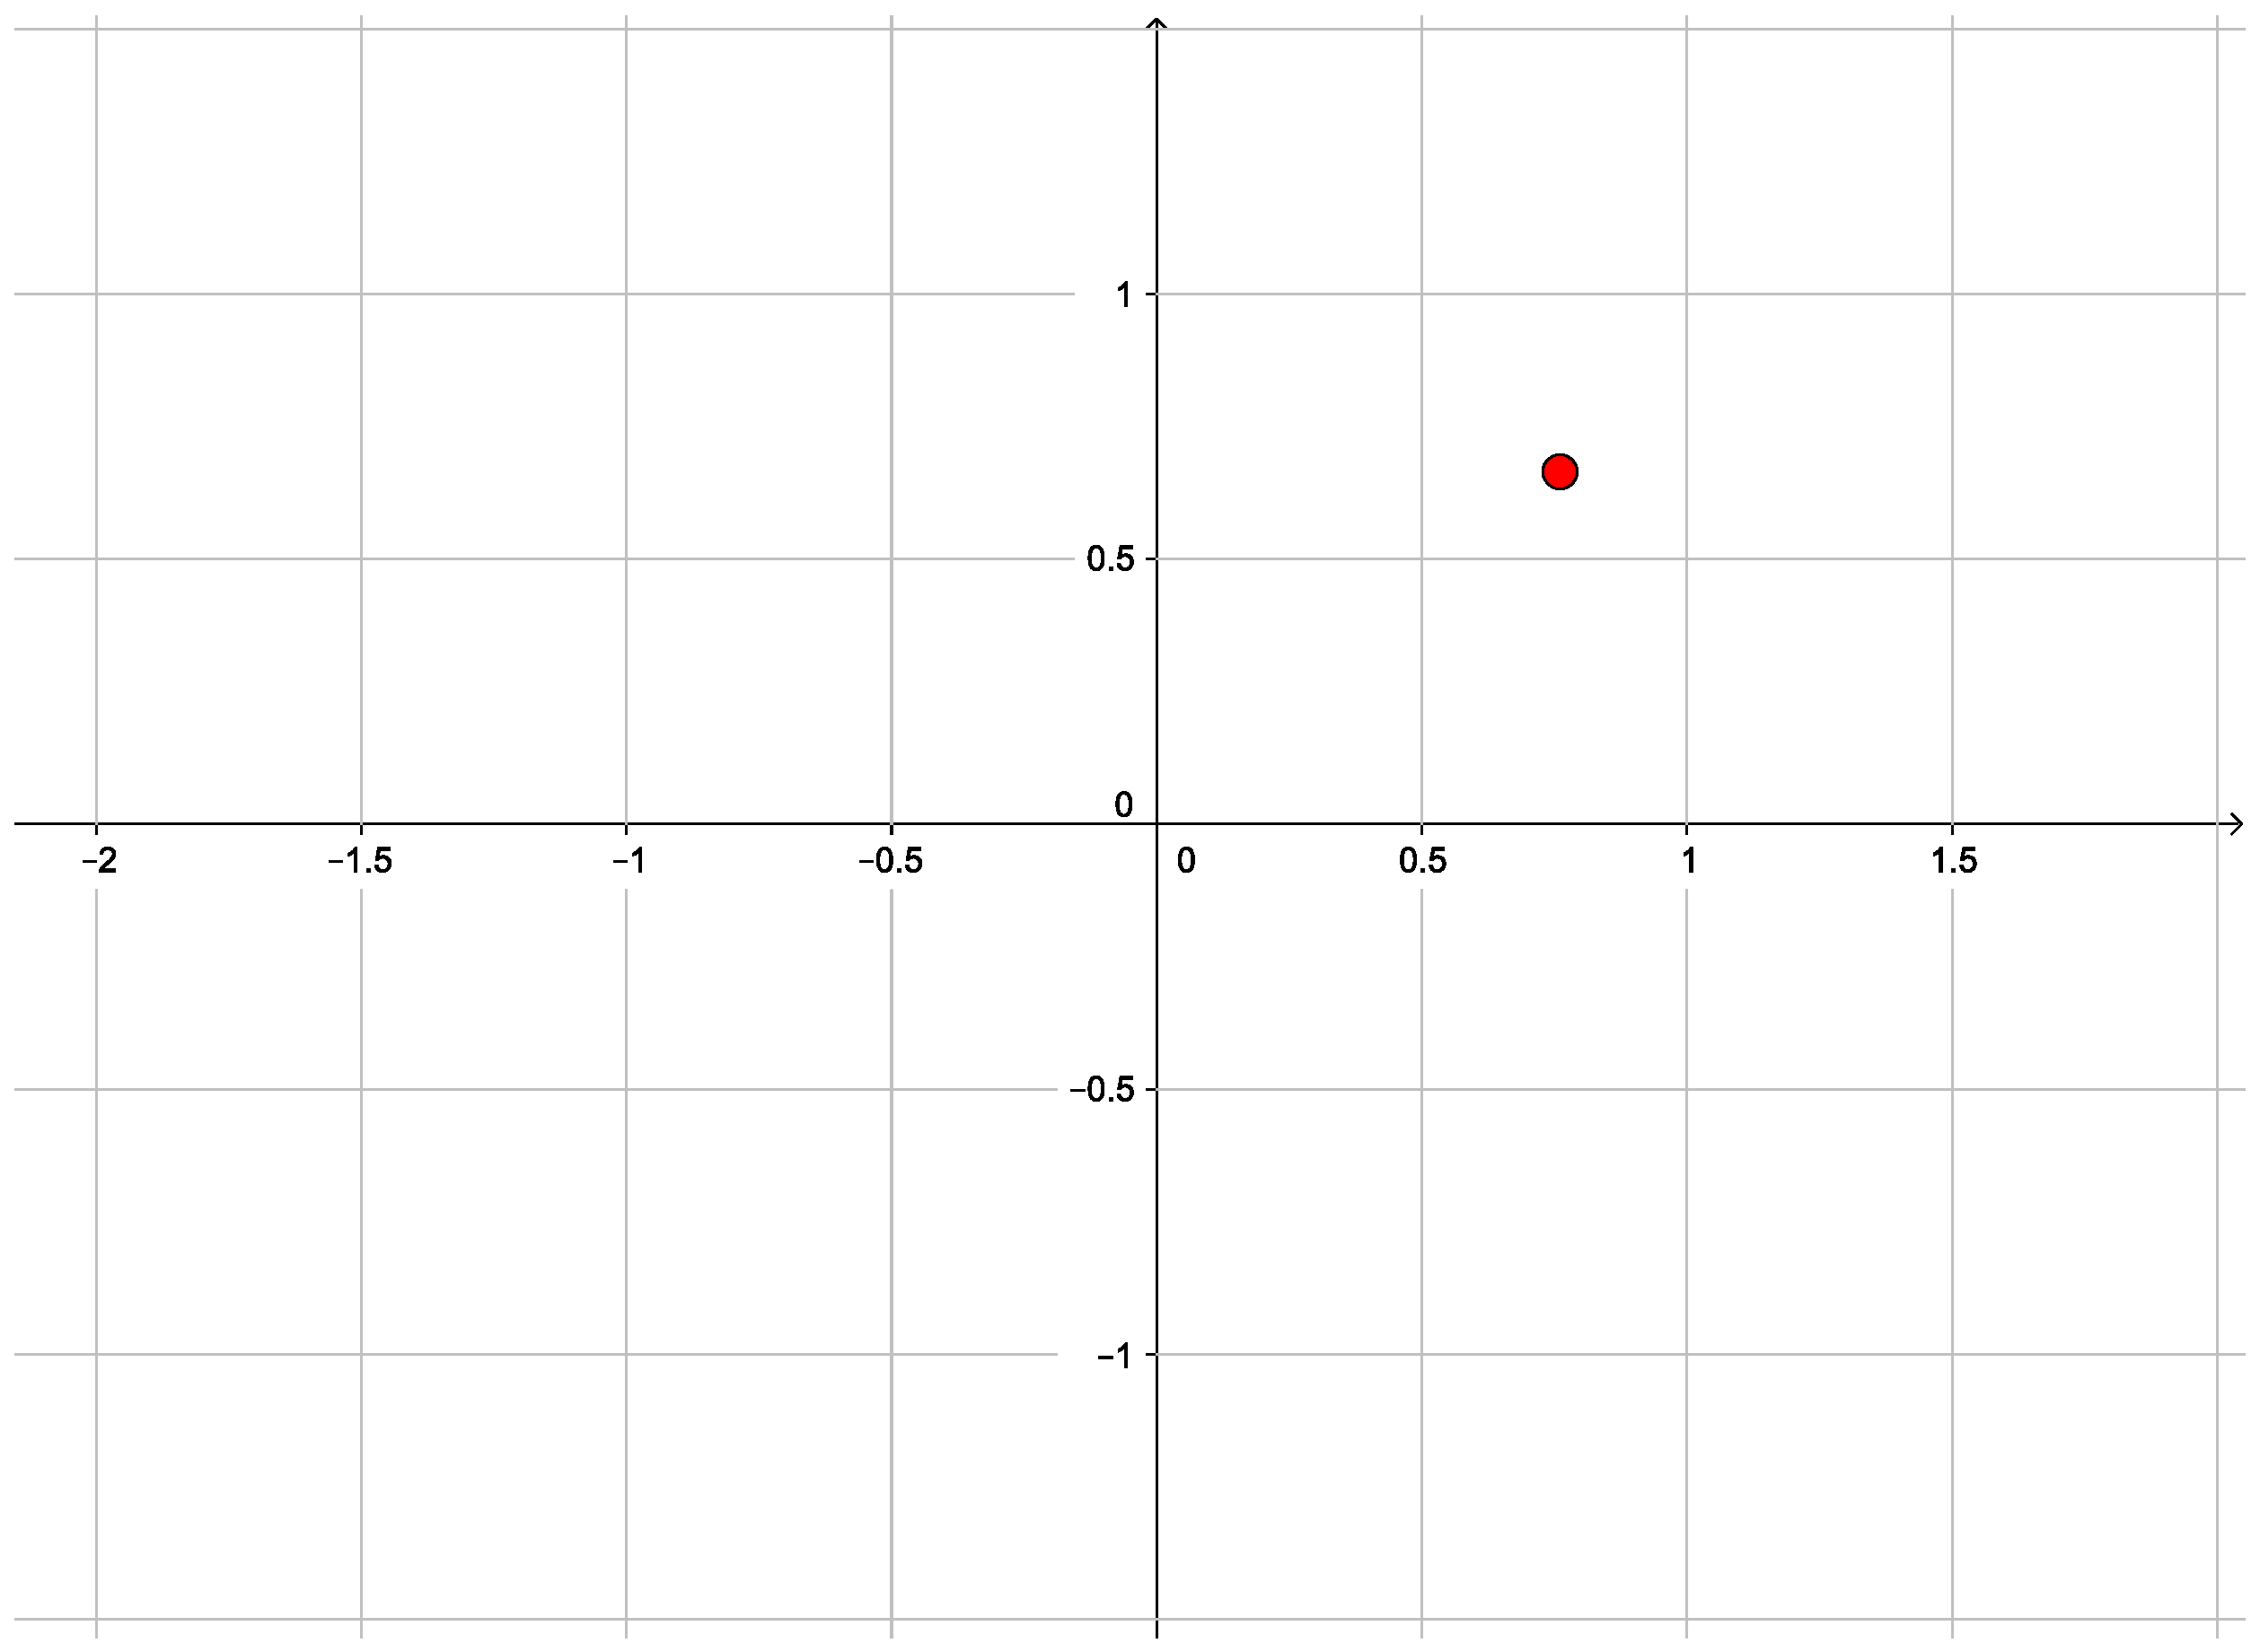
\includegraphics[scale=0.25]{rootu.eps}
\end{figure}
\end{frame}

\begin{frame}{Wielokąty foremne}
\begin{definicja}
Liczba pierwsza $p$ większa od 2 jest liczbą pierwszą Fermata, jeżeli można ją zapisać jako:
$$p=2^{2^n}+1$$
\end{definicja}
\end{frame}

\begin{frame}{Wielokąty foremne}
\begin{twierdzenie}
Niech $n>2$ całkowite, wtedy n-kąt foremny może zostać skonstruowany wtedy i tylko wtedy, gdy
$$n=2^sp_1p_2...p_r,$$
gdzie $p_1,...,p_n$ są liczbami pierwszymi Fermata.
\end{twierdzenie}
\end{frame}

\begin{frame}{Wielokąty foremne}
\begin{proofs}
($\Leftarrow$) Dany n-kąt foremny jest konstruowalny, gdy konstruowalne jest $\zeta_n$.
Wiemy, że:
\begin{itemize}
\item $\mathbb{Q}\subset\mathbb{Q}(\zeta_n)$ jest Galois,
\item $\zeta_n$ jest konstruowalne, gdy $[\mathbb{Q}(\zeta_n):\mathbb{Q}]=2^s$
\item $[\mathbb{Q}(\zeta_n):\mathbb{Q}]=\phi(n)$ 
\end{itemize}
$$\phi(n)=n\prod_{p|n}(1-\frac{1}{p})=\begin{cases}
2^{s-1}(p_1-1)(p_2-1)...(p_n-1)\text{,} & s>0\\
(p_1-1)(p_2-1)...(p_n-1)\text{,} & s=0 \end{cases}$$
w obu przypadkach $[\mathbb{Q}(\zeta_n):\mathbb{Q}]=\phi(n)$ jest potęgą dwójki.
\end{proofs}
\end{frame}

\begin{frame}{Wielokąty foremne}
\begin{proof}
($\Rightarrow$) Niech $n=q_1^{s_1},...,q_n^{s_n}$, gdzie $q_1,...,q_n$ są liczbami pierwszymi.
$$\phi(n)=n\prod_{q|n}(1-\frac{1}{q})=q_1^{a_1}(q_1-1)...q_2^{a_2}\textsl{•}(q_2-2).$$
Jeżeli $q_i$ jest większe od 2, to $s_i$ jest równe 1, dla 2 dowolne. Zatem wszystkie liczby   $q_1,...,q_n$ są postaci $2^{k_i}+1$. Wystarczy dowieść, że jeżeli liczba pierwsza tej postaci jest liczbą Fermata.
\end{proof}
\end{frame}

\begin{frame}{Liczby Origami}
\begin{figure}[!htb]
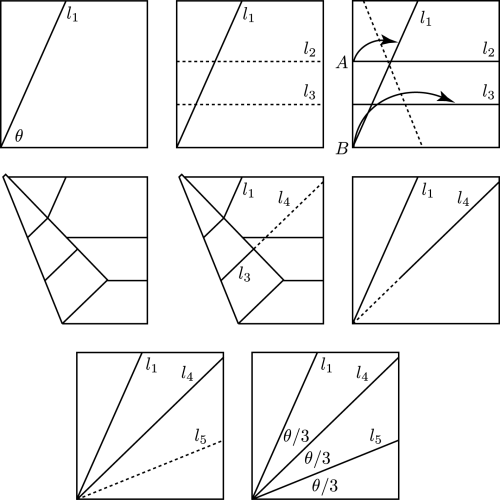
\includegraphics[scale=2]{origamitrisection.png}
\end{figure}
\end{frame}

\begin{frame}{Liczby Origami}
\begin{figure}[!htb]
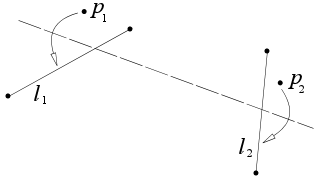
\includegraphics[scale=2]{Huzita_axiom_6.png}
\end{figure}
\end{frame}

\begin{frame}{Liczby Origami}
\begin{lemat}
Niech $P_1$ będzie punktem na płaszczyźnie nie leżącym na linii $l_1$. Linia $l$, o którą odbicie $P_1$ leży na prostej $l_1$, jest styczna z parabolą o ogniskowej w $P_1$ i kierownicy $l_1$.
\end{lemat}
\end{frame}

\begin{frame}{Liczby Origami}
\begin{przyklad}
pokażemy, jak za pomocą stycznej do 2 paraboli policzyć pierwiastki wielomianu $x^3+ax+b=c$
rozważmy parabole
$$(y-\frac{a}{2})^2=2bx \text{ oraz } y=\frac{1}{2}x^2$$
Niech $l$ będzie prostą styczną do tych parabol. w punktach $(x_1,y_1)$ pierwszą oraz $(x_2,y_2)$ drugą. współczynnik nachylenia prostej wynosi:
$$m=\frac{b}{y_1-\frac{1}{2}a}$$
stąd $m\not=0$ oraz:
$$x_1=\frac{zb}{2m^2}$$
$$y_1=\frac{zb}{m}+\frac{a}{2}$$
\end{przyklad}
\end{frame}

\begin{frame}{Liczby Origami}
\begin{przyklad}
Jeśli podstawimy pod $m=\frac{y_1-y_2}{x_1-x_2}$ otrzymamy:
$$m=\frac{y_1-y_2}{x_1-x_2}=\frac{\frac{m^2}{2}-(\frac{b}{m}+\frac{a}{2})}{m-\frac{2}{2m^2}}=\frac{m^4-2m-qm^2}{2m^3-b}$$
Co sprowadza się do:
$$m^3+am^2+bm+c=0$$
\end{przyklad}
\end{frame}

\begin{frame}{Liczby Origami}
\begin{figure}[!htb]
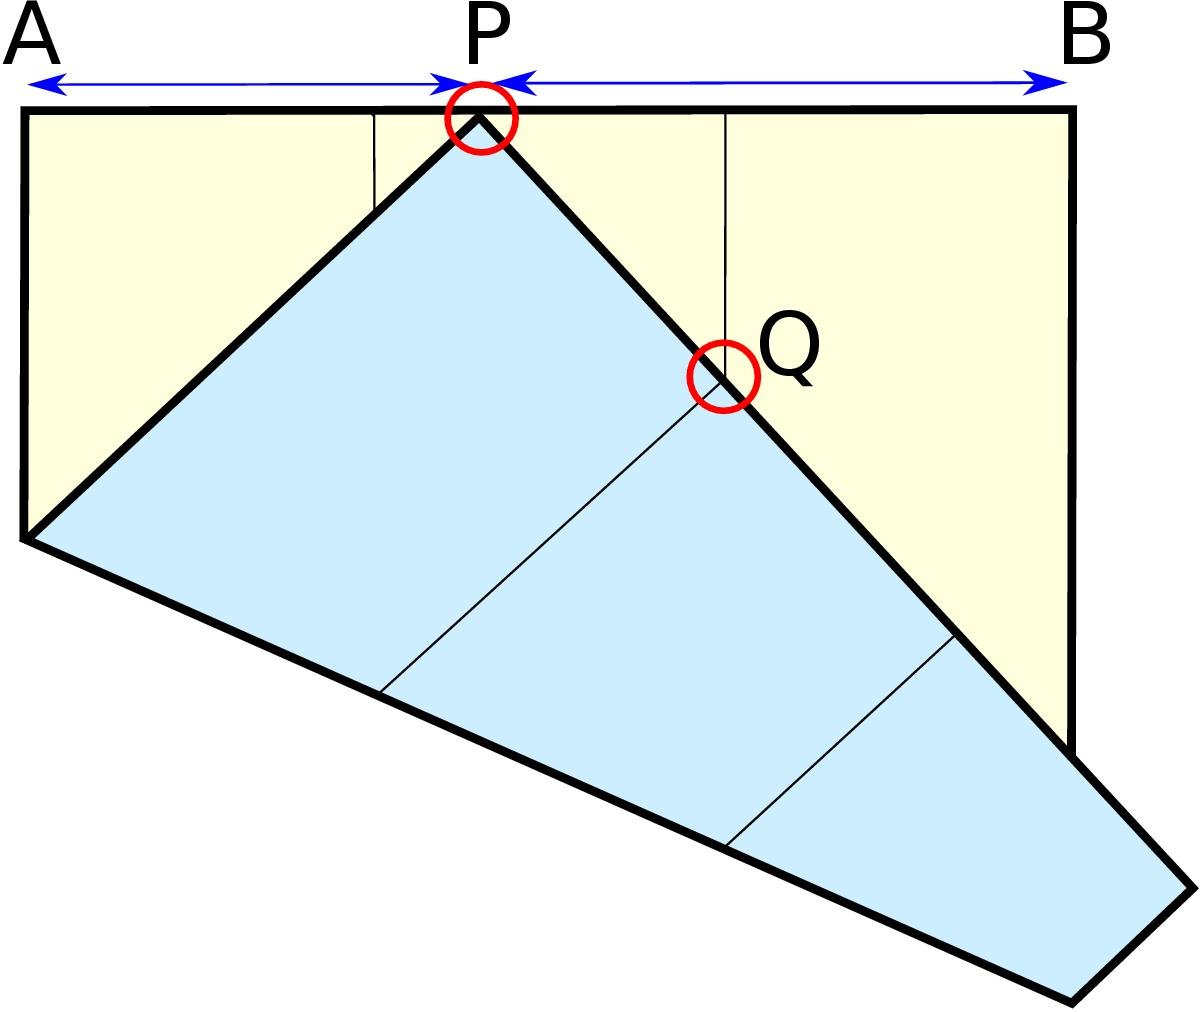
\includegraphics[scale=0.2]{root.jpg}
\end{figure}
\end{frame}

\begin{frame}{Liczby Origami}
\begin{twierdzenie}
Niech $\mathcal{O}=\{\alpha\in\mathbb{C}\ |\ \alpha\ jest\ origami\}$. $\mathcal{C}$ jest podciałem 	$\mathbb{C}$ Ponadto: 
\begin{enumerate}[label=(\alph*)]
\item Niech $\alpha = a + bi\in\mathcal{C}$, gdzie $a,b\in\mathbb{R}$, to $a,b\in\mathcal{C}$.
\item Jeżeli $\alpha \in \mathcal{C}$, to $\sqrt{\alpha}\in\mathcal{C}$
\item Jeżeli $\alpha \in \mathcal{C}$, to $\sqrt[3]{\alpha}\in\mathcal{C}$
\end{enumerate}
\end{twierdzenie}
\end{frame}

\end{document}
